% Appendix A


%----------------------------------------------------------------------------------------
%----------------------------------------------------------------------------------------
%----------------------------------------------------------------------------------------
\chapter{Detailed high-level description of the components of \textit{RootSkel}}

\newpage
\begin{table}[H]
	\centering
	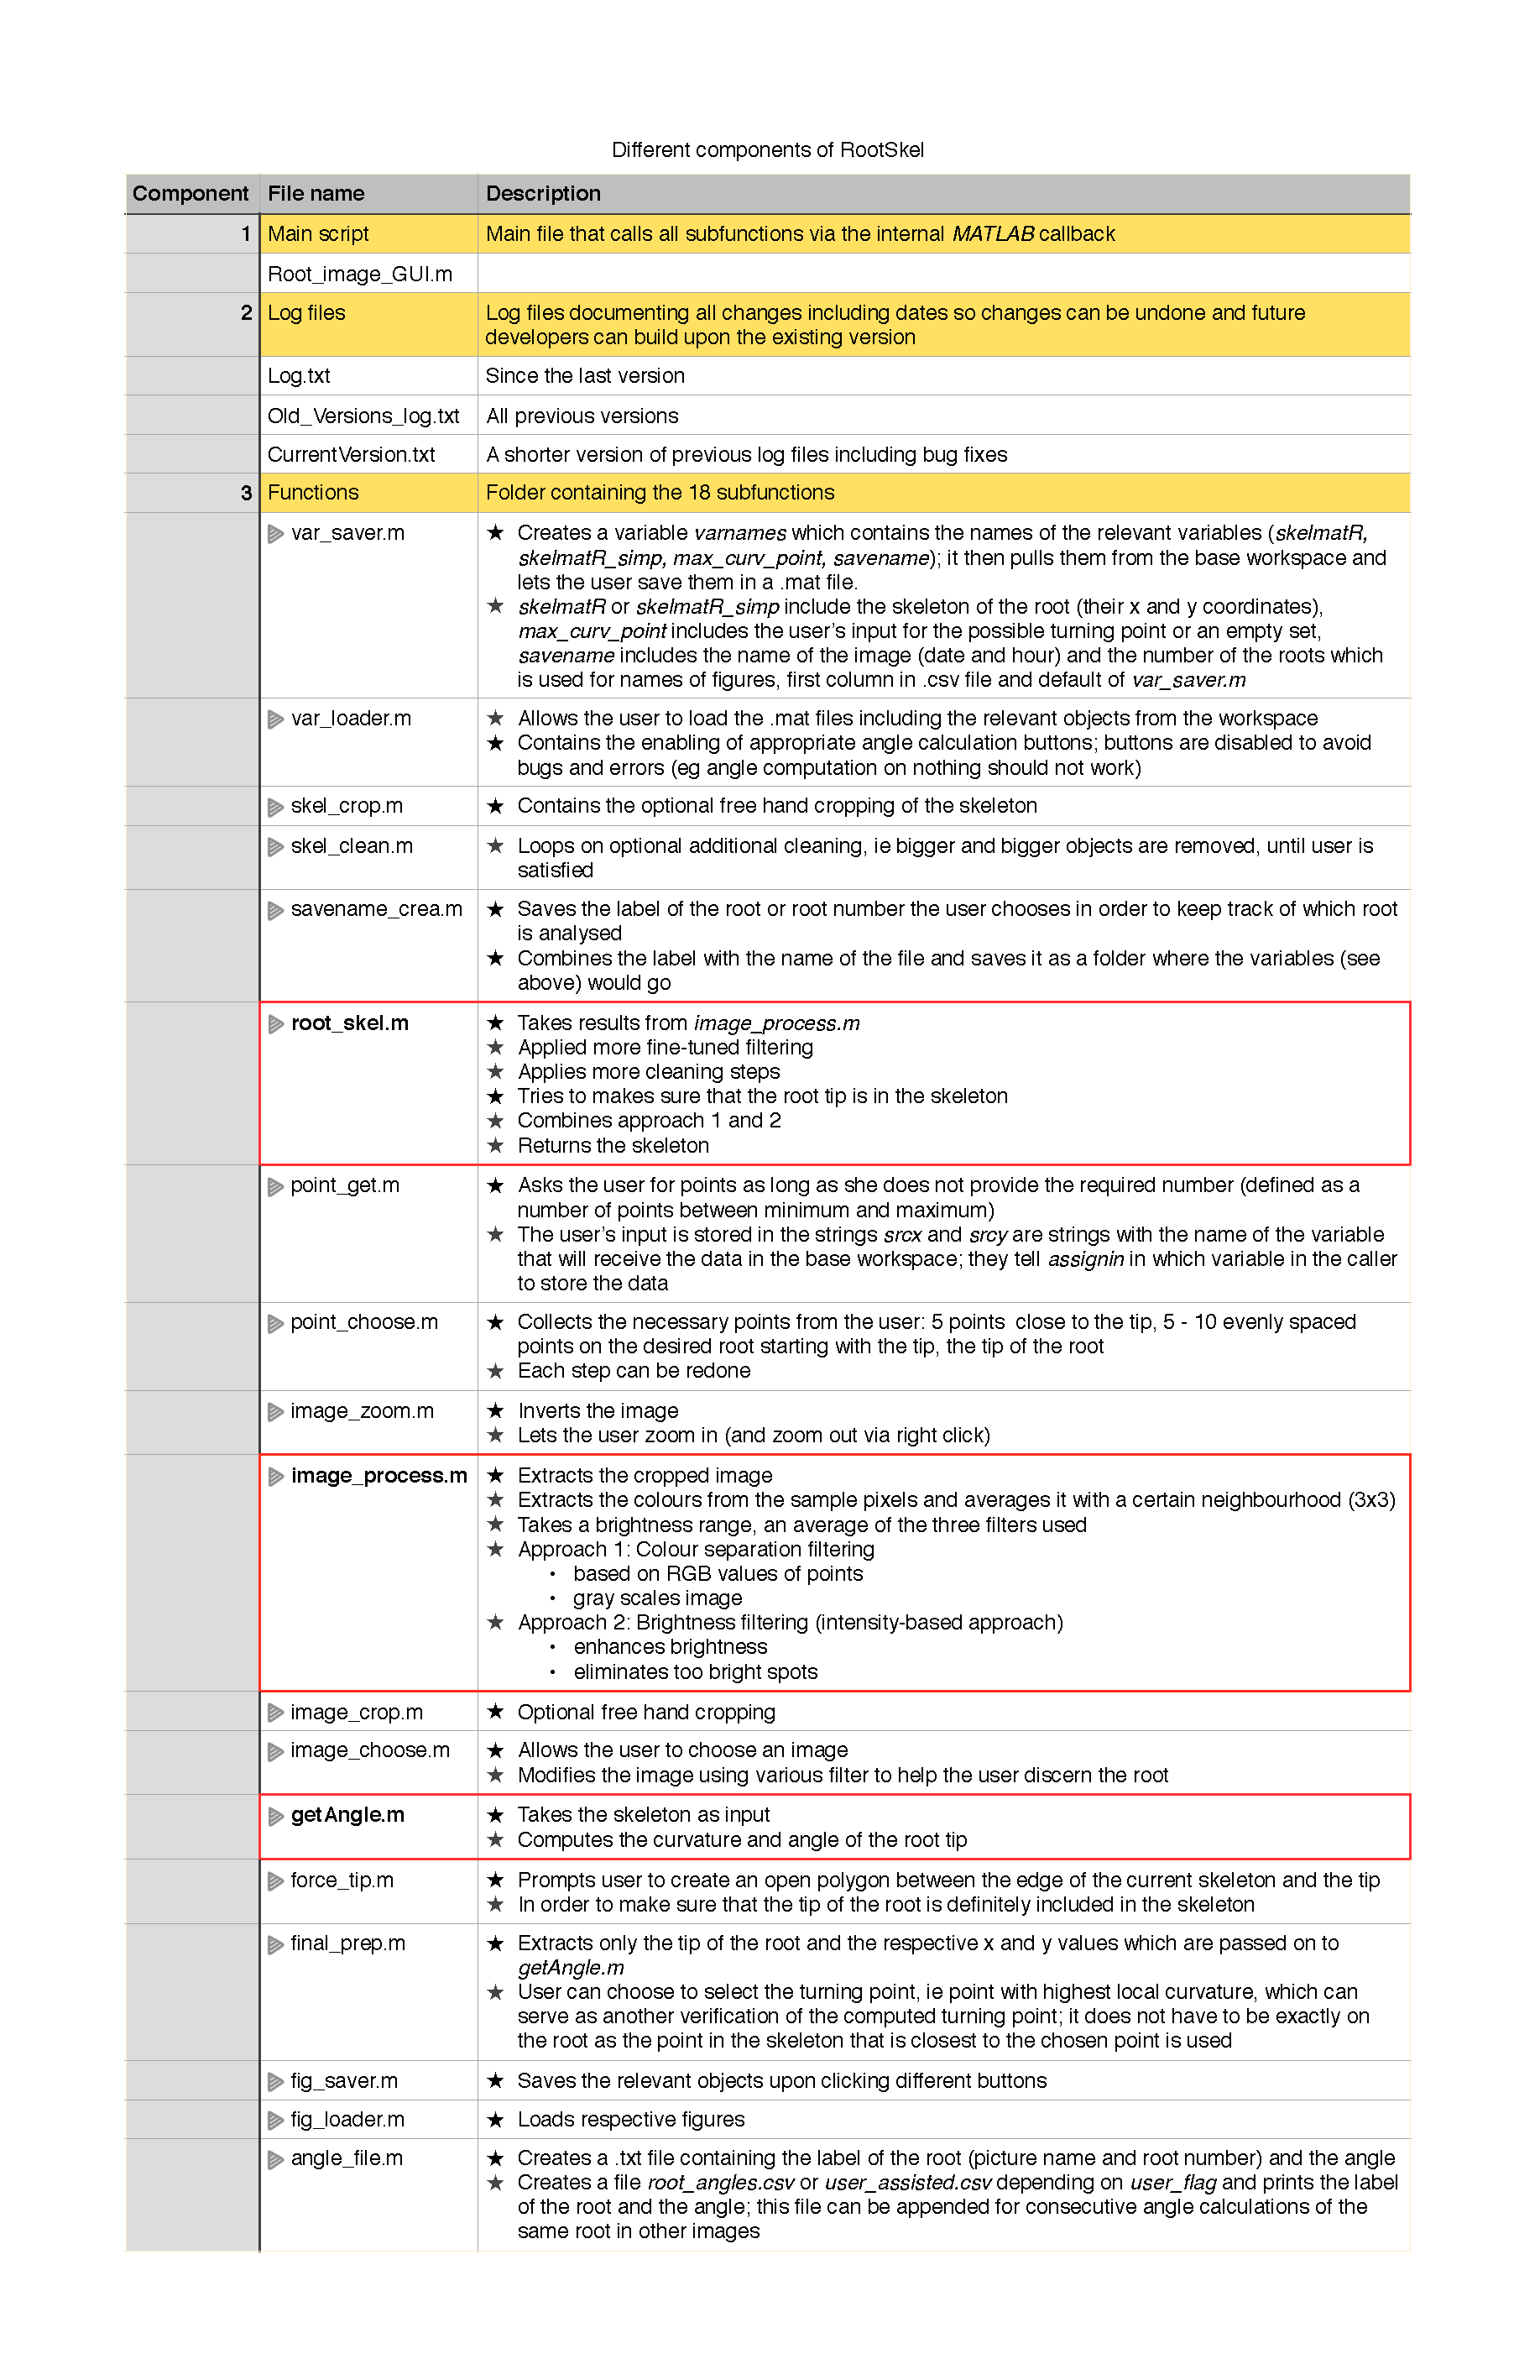
\includegraphics[width=1.\textwidth]{../Figures/components2.pdf}
	\caption{The different components and modules of \textit{RootSkel} with a description of each of them; the most important ones containing the core functionality of \textit{RootSkel} are framed in red, the high-level components are shaded in yellow. A version of increased font size can be found on \url{https://github.com/burfel/root-tip-angle/blob/master/report/Figures/components.pdf}.}
	\label{table:modules}
\end{table}



%----------------------------------------------------------------------------------------
%----------------------------------------------------------------------------------------
%----------------------------------------------------------------------------------------
\chapter{Manual for \textit{RootSkel}}\label{chp:manual}


%----------------------------------------------------------------------------------------
%----------------------------------------------------------------------------------------
\section{Key features} %SHOW HOW ELEABORATE TOOL IS

Figure \ref{fig:workflow} explains the key components of %this image-analysis software tool 
\textit{RootSkel} to address the problem of highly noisy electrotropism consumer camera images of Arabidopsis roots and a standardised way of computing the angle for the curved root tip. 
The tool takes the form of a MATLAB program and subprograms with a GUI on top of it.

%----------------------------------------------------------------------------------------
\subsection{Handling user's mistakes}

When we take the user's input, e.g. choosing samples along the root, we correct for small mistakes by taking a neighbourhood (3\(\times\)3) average around the pixel. 
%followed by adaptive thresholding.
This means the user does not have to take special care when choosing the points as long as it is in the approximate region of the root.

%----------------------------------------------------------------------------------------
\subsection{User interaction and optional steps}
The software tool was created in ways that it is easy to interact with for a future user. 
We implemented several optional steps that only need to be performed if the user thinks they are necessary. This on the one hand saves time in the preprocessing but on the other hand also ensures that tricky roots can be tackled by various optional steps in order to extract a skeleton. 

%----------------------------------------------------------------------------------------
\subsection{Drawing the angle}
The GUI lets the user visualise the angle that is computed. This not only helps to make the tool more visual and transparent, but can also assist in debugging. 



%%----------------------------------------------------------------------------------------
%%----------------------------------------------------------------------------------------
%%----------------------------------------------------------------------------------------
%\chapter{Other programming languages}
%
%Even though MATLAB has several advantages, it might be worth looking into alternative non-proprietary programming languages to make the tool accessible to a wider public or other options of making the tool portable, i.e. without requiring the user to have MATLAB installed.
%Alternative languages one might want to consider are \textit{Python} and \textit{Julia}. Another recommended language is \textit{OpenCV} as it is very fast and well documented. Other non-open source software such as \textit{ImageJ}, a Java based image processing program, and \textit{Avizo} which is a general-purpose commercial software application for scientific and industrial data visualisation and analysis with a nice GUI, were not investigated further in this work. 


%----------------------------------------------------------------------------------------
%----------------------------------------------------------------------------------------
\section{\textit{RootGUI} for Dummies}

%REMARK: \textit{For environmental reasons, we do not show \textit{RootGUI}, the manual of \textit{RootSkel} in the printed version. We refer to the electronic version on \url{https://github.com/burfel/root-tip-angle/blob/master/report/main.pdf} to view the easy to read and fun \textit{RootGUI} for Dummies manual. To leave the rest identical to the electronic version, we keep the page numbers from the full (electronic) version of the report.}

%----------------------------------------------------------------------------------------
\subsection{Intro}

Hello and welcome! 
So this is is your first time operating \textit{RootGUI}, the GUI of \textit{RootSkel}. Excited?
For the next 5 minutes or so I'll be your friendly instruction manual on how to use \textit{RootGUI}. 
You have downloaded the current version of \textit{RootSkel} from \url{https://github.com/GiovanniSena/Auto-angle} and you have MATLAB installed on your computer? Then let's get right down to business.

First of all, open your \textit{MATLAB}. You should view something similar to this::
\begin{figure}[H]
	\centering
	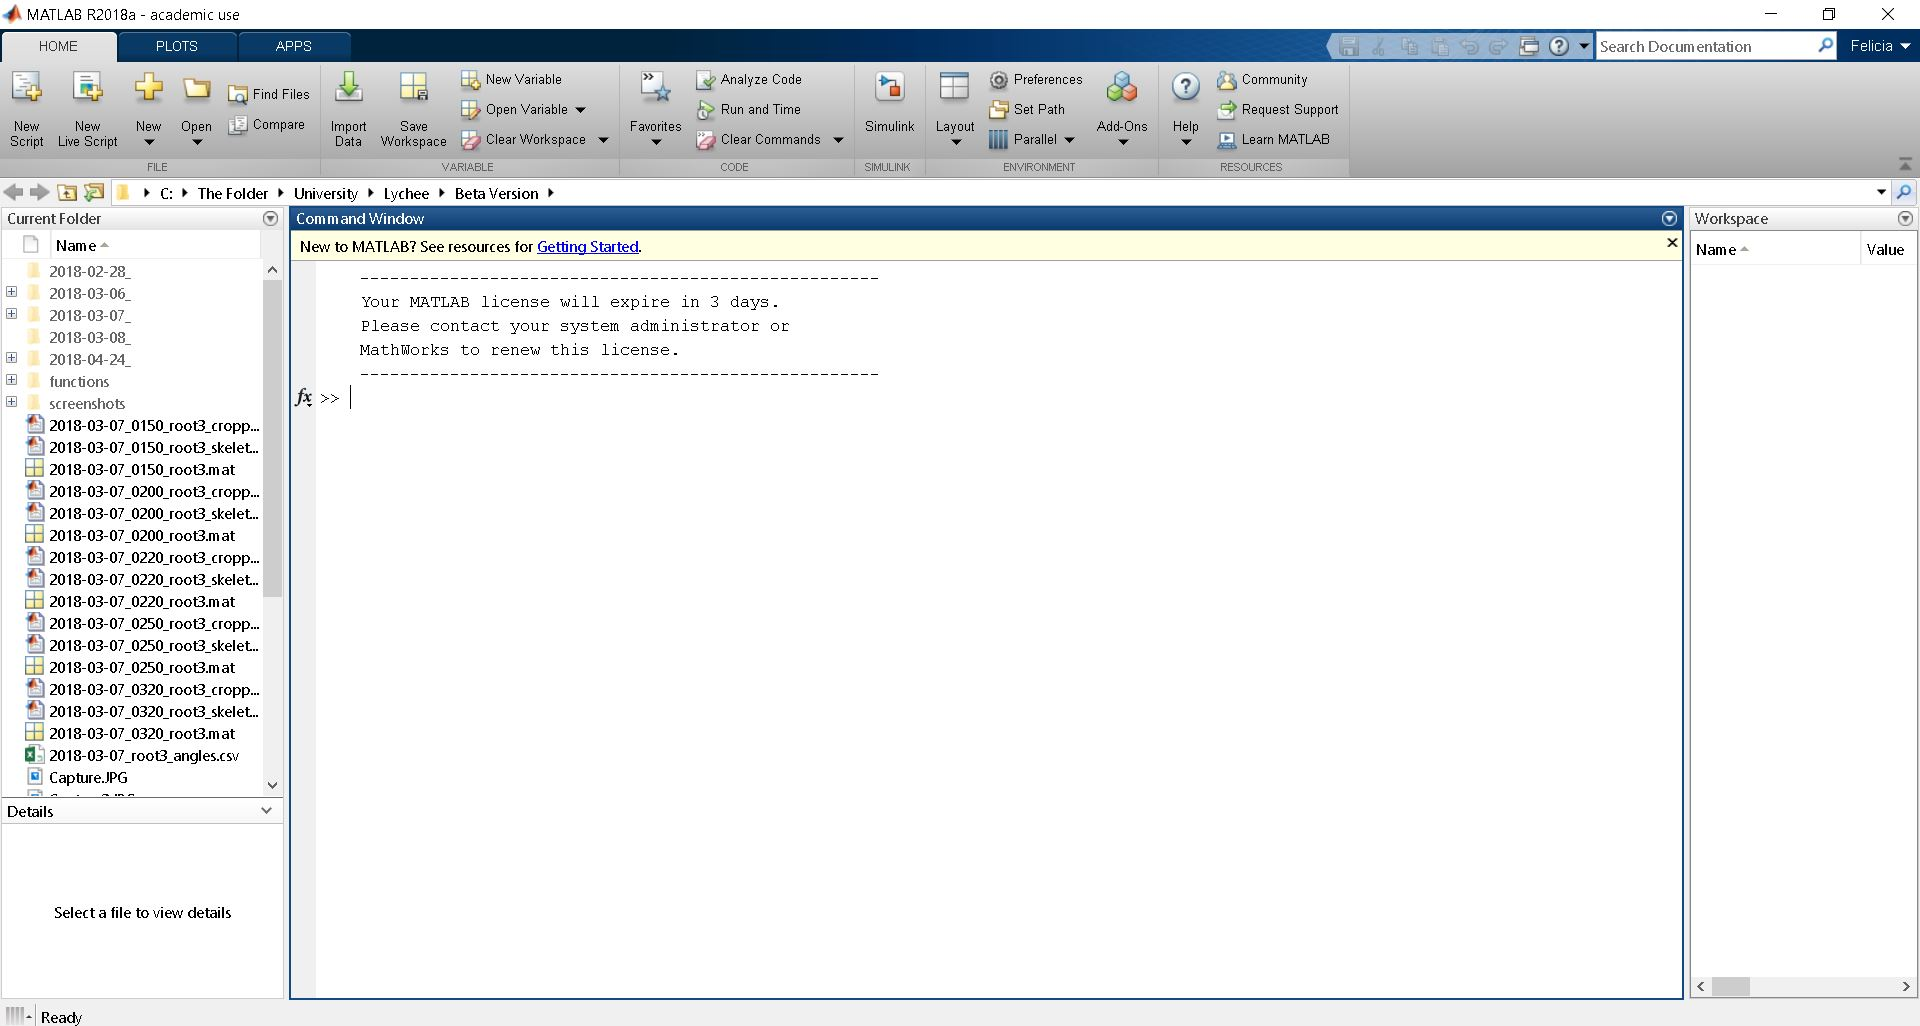
\includegraphics[width=\textwidth]{../Figures/manual/intro1.jpg}
	\caption{The MATLAB GUI}
	\label{fig:img1}
\end{figure}

And now, in order to bring \textit{RootGUI} up, navigate to the folder where \textit{RootSkel} is located on the LHS, and type \textit{Root\_image\_GUI} in the MATLAB console as shown in figure \ref{fig:img2}.
\begin{figure}[H]
	\centering
	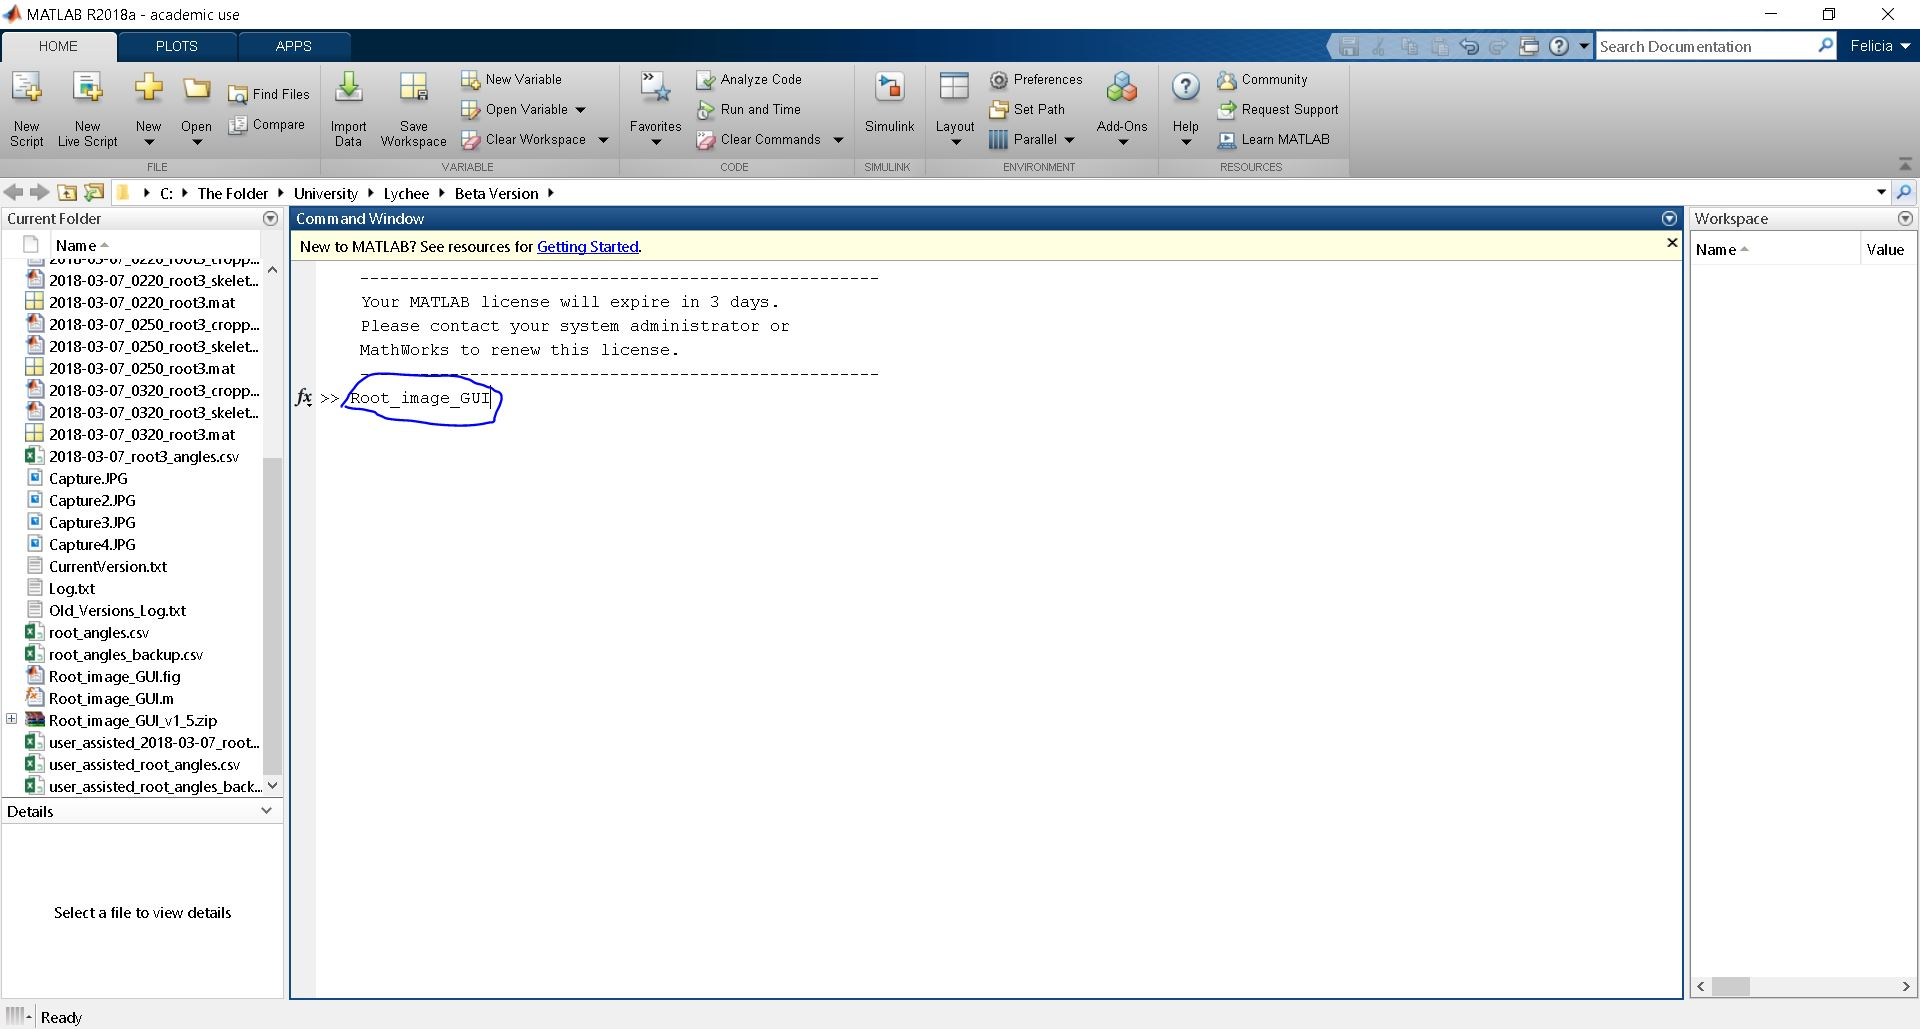
\includegraphics[width=\textwidth]{../Figures/manual/intro2.jpg}
	\caption{Calling \textit{Root\_image\_GUI} from the MATLAB console}
	\label{fig:img2}
\end{figure}

Then press enter and voil\`a!
\begin{figure}[H]
	\centering
	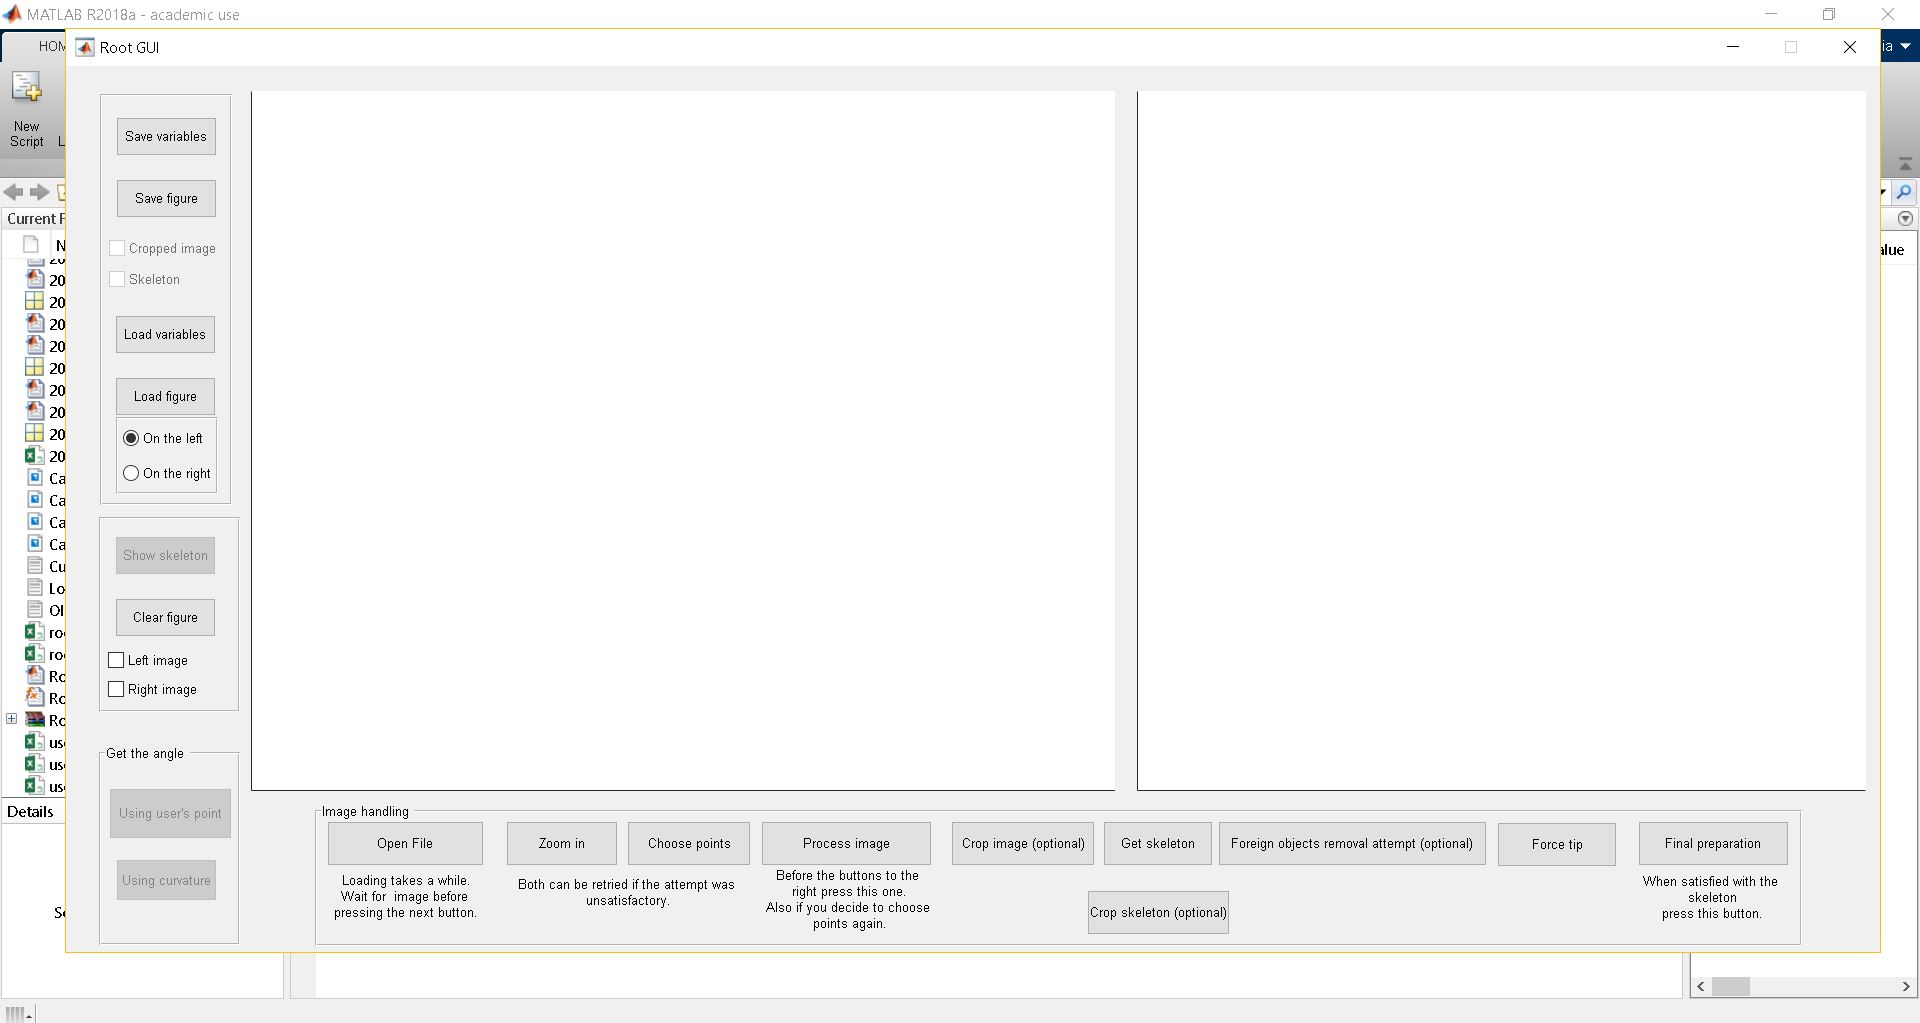
\includegraphics[width=\textwidth]{../Figures/manual/intro3.jpg}
	\caption{The \textit{RootGUI}}
	\label{fig:img3}
\end{figure}

There you go, you have opened the GUI! You've successfully completed the first step.

%----------------------------------------------------------------------------------------
Now let's get ourselves some angles.
\subsection{Getting the angles -- main route}

First, we want to open an image with the roots.
 \begin{figure}[H]
 	\centering
 	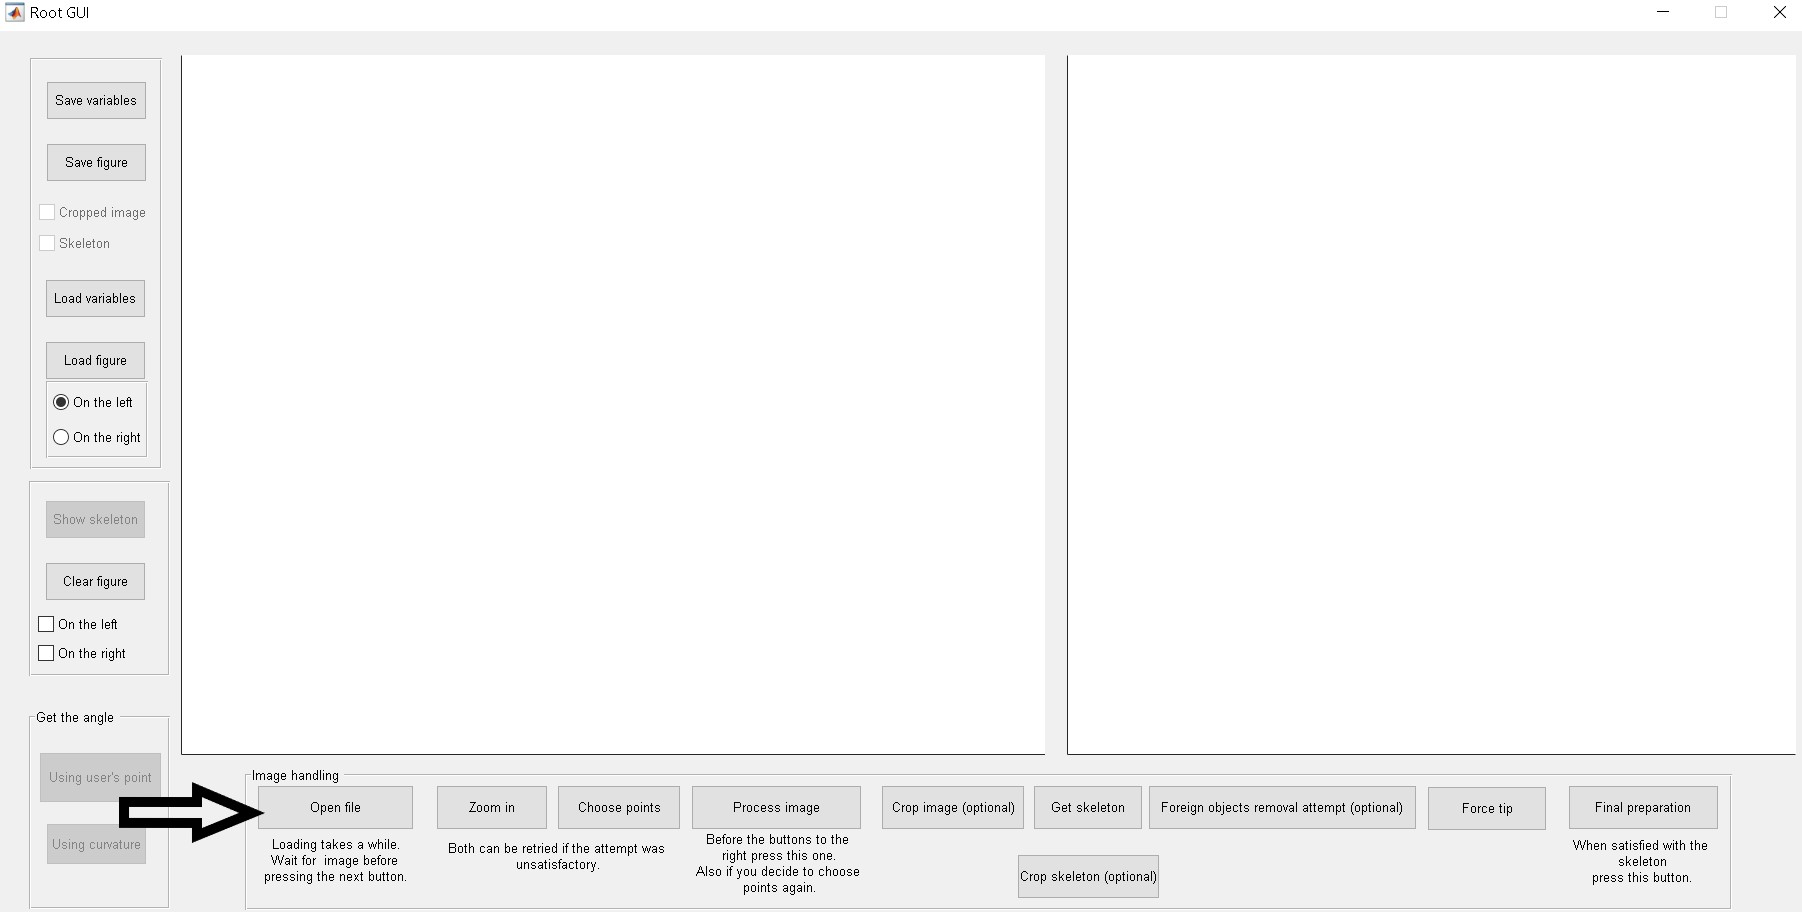
\includegraphics[width=\textwidth]{../Figures/manual/step1.jpg}
 	\caption{Step 1 in the \textit{RootSkel} pipeline: Opening a file}
 	\label{fig:img4}
 \end{figure}
 
 We click the \textit{Open file} button and you are prompted to choose an image.
 \begin{figure}[H]
 	\centering
 	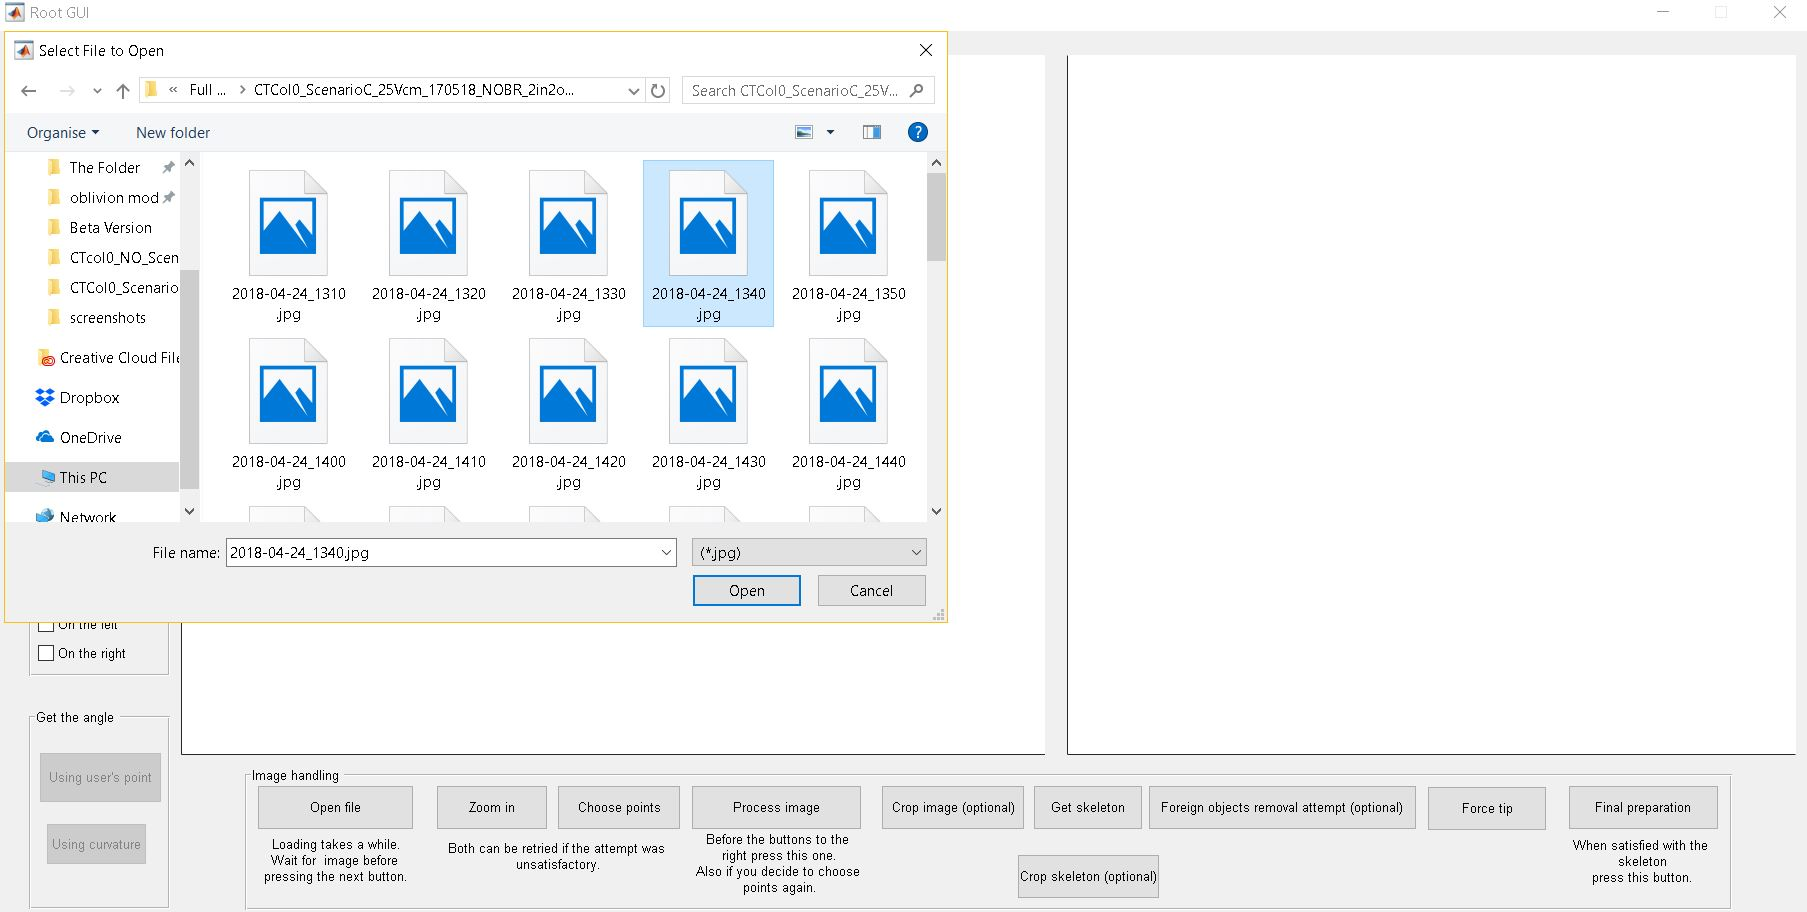
\includegraphics[width=\textwidth]{../Figures/manual/step2.jpg}
 	\caption{Choosing a file}
 	\label{fig:img5}
 \end{figure}
 
 Now that we chose our image, the next thing we should do is to zoom in on the root we want to work on. 
 For that, we click on the \textit{Zoom in} button.
 \begin{figure}[H]
 	\centering
 	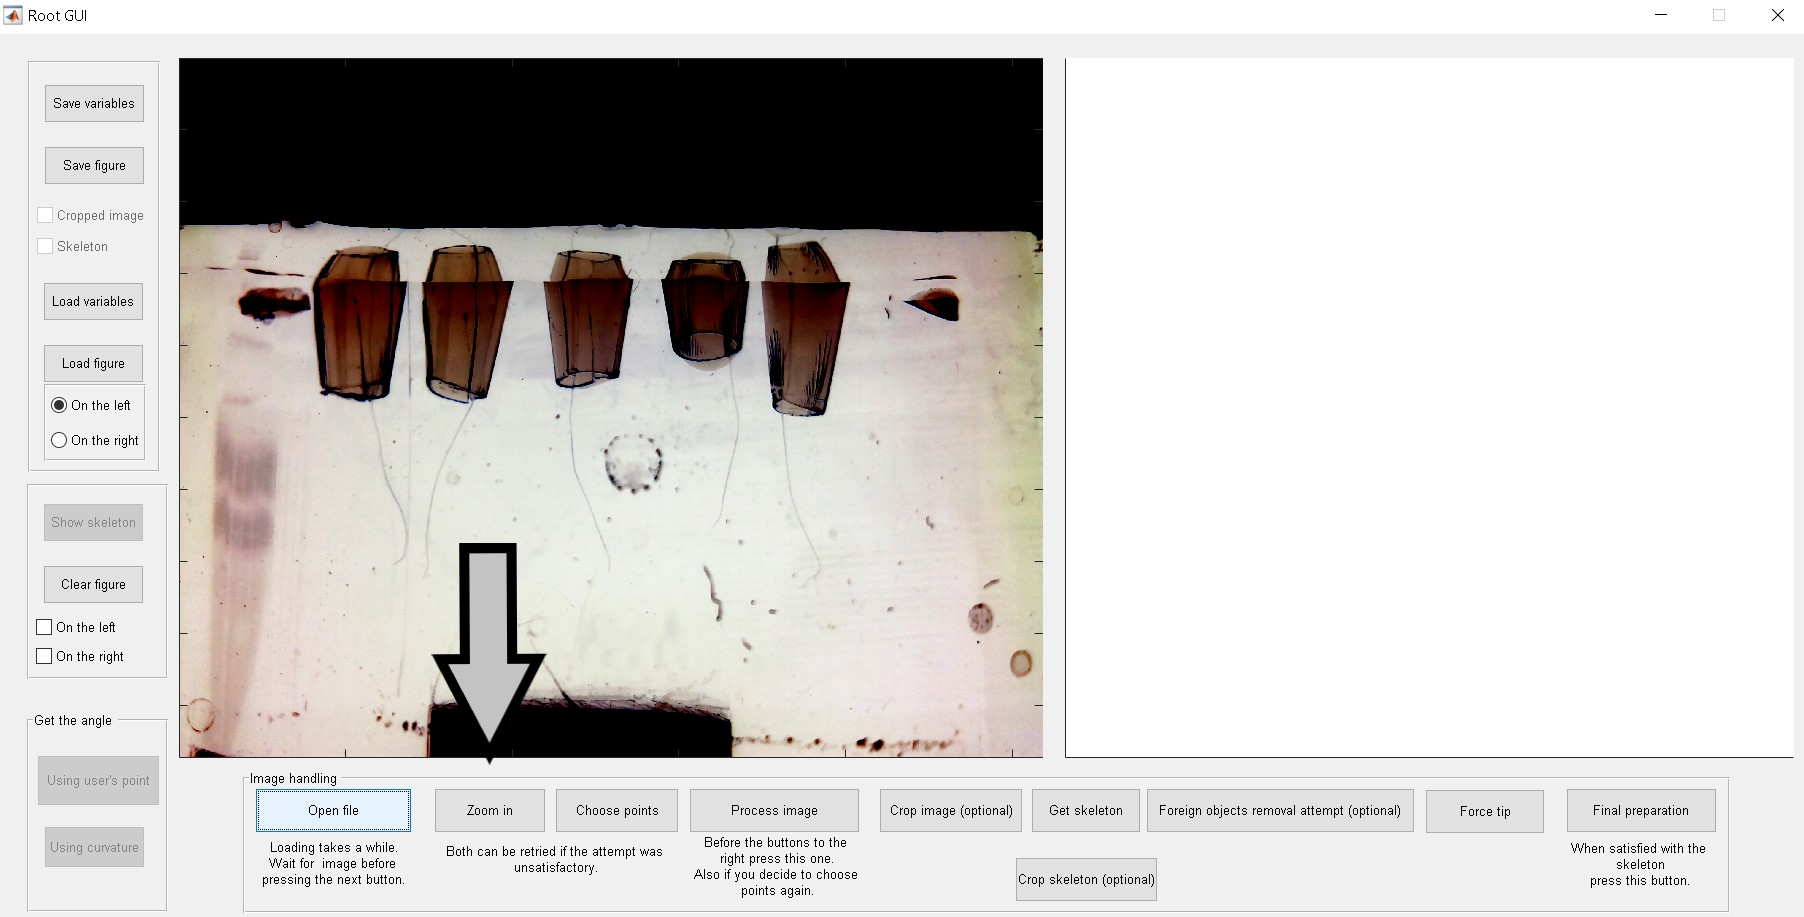
\includegraphics[width=\textwidth]{../Figures/manual/step3.jpg}
 	\caption{Step 2 in the \textit{RootSkel} pipeline: Zooming in on the desired root}
 	\label{fig:img6}
 \end{figure}
 
 After you clicked the button, you will be prompted to zoom in on the desired root (see figure \ref{fig:img7})
 and you will go on to drag a rectangle around the desired root (see figure \ref{fig:img8}).
 	
\begin{figure}[H]
 	\centering
 	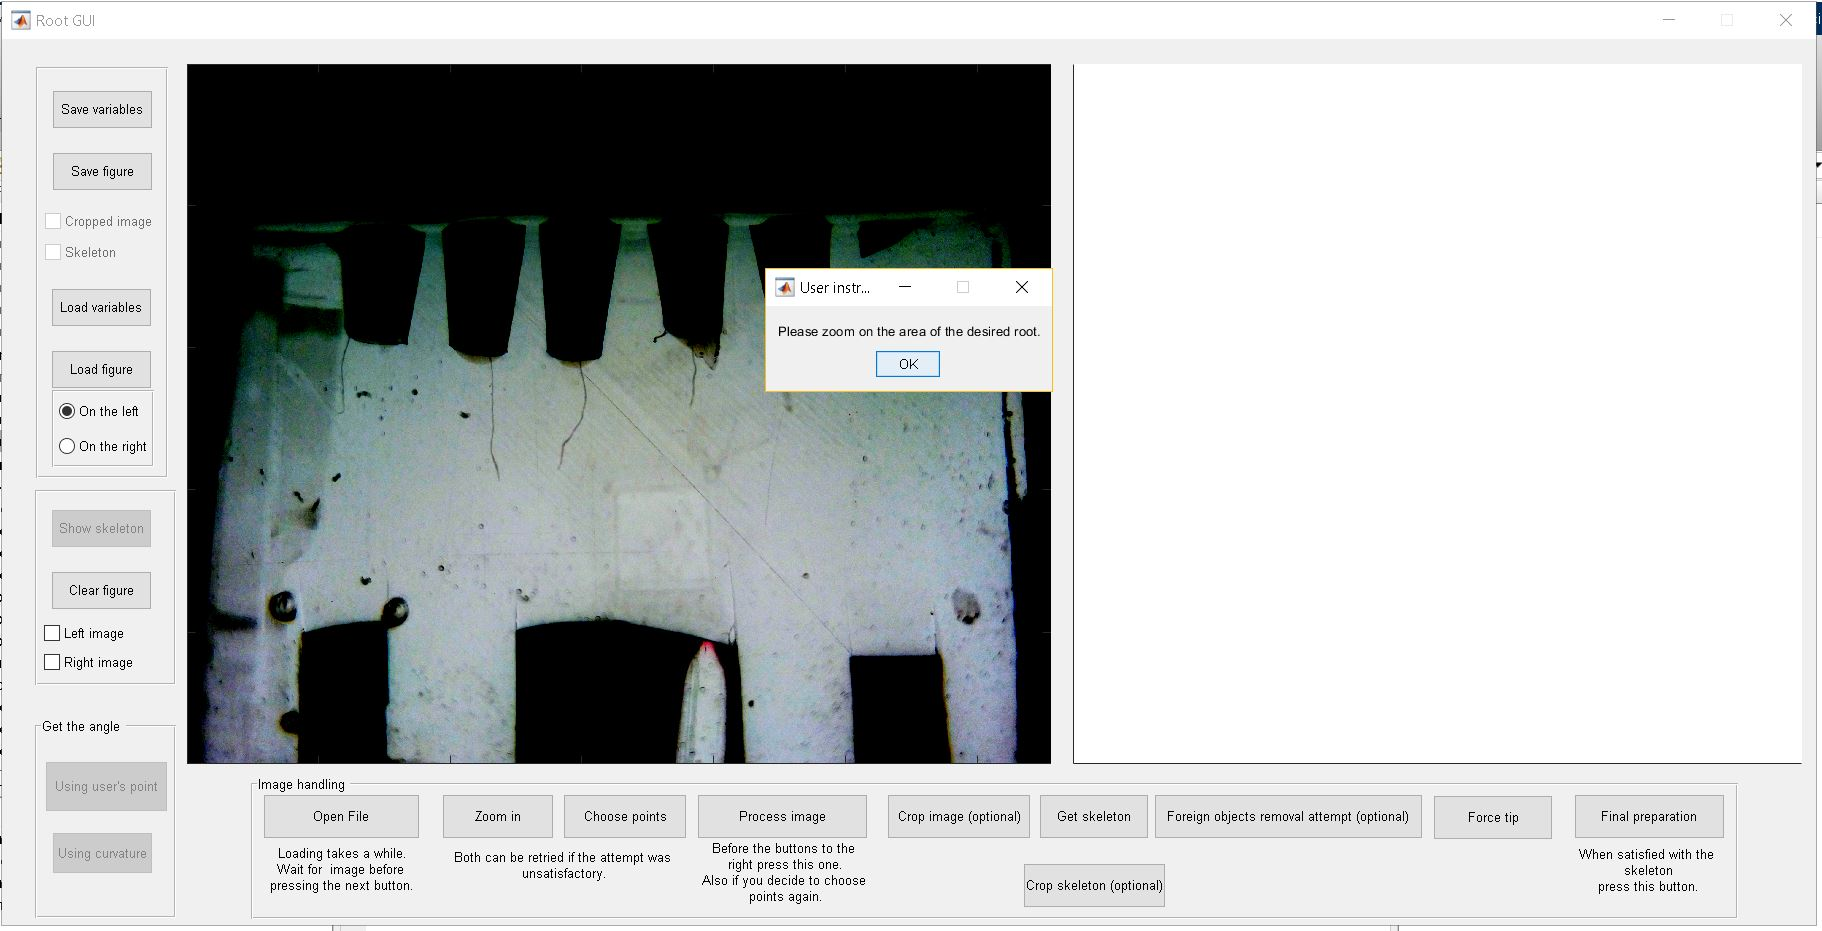
\includegraphics[width=\textwidth]{../Figures/manual/step4.jpg}
 	\caption{Prompt to zoom in on the dedired root}
 	\label{fig:img7}
\end{figure} 	
 
\begin{figure}[H]
  	\centering
  	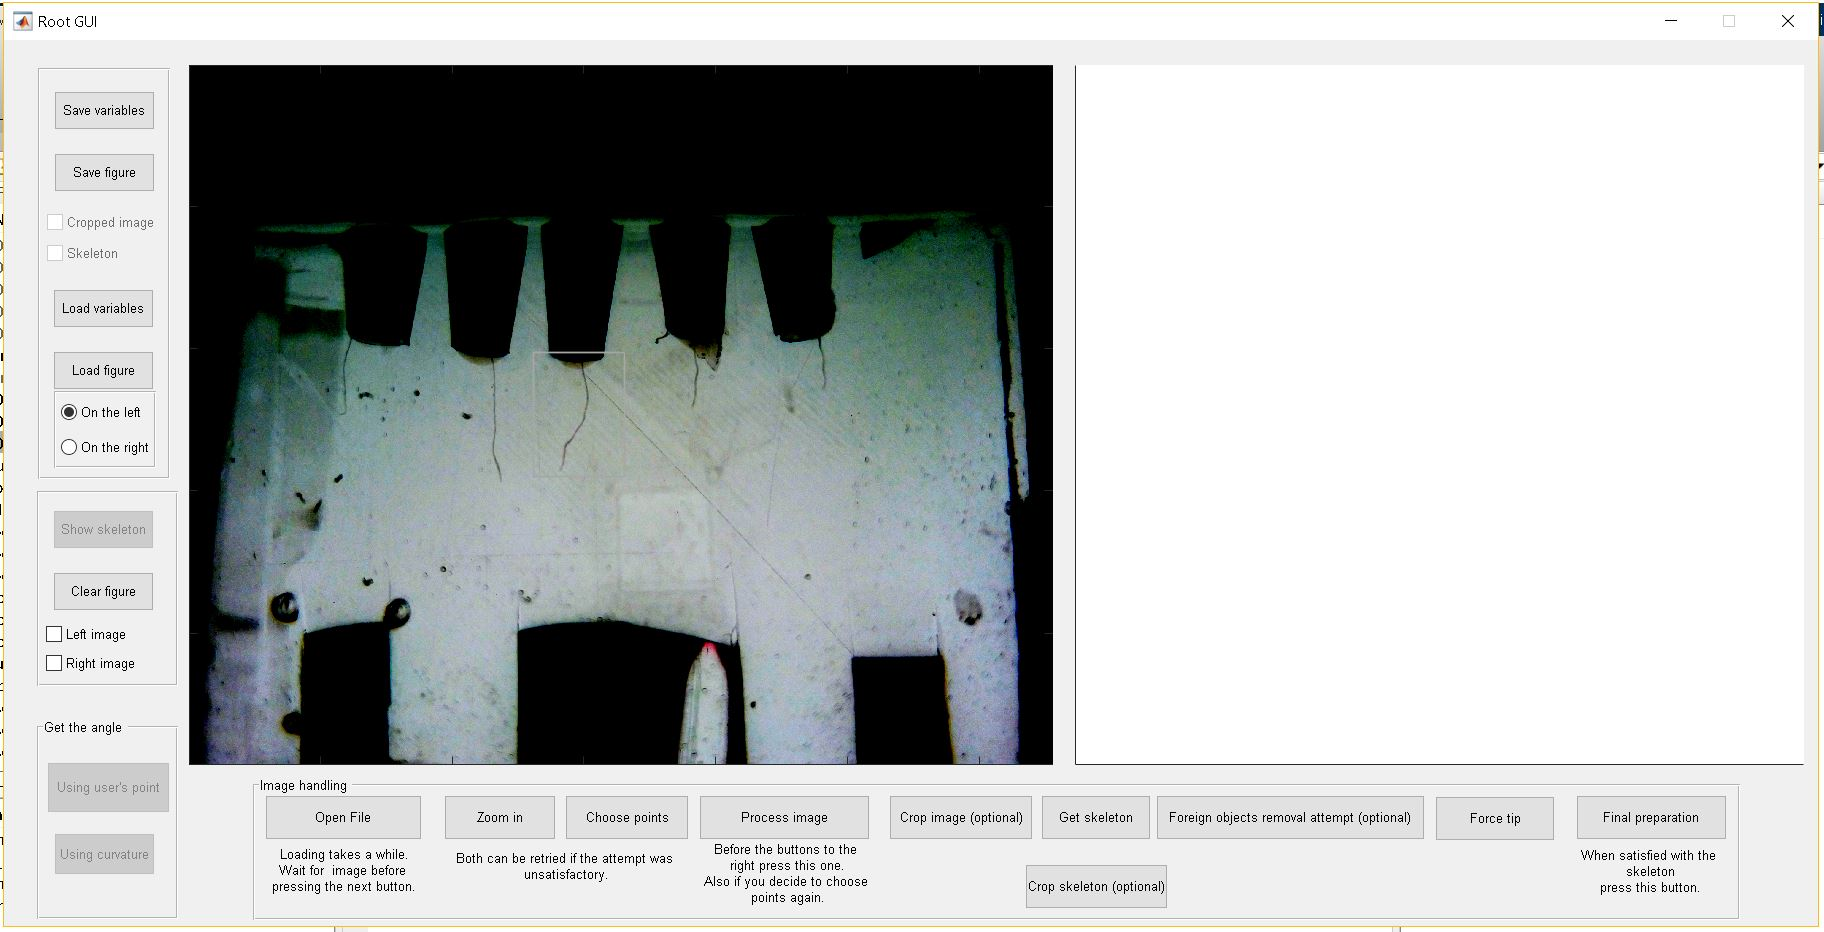
\includegraphics[width=\textwidth]{../Figures/manual/step5.jpg}
  	\caption{Drawing a rectangle around the desired root}
  	\label{fig:img8}
\end{figure}
  
Now that that's done, we want to choose points to give our program some data so that it will be able to pre-process the image.
Click the \textit{Choose points} button and follow the instructions that will appear on the screen: Choose as many points as the instruction tells you, and on the last step only the tip of the root (see figures \ref{fig:img9})

\begin{figure}[H]
	\centering
	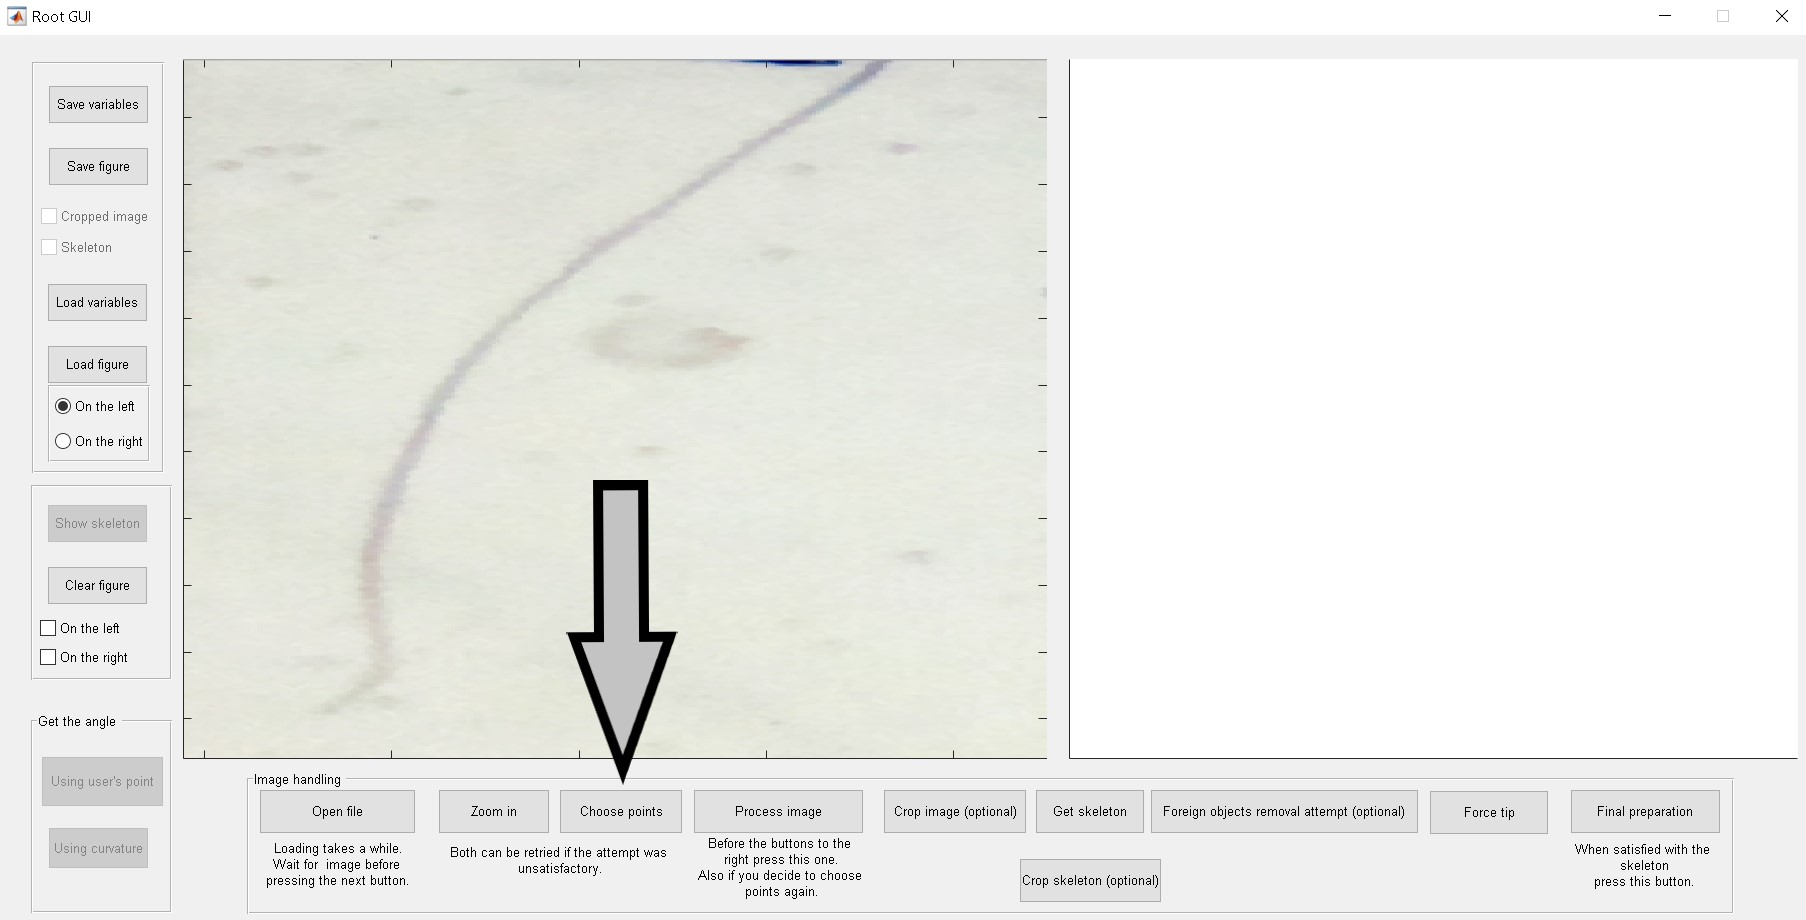
\includegraphics[width=\textwidth]{../Figures/manual/step6.jpg}
	\caption{Step 3 in the \textit{RootSkel} pipeline: Choosing points along the root}
	\label{fig:img9}
\end{figure}

\begin{figure}[H]
	\centering
	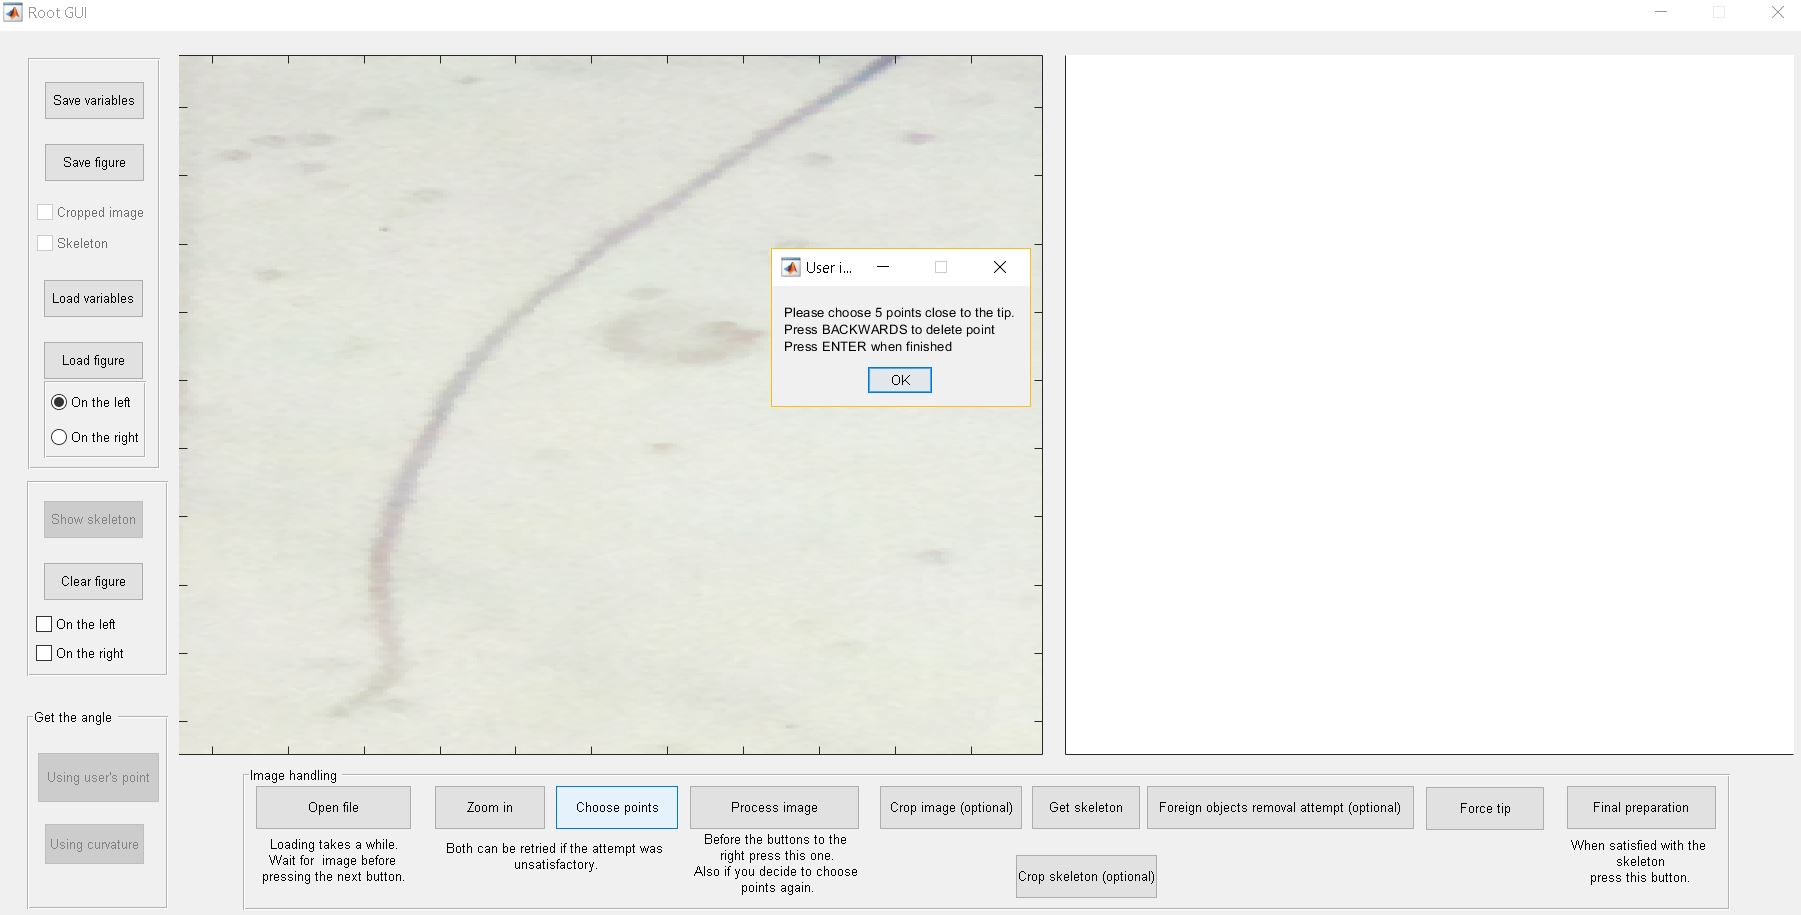
\includegraphics[width=\textwidth]{../Figures/manual/step7.jpg}
	\caption{Prompt to choose 5 points close to the tip of the root}
	\label{fig:img10}
\end{figure}

\begin{figure}[H]
	\centering
	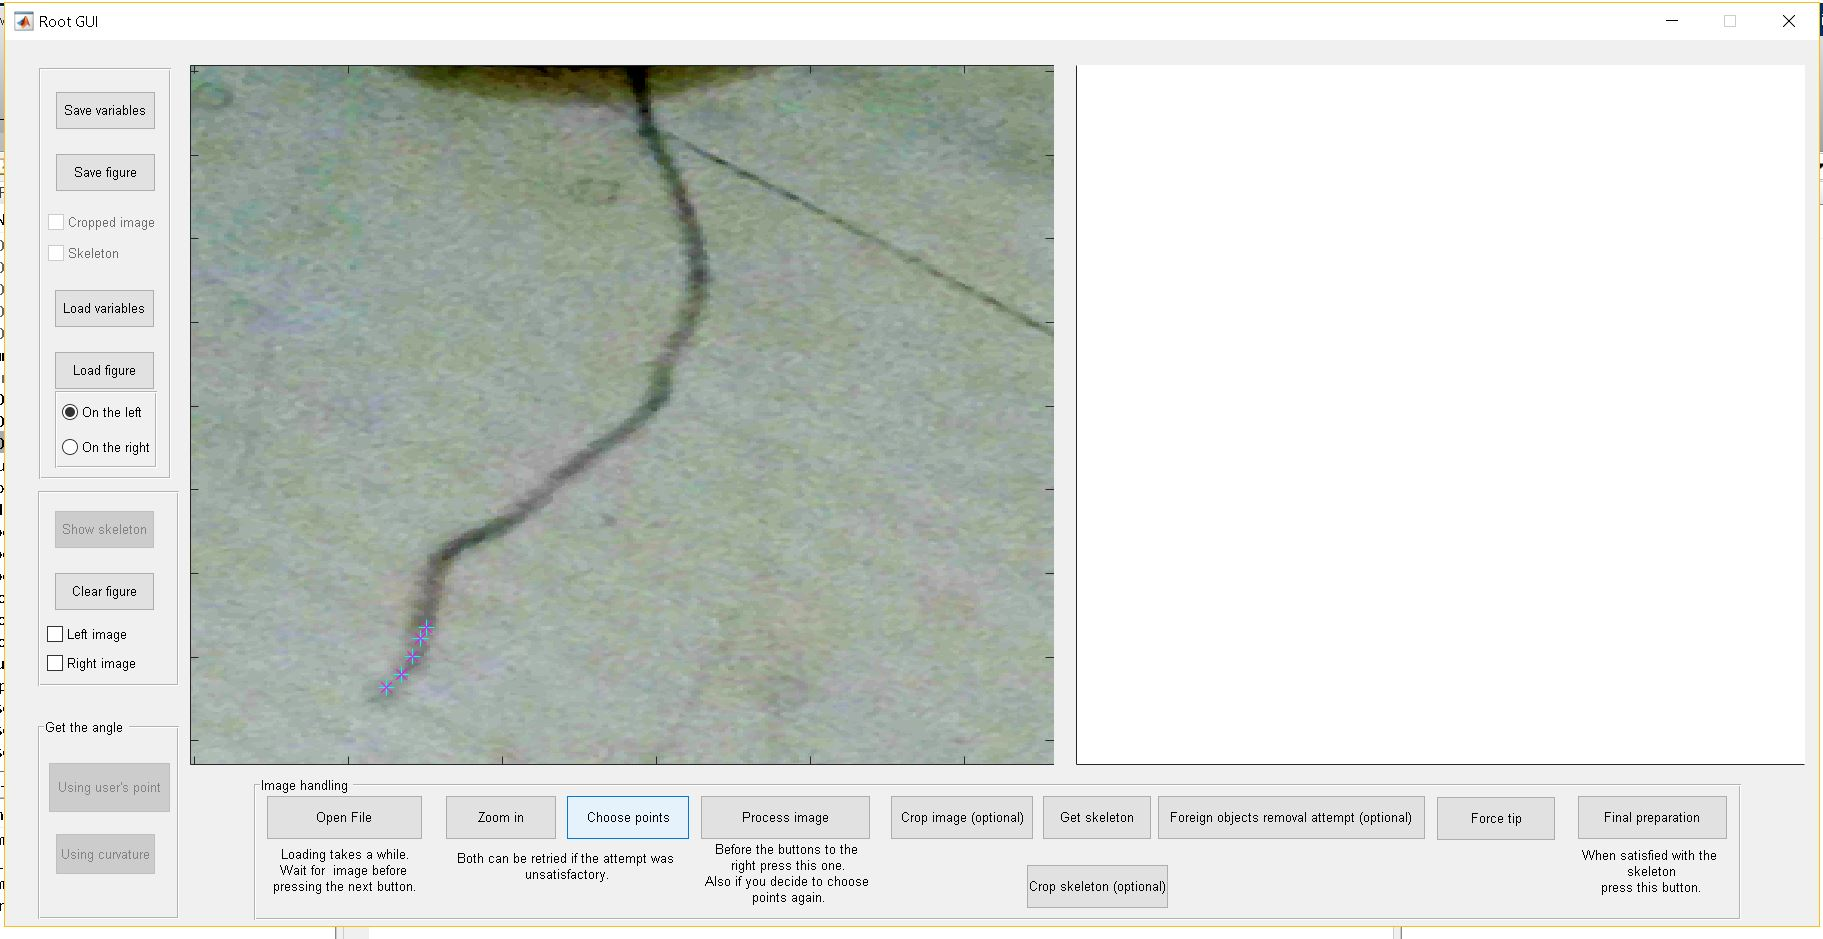
\includegraphics[width=\textwidth]{../Figures/manual/step8.jpg}
	\caption{After choosing the 5 points close to the tip}
	\label{fig:img11}
\end{figure}

\begin{figure}[H]
	\centering
	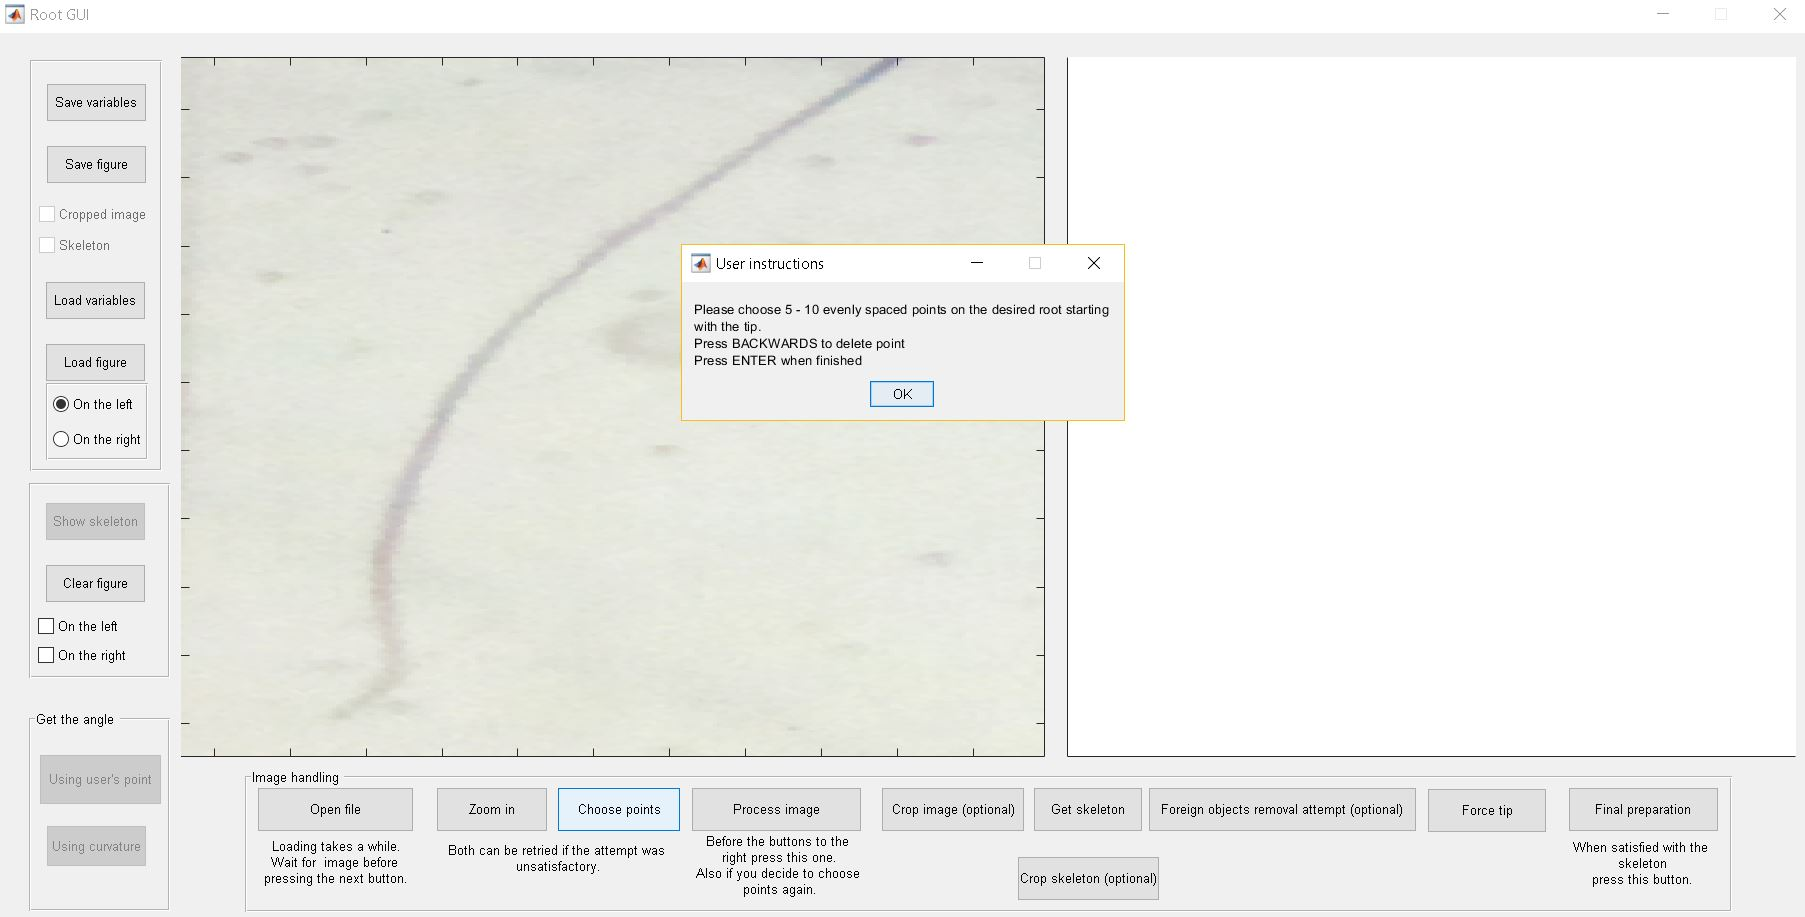
\includegraphics[width=\textwidth]{../Figures/manual/step9.jpg}
	\caption{Prompt to choose 5-10 points on the root starting with the tip}
	\label{fig:img12}
\end{figure}

\begin{figure}[H]
	\centering
	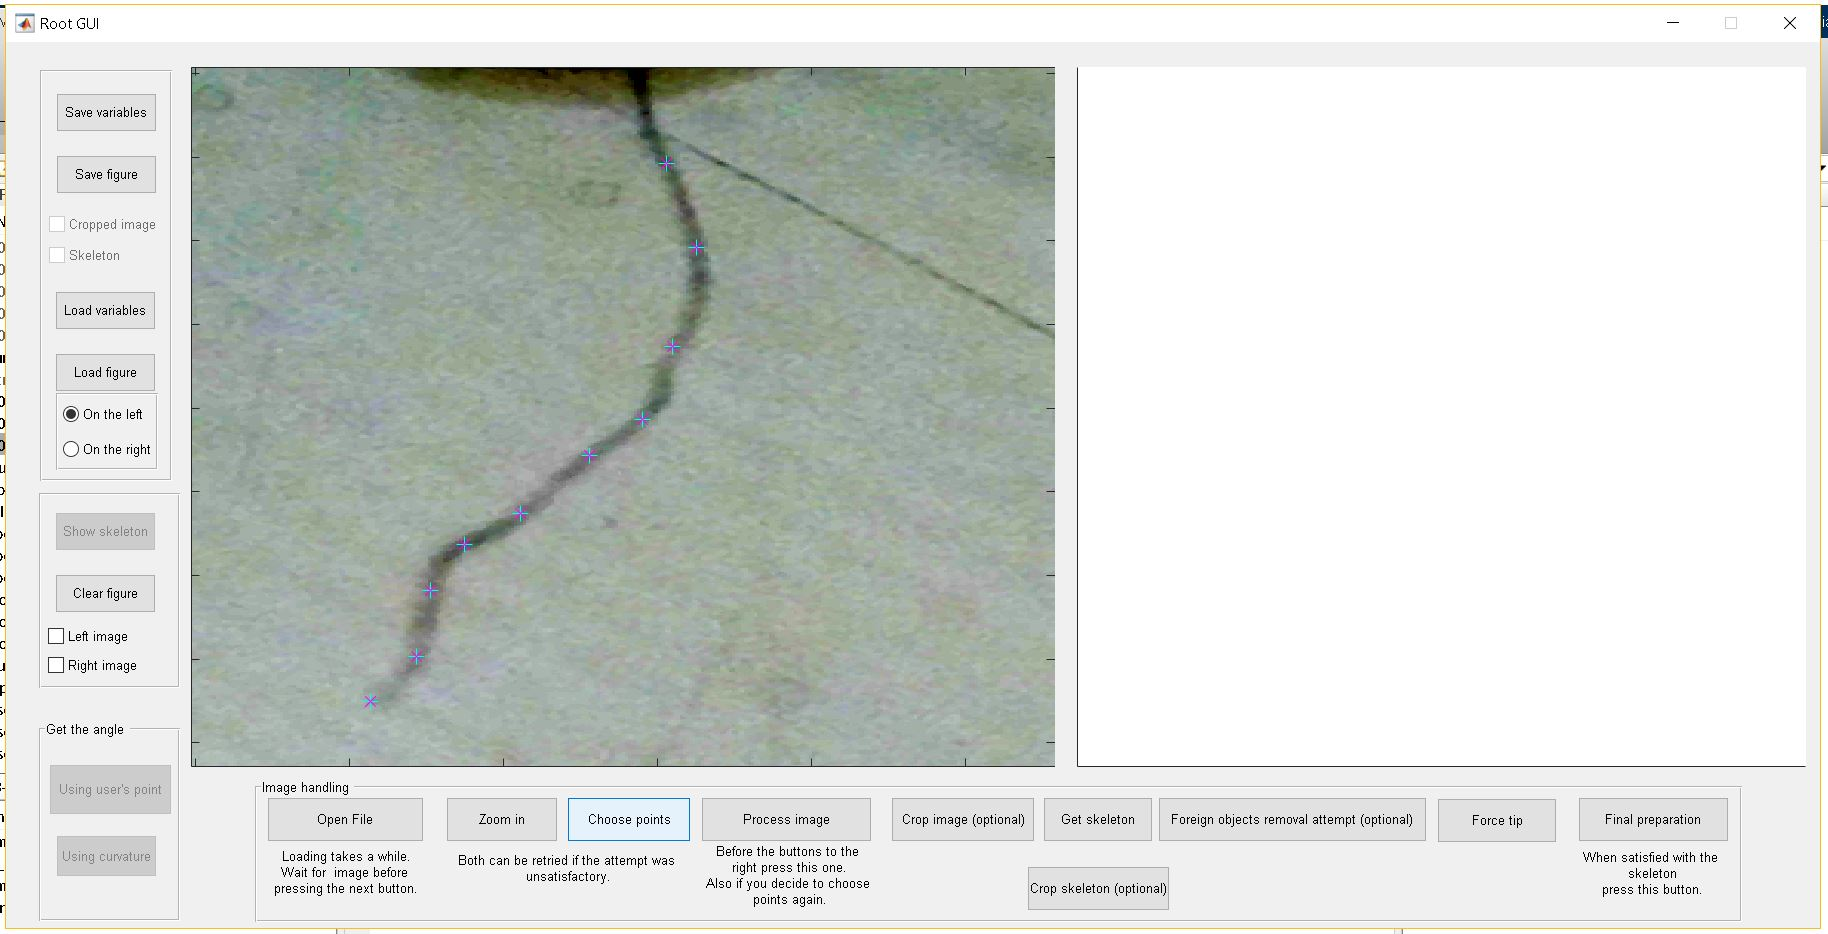
\includegraphics[width=\textwidth]{../Figures/manual/step10.jpg}
	\caption{After choosing the 5-10 points on the root}
	\label{fig:img13}
\end{figure}

\begin{figure}[H]
	\centering
	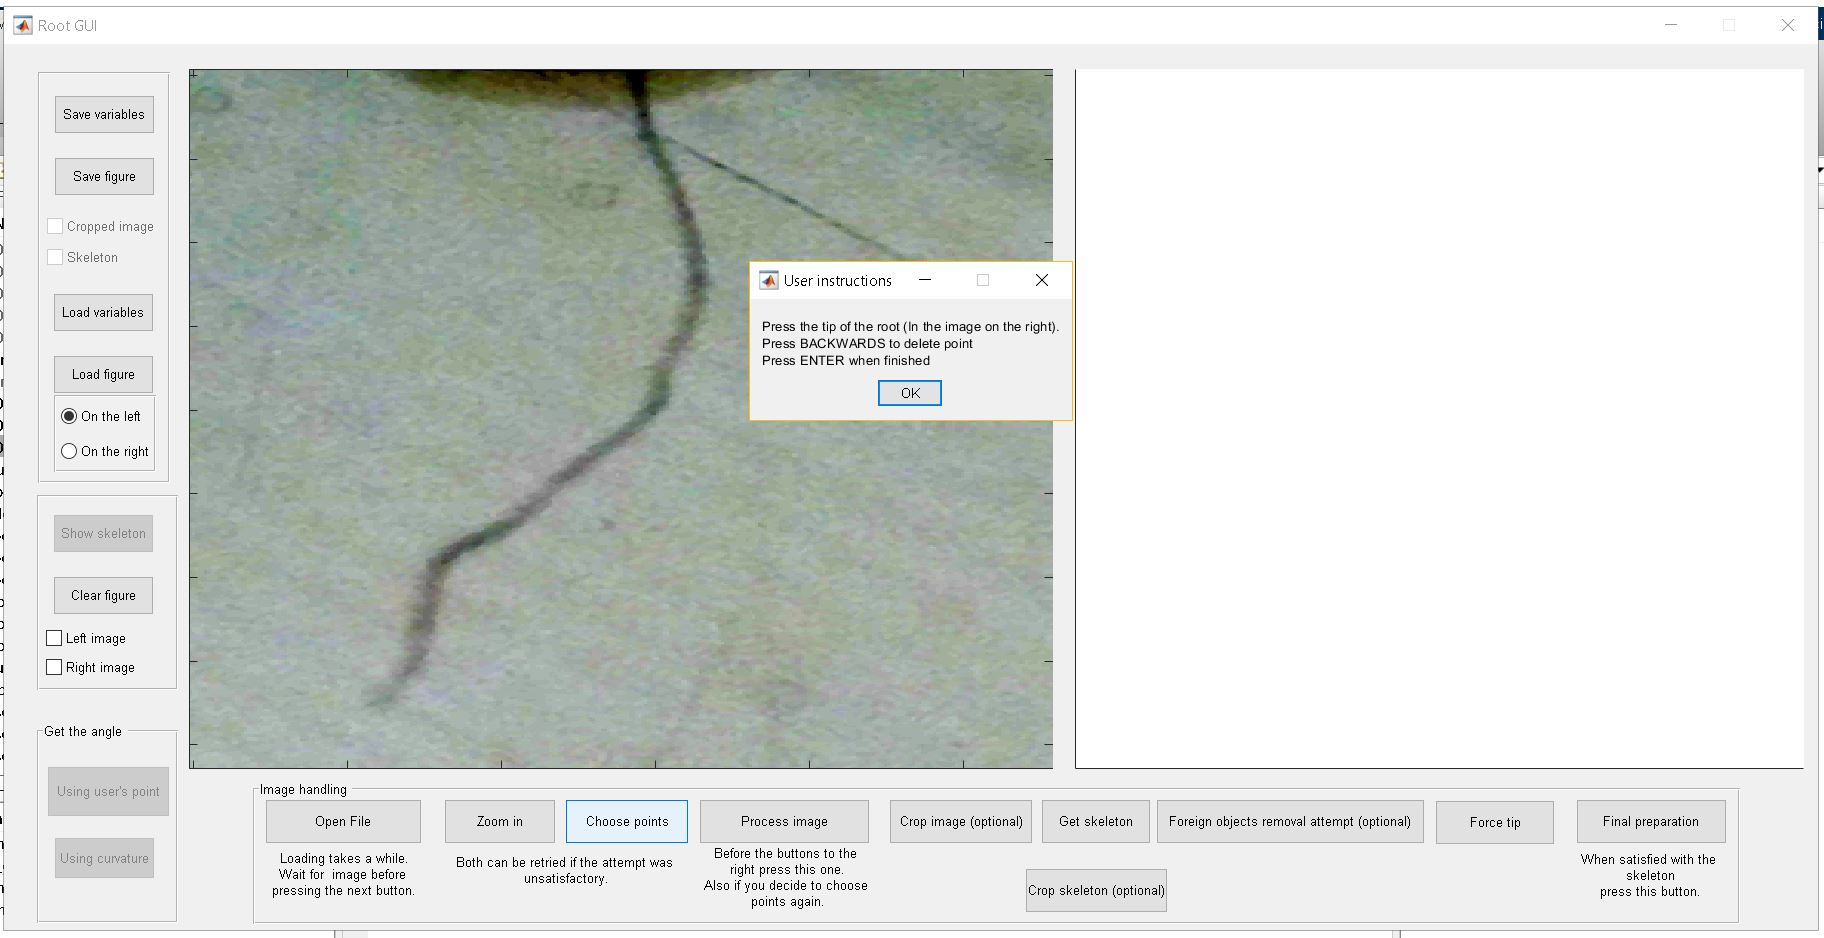
\includegraphics[width=\textwidth]{../Figures/manual/step11.jpg}
	\caption{Prompt to press the tip of the root in the image on the RHS}
	\label{fig:img14}
\end{figure}

\begin{figure}[H]
	\centering
	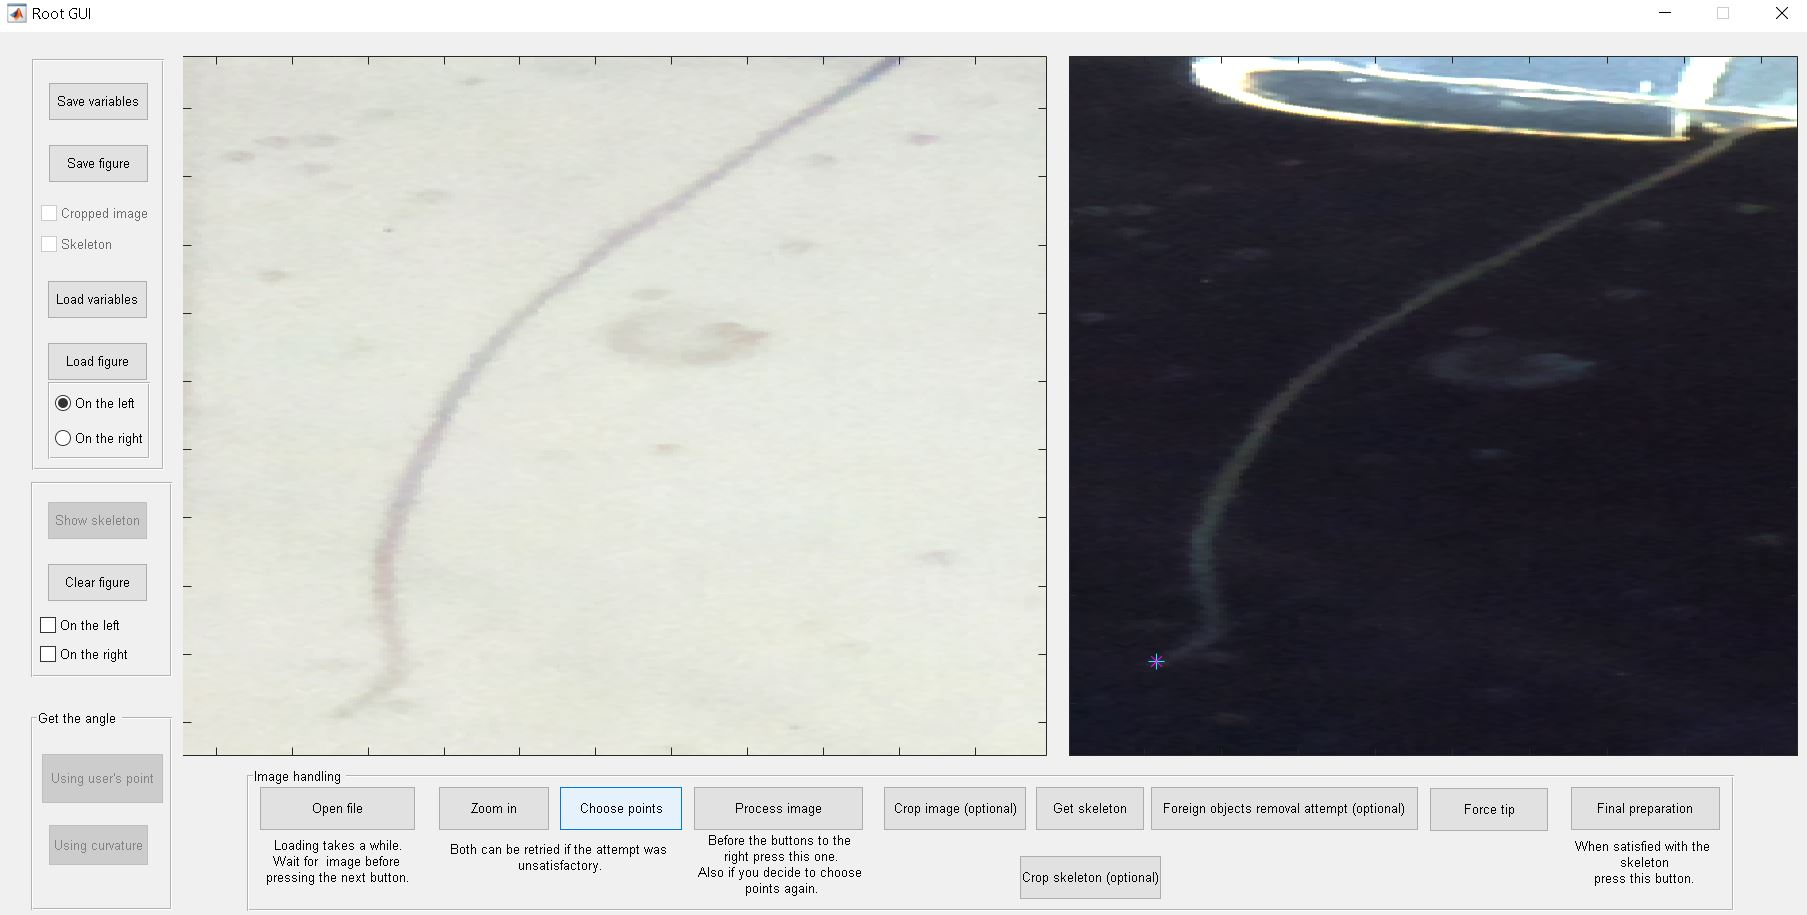
\includegraphics[width=\textwidth]{../Figures/manual/step12.jpg}
	\caption{After choosing the tip of the root}
	\label{fig:img15}
\end{figure}

Now that we did the work to feed in some points, it's time to let the program do its part. Click on the \textit{Process image} buton to make the program preprocess the image for the next part of getting the skeleton (see figure \ref{fig:img16}).

\begin{figure}[H]
	\centering
	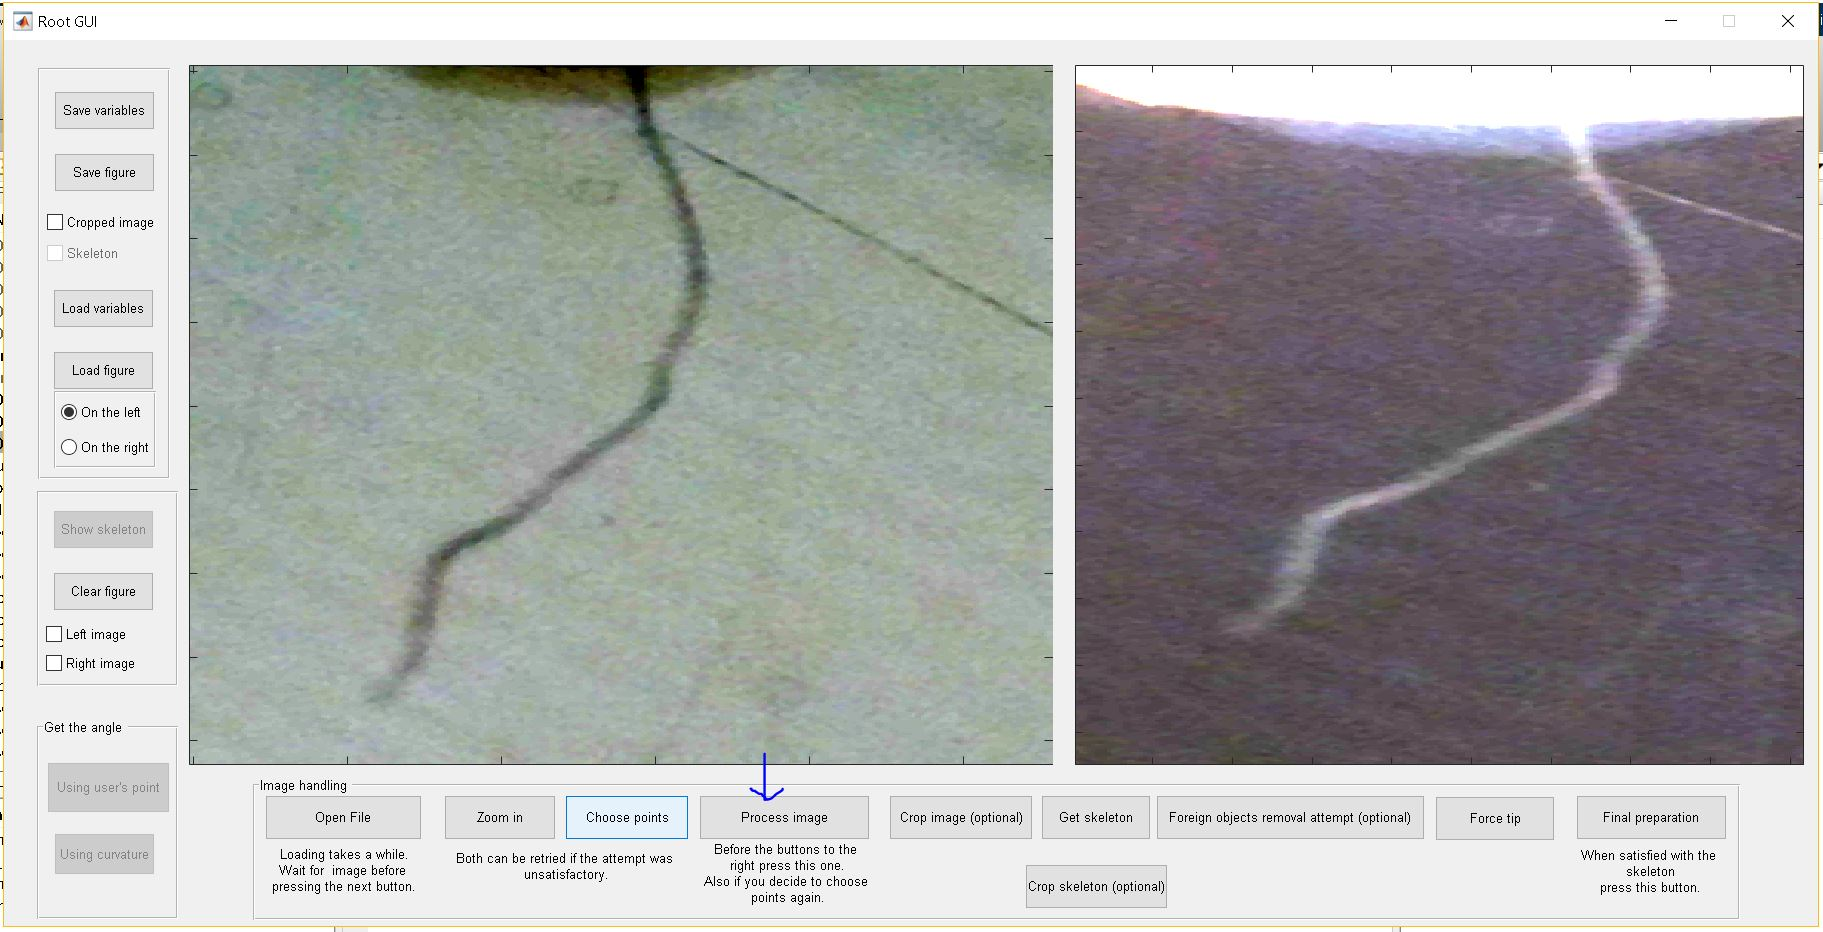
\includegraphics[width=\textwidth]{../Figures/manual/step13.jpg}
	\caption{Step 4 in the \textit{RootSkel} pipeline: Processing the image}
	\label{fig:img16}
\end{figure}

A message will pop up when the processing is done (see figure \ref{fig:img17}).
\begin{figure}[H]
	\centering
	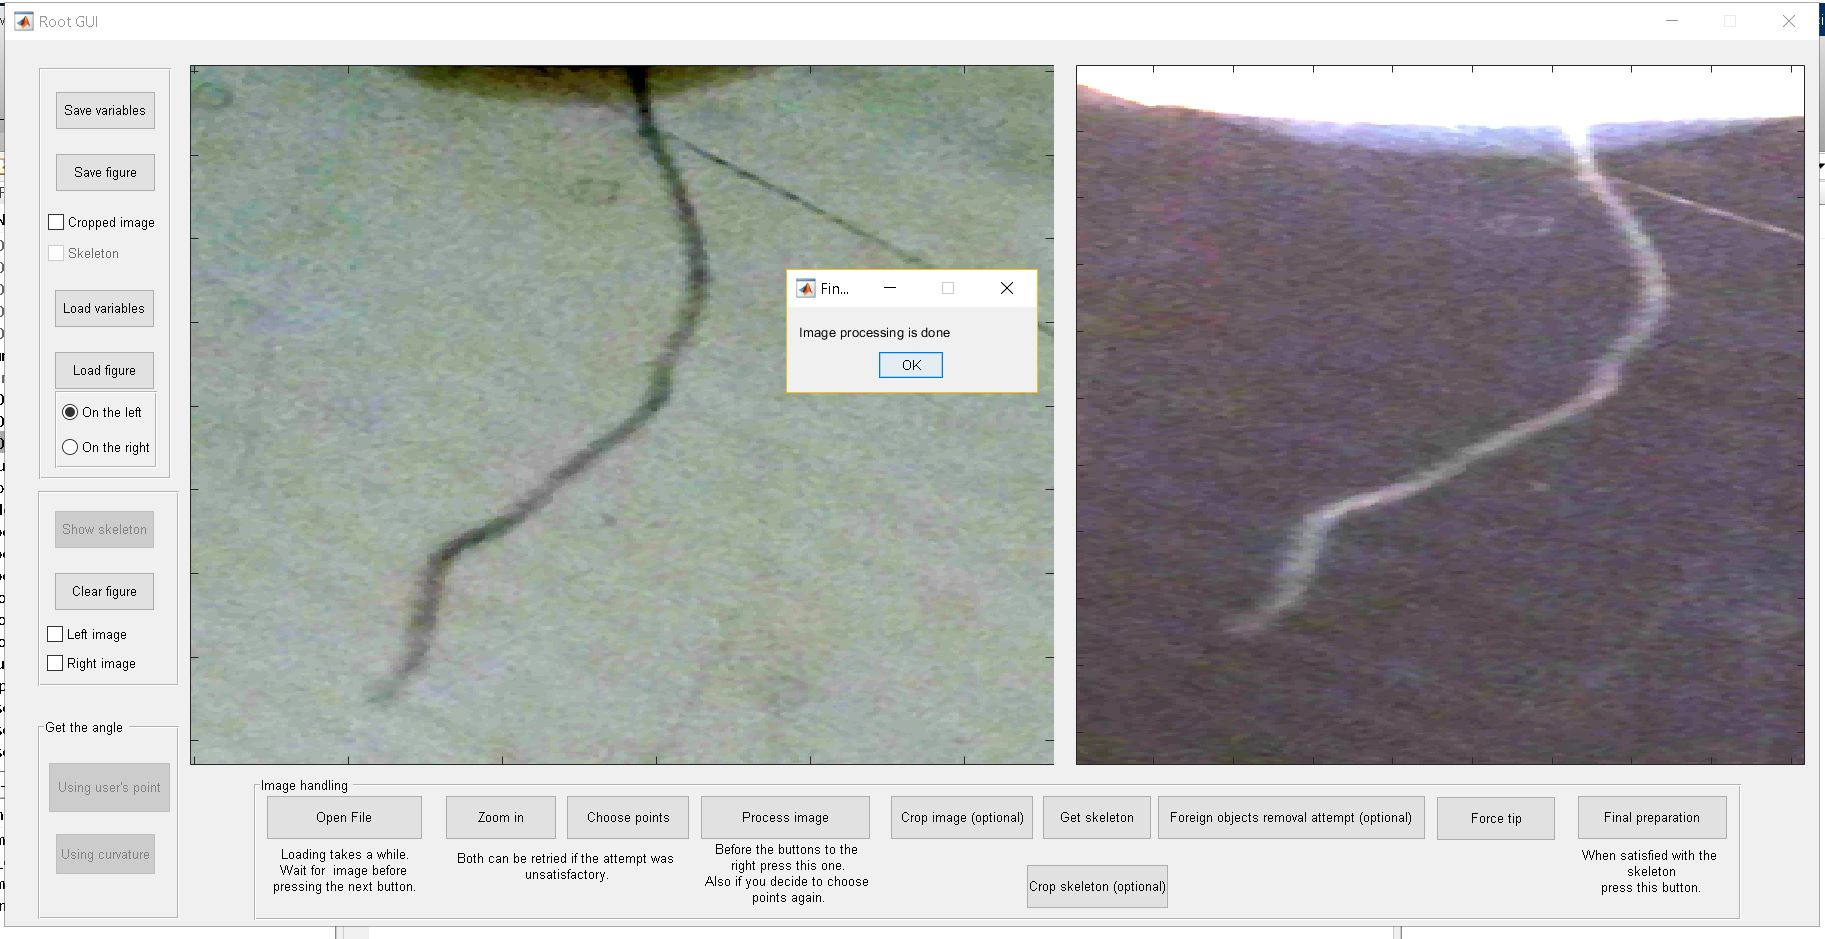
\includegraphics[width=\textwidth]{../Figures/manual/step14.jpg}
	\caption{After the processing is done}
	\label{fig:img17}
\end{figure}

Now we need to click the \textit{Get skeleton} button (see figure \ref{fig:img18}) to get the result in the image on the RHS (see figure \ref{fig:img19}).

\begin{figure}[H]
	\centering
	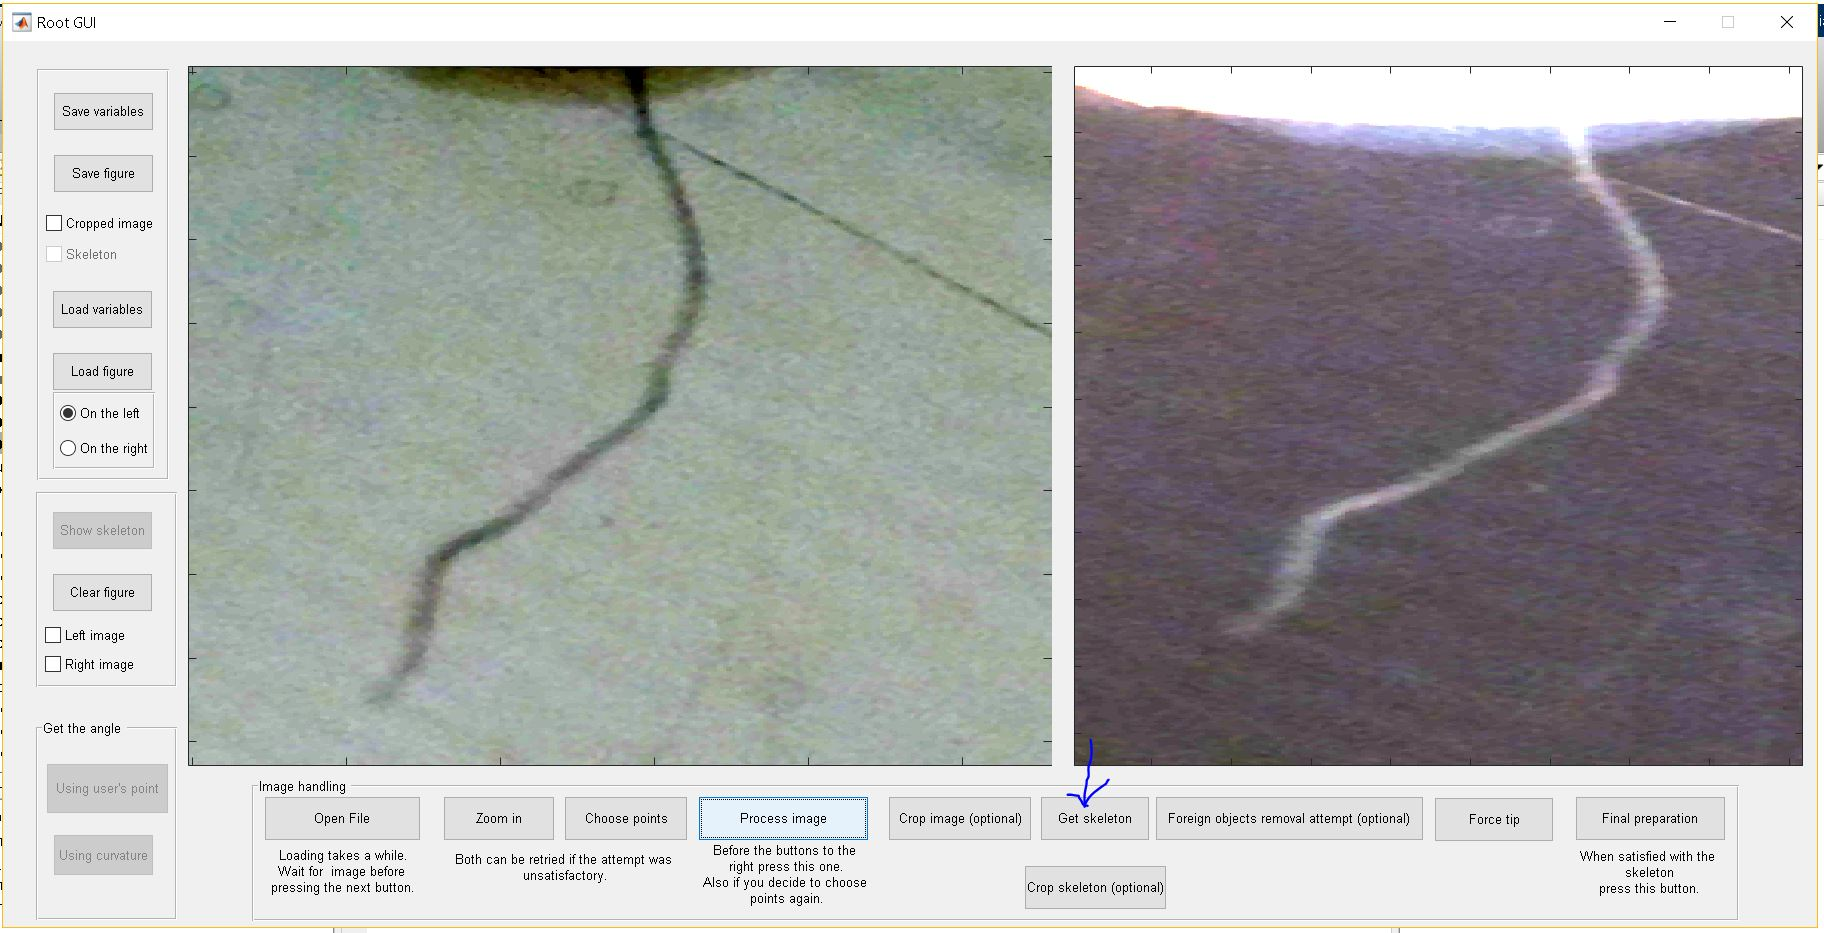
\includegraphics[width=\textwidth]{../Figures/manual/step15.jpg}
	\caption{Step 5 in the \textit{RootSkel} pipeline: Getting the skeleton}
	\label{fig:img18}
\end{figure}

\begin{figure}[H]
	\centering
	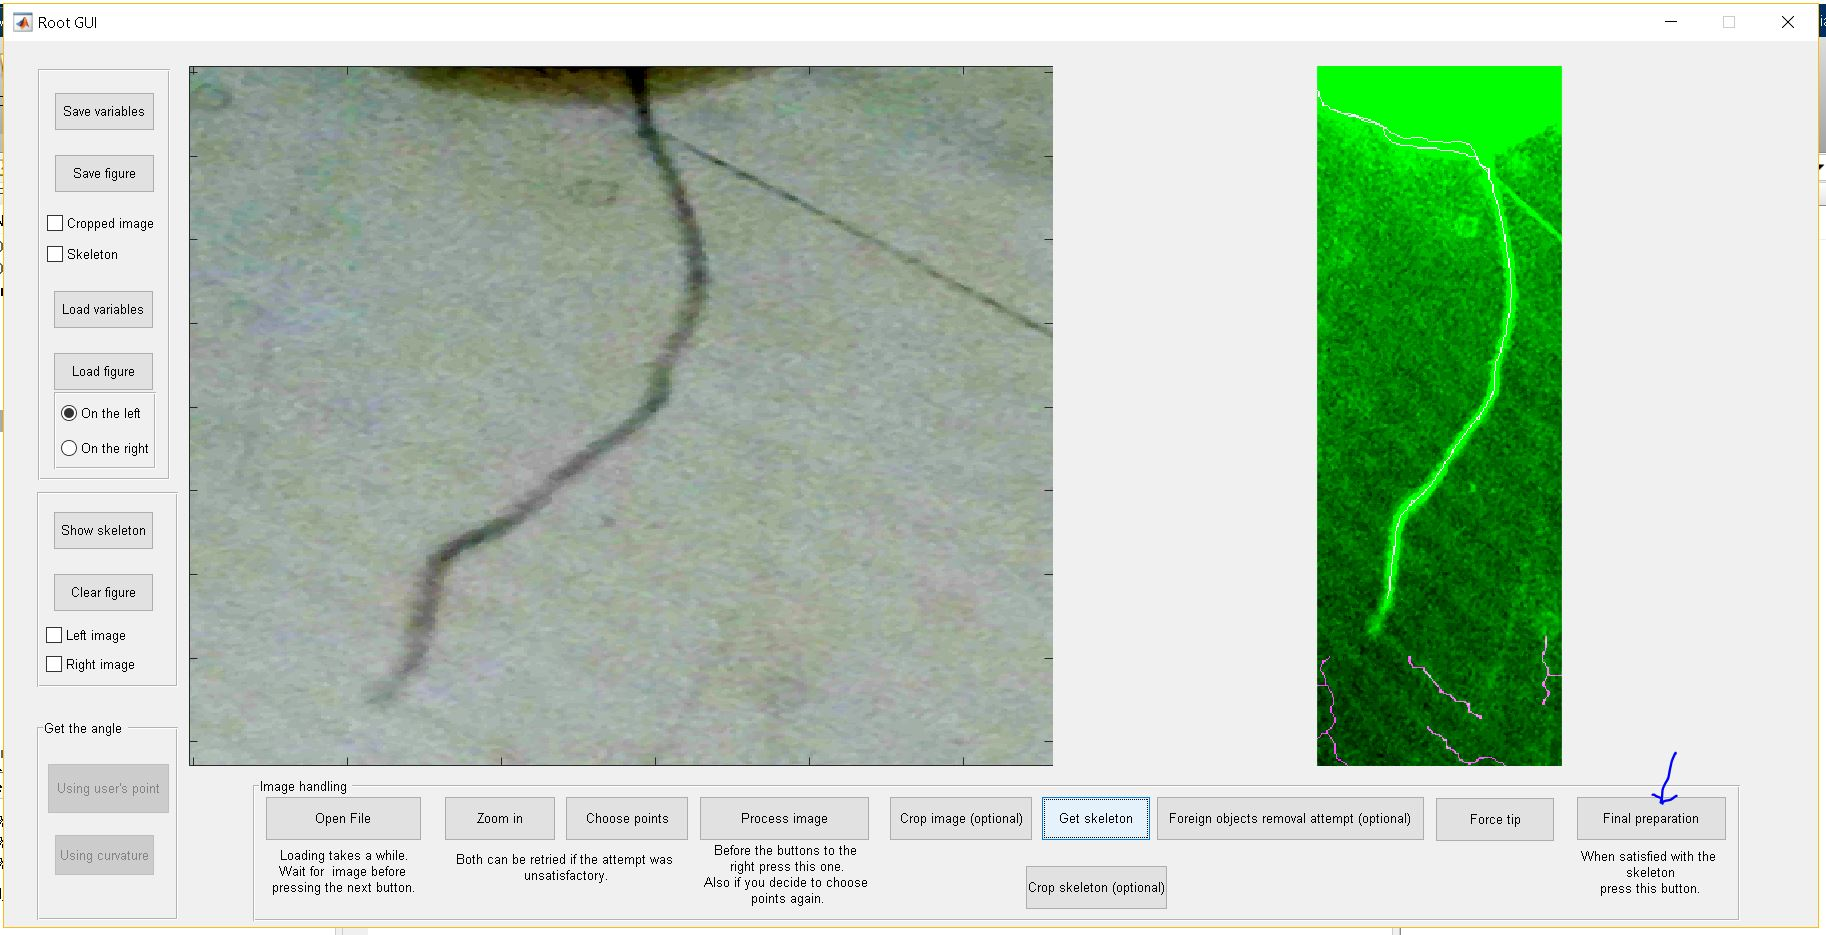
\includegraphics[width=\textwidth]{../Figures/manual/step16.jpg}
	\caption{Getting the skeleton}
	\label{fig:img19}
\end{figure}

Now we've got ourselves a root (it's not perfect, but we'll get into optional improvement steps in a minute), so it's time to get on with it. 
Let's now click the \textit{Final preparation} button and then click 'No' when presented the chance (we will get into the alternative option later) to get ready for the angle calculation (see figures \ref{fig:img19} and \ref{fig:img20}).

\begin{figure}[H]
	\centering
	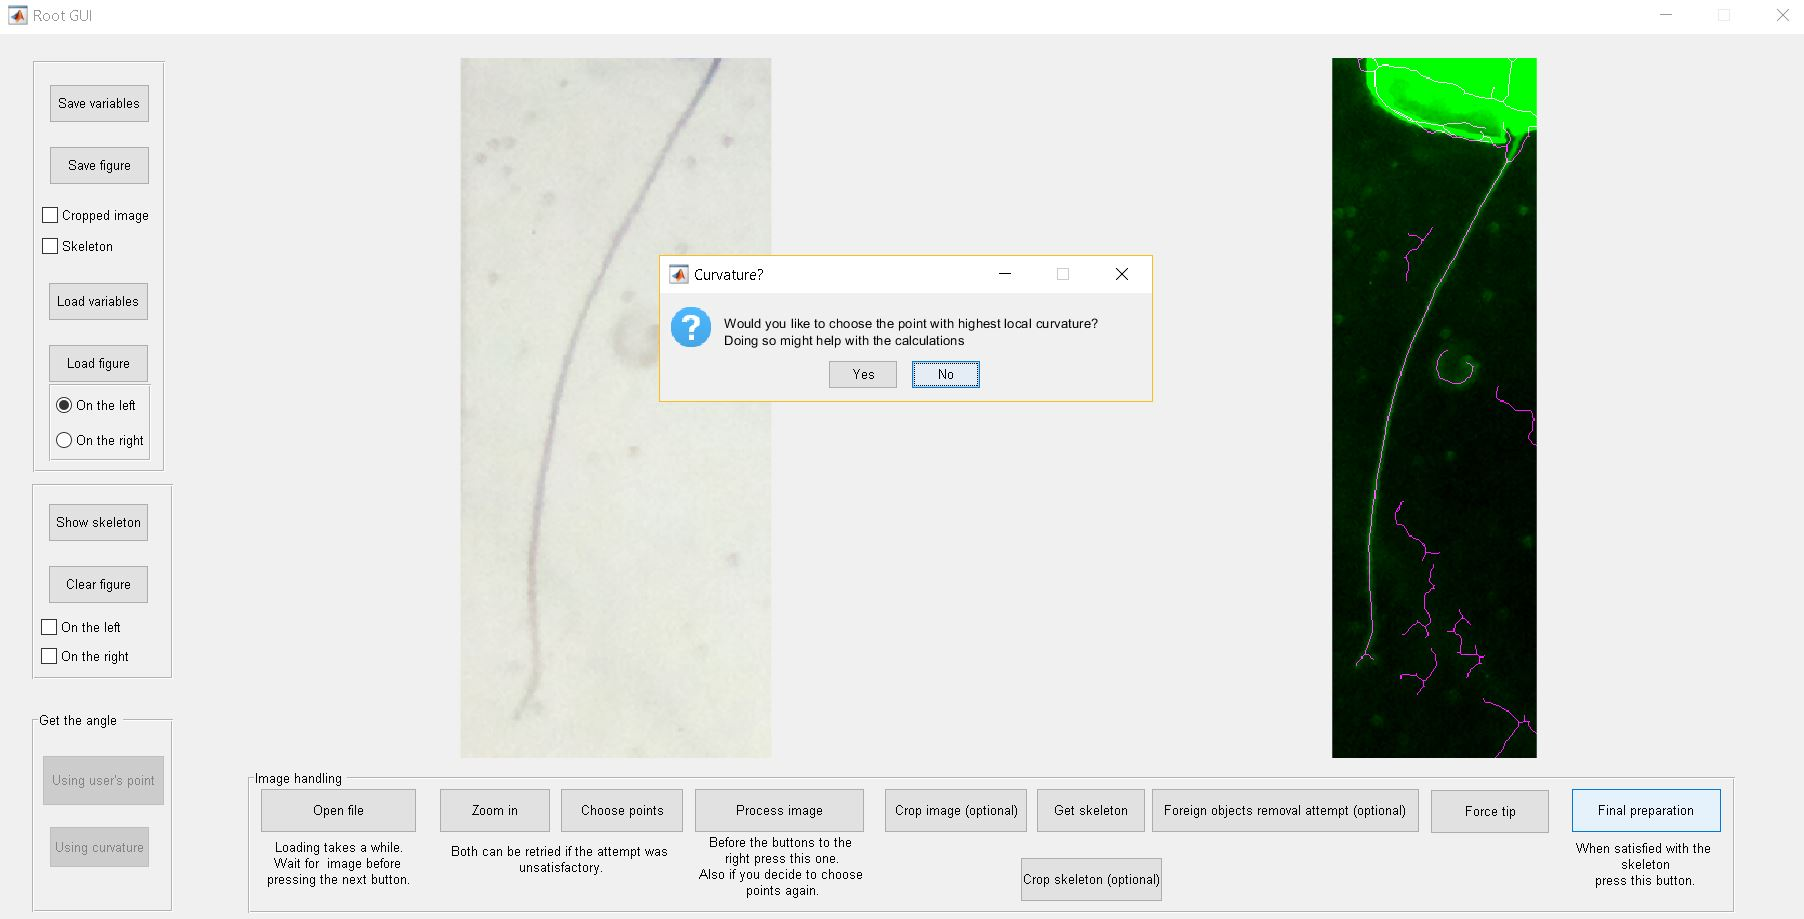
\includegraphics[width=\textwidth]{../Figures/manual/step17.jpg}
	\caption{Clicking 'No' when asked to choose the point of highest local (mean) curvature}
	\label{fig:img20}
\end{figure}

Here we are, the last step before we get an angle for our root. 
All that is left to do, is clicking one of the angle calculations buttons.
Now, since we clicked 'No' in the previous step, we only get the \textit{Using curvature} button, so click this one (see figure \ref{fig:img21}).
Later in the manual, we will go over the option to include a point of local maximum curvature by the user. 
Now you will get the angle and then you will be asked to enter the root number (unless you clicked on one of the other buttons requiring this information, i.e. \textit{Save variables} and \textit{Save figures}. More on that later.) (see figures \ref{fig:img22} and \ref{fig:img23}).

\begin{figure}[H]
	\centering
	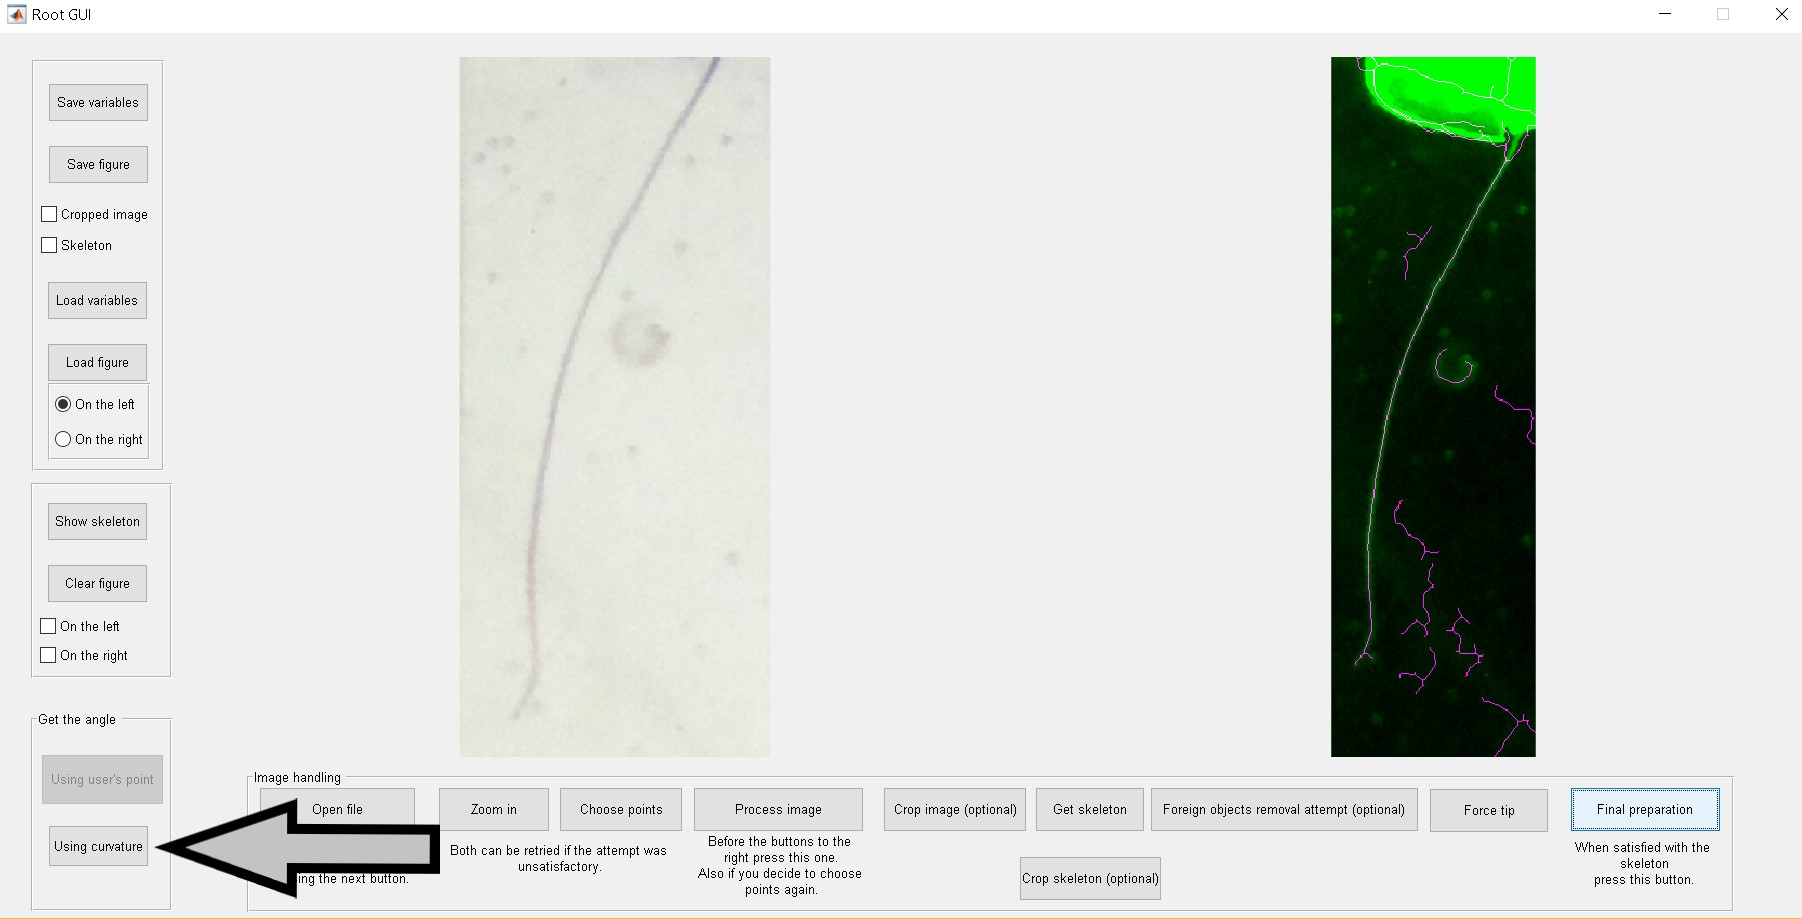
\includegraphics[width=\textwidth]{../Figures/manual/step18.jpg}
	\caption{Step 6 in the \textit{RootSkel} pipeline: Clicking \textit{Using curvature} for the angle computation}
	\label{fig:img21}
\end{figure}

\begin{figure}[H]
	\centering
	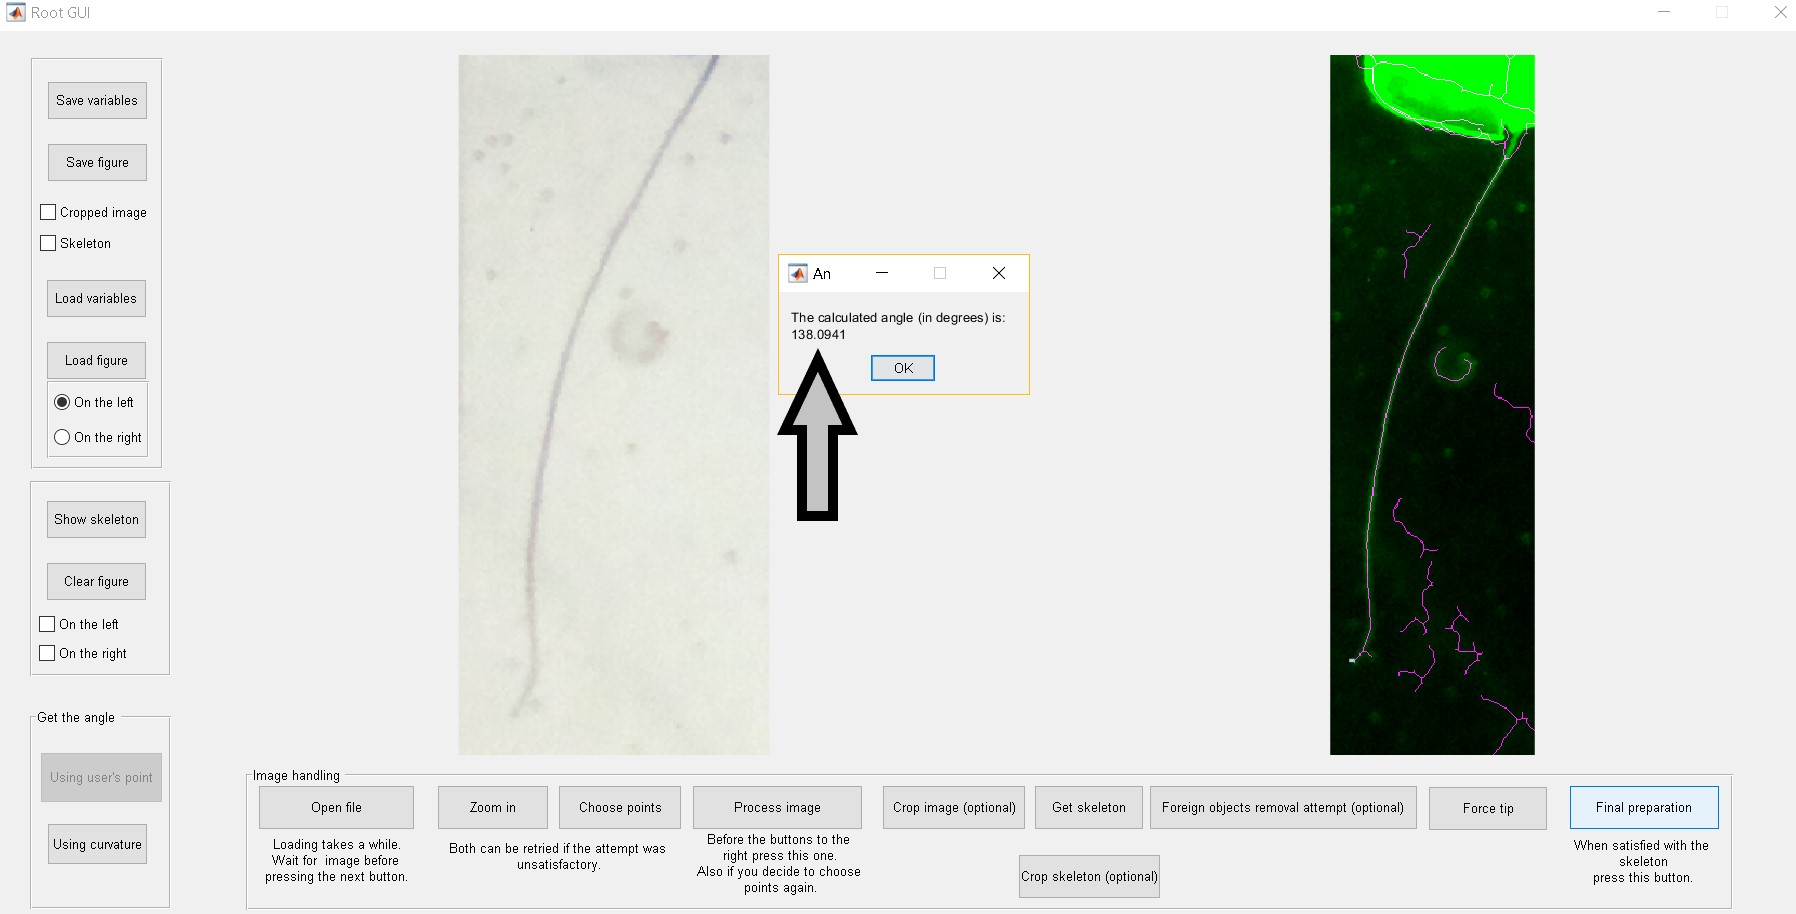
\includegraphics[width=\textwidth]{../Figures/manual/step19.jpg}
	\caption{Getting the computed the angle}
	\label{fig:img22}
\end{figure}

\begin{figure}[H]
	\centering
	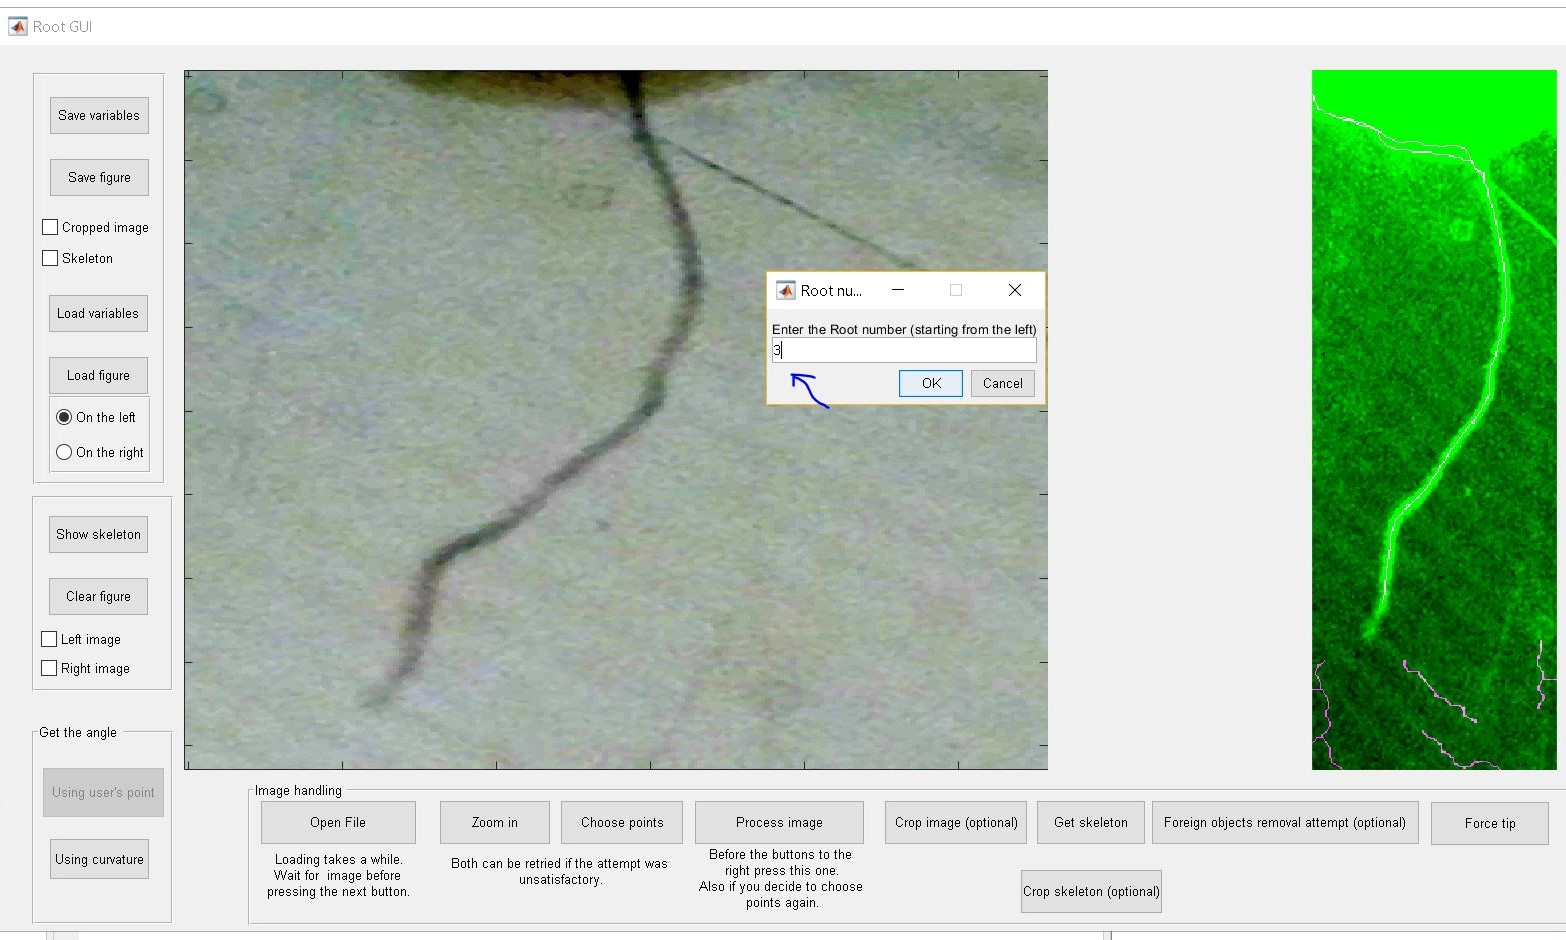
\includegraphics[width=\textwidth]{../Figures/manual/step20.jpg}
	\caption{Entering the root number (starting from the LHS)}
	\label{fig:img23}
\end{figure}

And that's it. At least without any optional steps. To the optional features we will get later in the manual. 


%----------------------------------------------------------------------------------------
\subsection{Saving}

Now say you want to save the data you got after the \textit{Final preparation}. That's what the save buttons are for.
We'll start with \textit{Save variables} (see figure \ref{fig:img24}).

\begin{figure}[H]
	\centering
	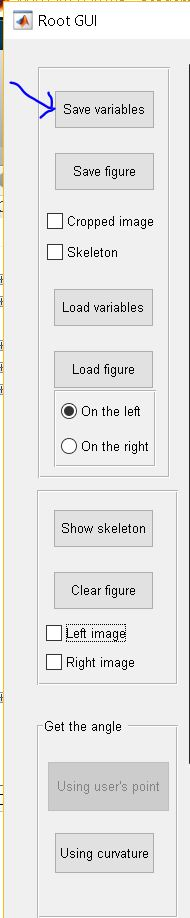
\includegraphics[width=0.3\textwidth]{../Figures/manual/save1.jpg}
	\caption{Saving all relevant variables}
	\label{fig:img24} 
\end{figure}

After you have clicked the \textit{Save variables} button, you will be prompted to give the program the root number if you haven't done so yet (see figure \ref{fig:img23}).
Otherwise you will see the following on your screen:

\begin{figure}[H]
	\centering
	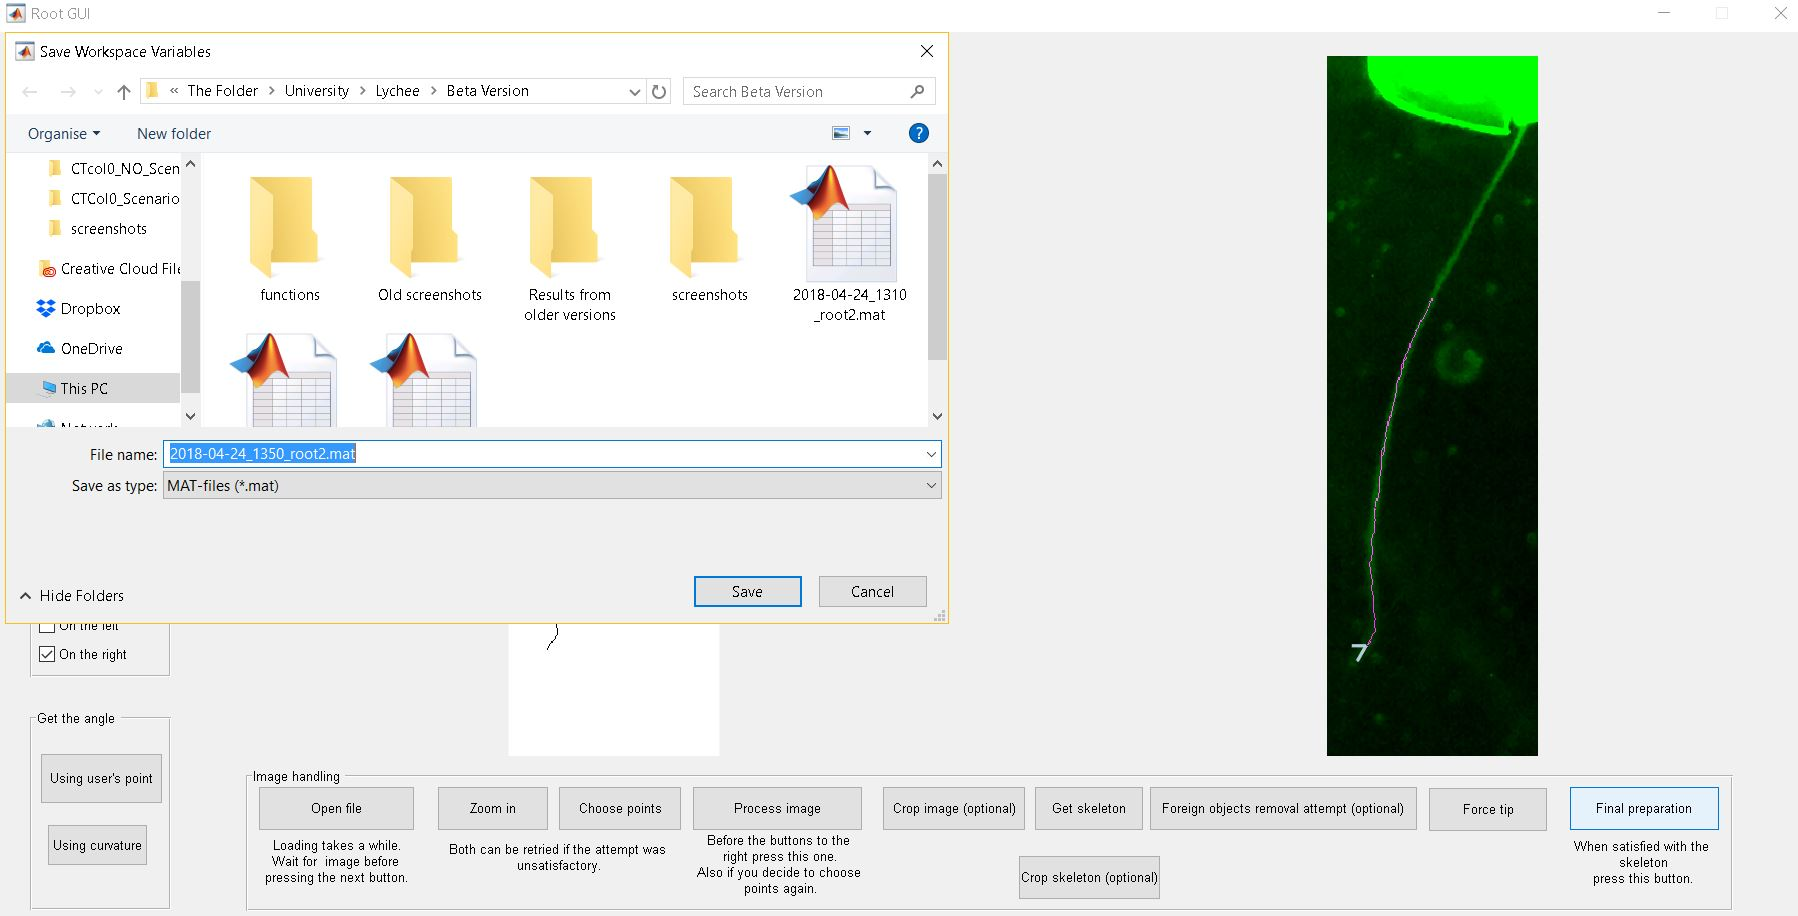
\includegraphics[width=\textwidth]{../Figures/manual/save2.jpg}
	\caption{Saving the relevant variables in a .mat file}
	\label{fig:img25}
\end{figure}

As you can see, the default name consists of the name of the original image file and the number of the root. 
So now you can save your root data in a .mat file whenever you want. You will see the .mat file in the specified location on the LHS on the screen (see figure \ref{fig:img26}).

\begin{figure}[H]
	\centering
	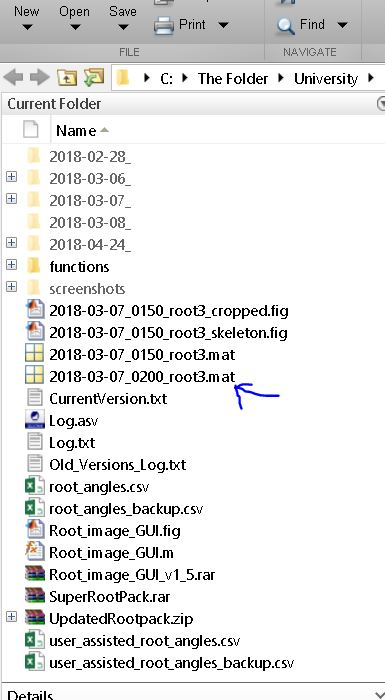
\includegraphics[width=0.5\textwidth]{../Figures/manual/save3.jpg}
	\caption{The saved .mat file with the relevant variables popping up on the LHS of the MATLAB GUI}
	\label{fig:img26}
\end{figure}

Now that we saved the variables, let's talk about saving figures. As you can see in figure \ref{fig:img27} two figures can be saved: One focused on the root, called \textit{Cropped image} (the figure on the LHS in figures \ref{fig:img15} -- \ref{fig:img18}), and the other one is the skeleton overlayed on the root, called \textit{Skeleton} (the figure on the RHS in figures \ref{fig:img19} -- \ref{fig:img23}).
You can choose to save either one of them or both.

Assume we clicked both.

\begin{figure}[H]
	\centering
	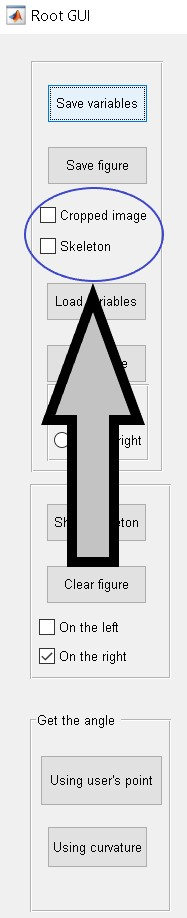
\includegraphics[width=0.3\textwidth]{../Figures/manual/save4.jpg}
	\caption{Saving of different figures: the cropped image or the skeleton}
	\label{fig:img27}
\end{figure}

Now that both are selected, the next step is to simply click on \textit{Save figure}(see figure \ref{fig:img28}).

\begin{figure}[H]
	\centering
	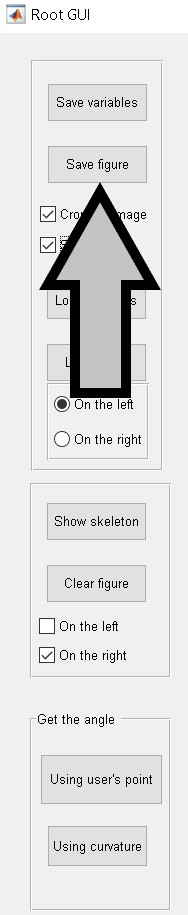
\includegraphics[width=0.3\textwidth]{../Figures/manual/save5.jpg}
	\caption{Clicking the \textit{Save figure} button}
	\label{fig:img28}
\end{figure}

After that's done, two new .fig files will appear with the appropriate end to their file name (see figure \ref{fig:img29}).

\begin{figure}[H]
	\centering
	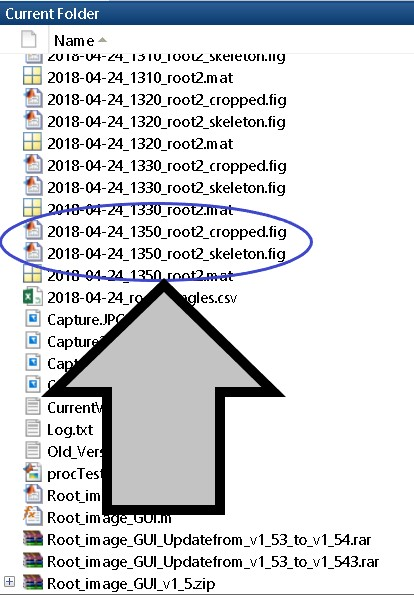
\includegraphics[width=0.6\textwidth]{../Figures/manual/save6.jpg}
	\caption{The saved .fig file(s) appearing on the LHS of the MATLAB GUI}
	\label{fig:img29}
\end{figure}


%----------------------------------------------------------------------------------------
%----------------------------------------------------------------------------------------
\subsection{Optional}

Alright, now let's get into optional things you might try to improve the skeleton.

%----------------------------------------------------------------------------------------
\subsubsection{Foreign objects removal}

First, there is a \textit{Foreign object removal} attempt, an additional cleaning step (see figure \ref{fig:img30}):

\begin{figure}[H]
	\centering
	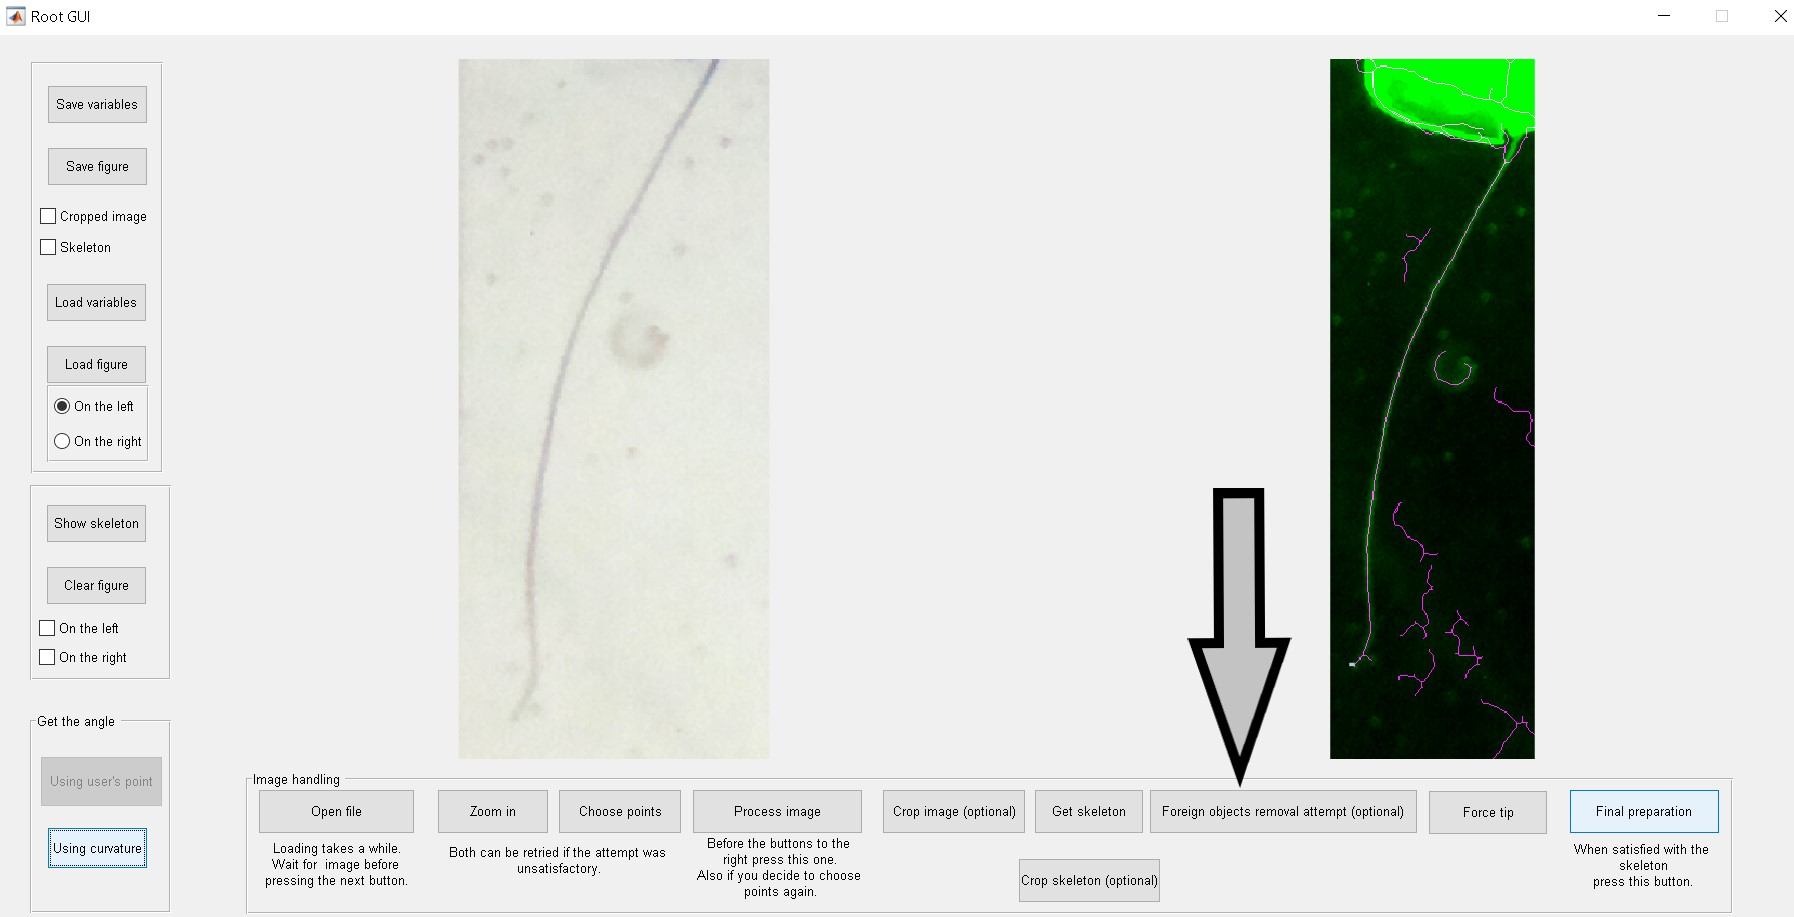
\includegraphics[width=\textwidth]{../Figures/manual/optionalA1.jpg}
	\caption{Optional step in the \textit{RootSkel} pipeline: Foreing objects removal}
	\label{fig:img30}
\end{figure}

Next you will see a message box with instructions. The basic thing is, the more times you press 'Yes' after that (see figure \ref{fig:img32}), the bigger the objects the program will try to remove.
So you can press 'Yes' as many times as you need until the foreign objects are dealt with as they are in figure \ref{fig:img32}.

\begin{figure}[H]
	\centering
	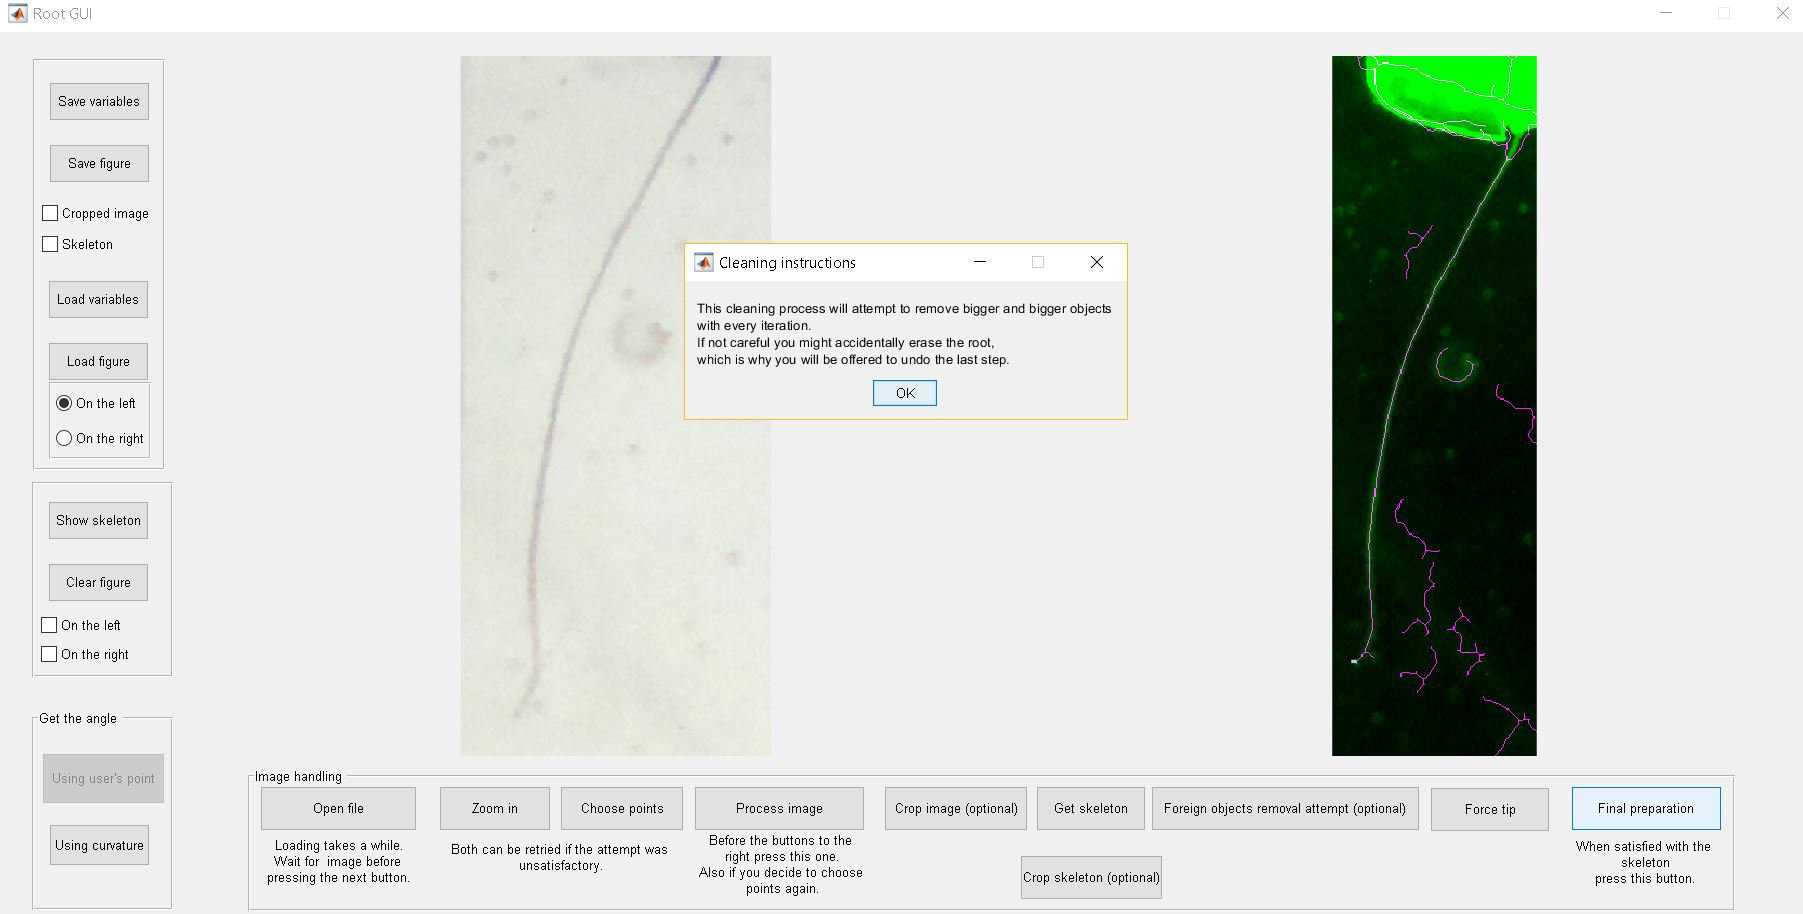
\includegraphics[width=\textwidth]{../Figures/manual/optionalA2.jpg}
	\caption{Explanation and instruction of the foreign objects removal step}
	\label{fig:img31}
\end{figure}

\begin{figure}[H]
	\centering
	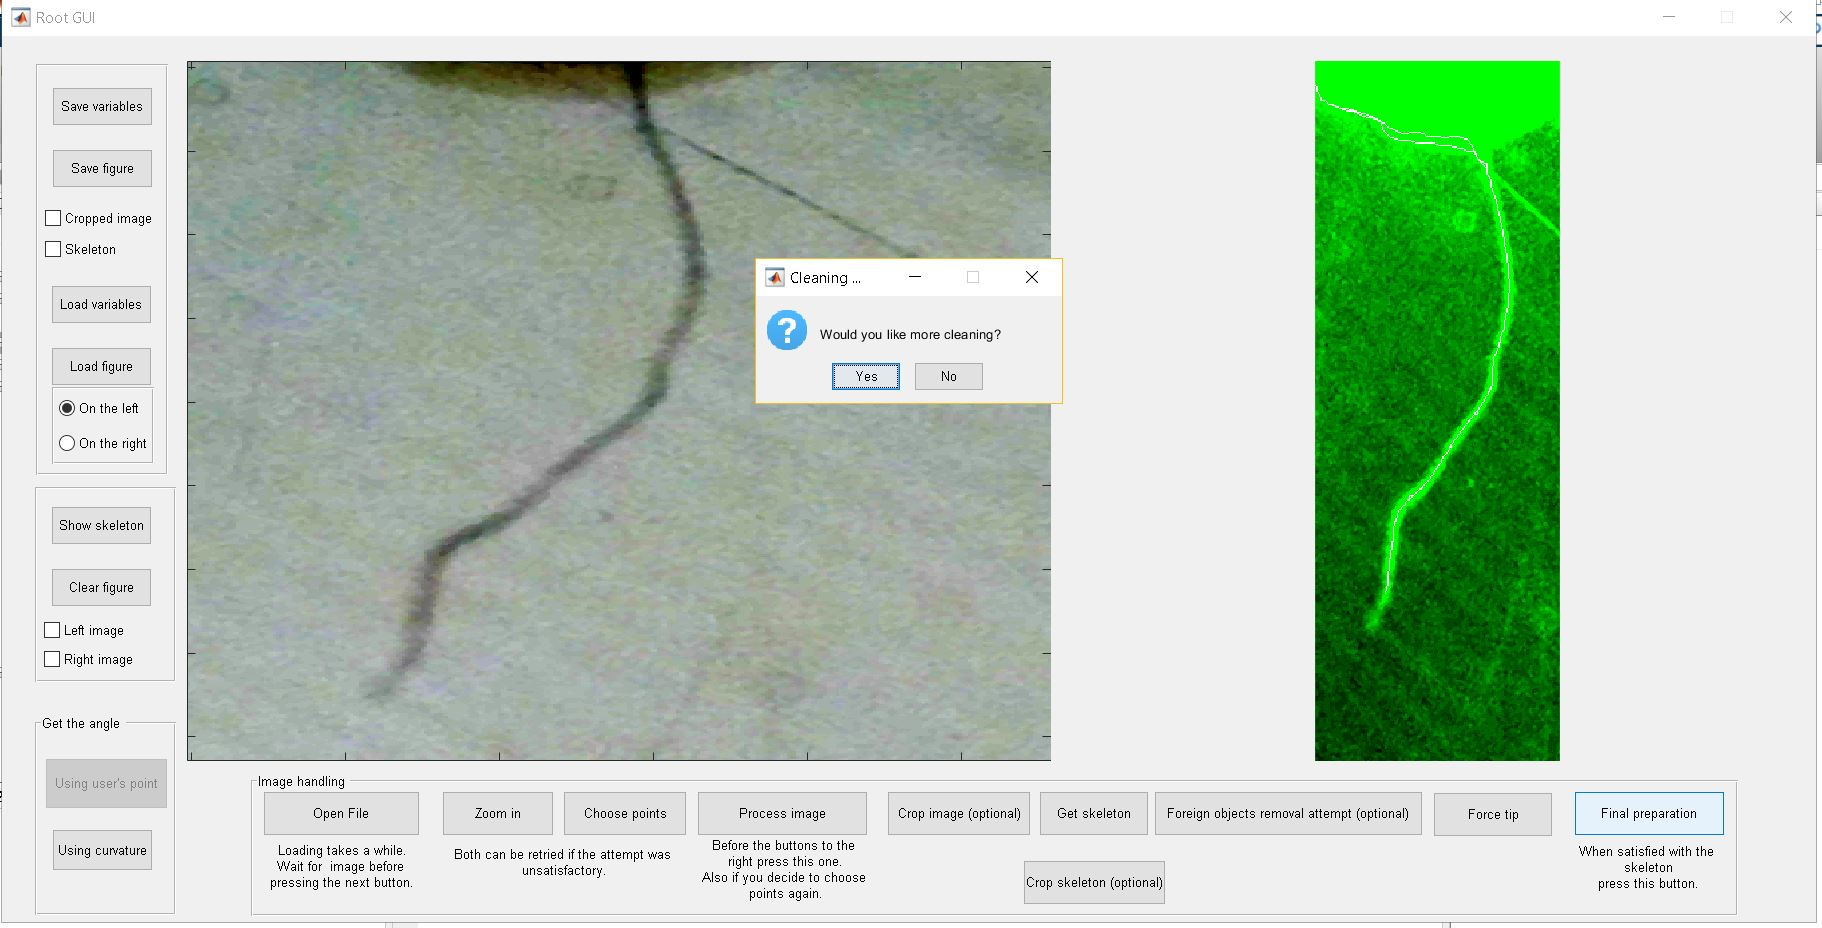
\includegraphics[width=\textwidth]{../Figures/manual/optionalA3.jpg}
	\caption{Prompt for further cleaning}
	\label{fig:img32}
\end{figure}

But what if you pressed 'Yes' once too often and the program deleted the skeleton, as it is in figure \ref{fig:img33}? 
Don't worry! There is an option to undo the last step. 
Just press 'No' and then you will be asked if you want to undo the last step (see figures \ref{fig:img34} -- \ref{fig:img35}).

\begin{figure}[H]
	\centering
	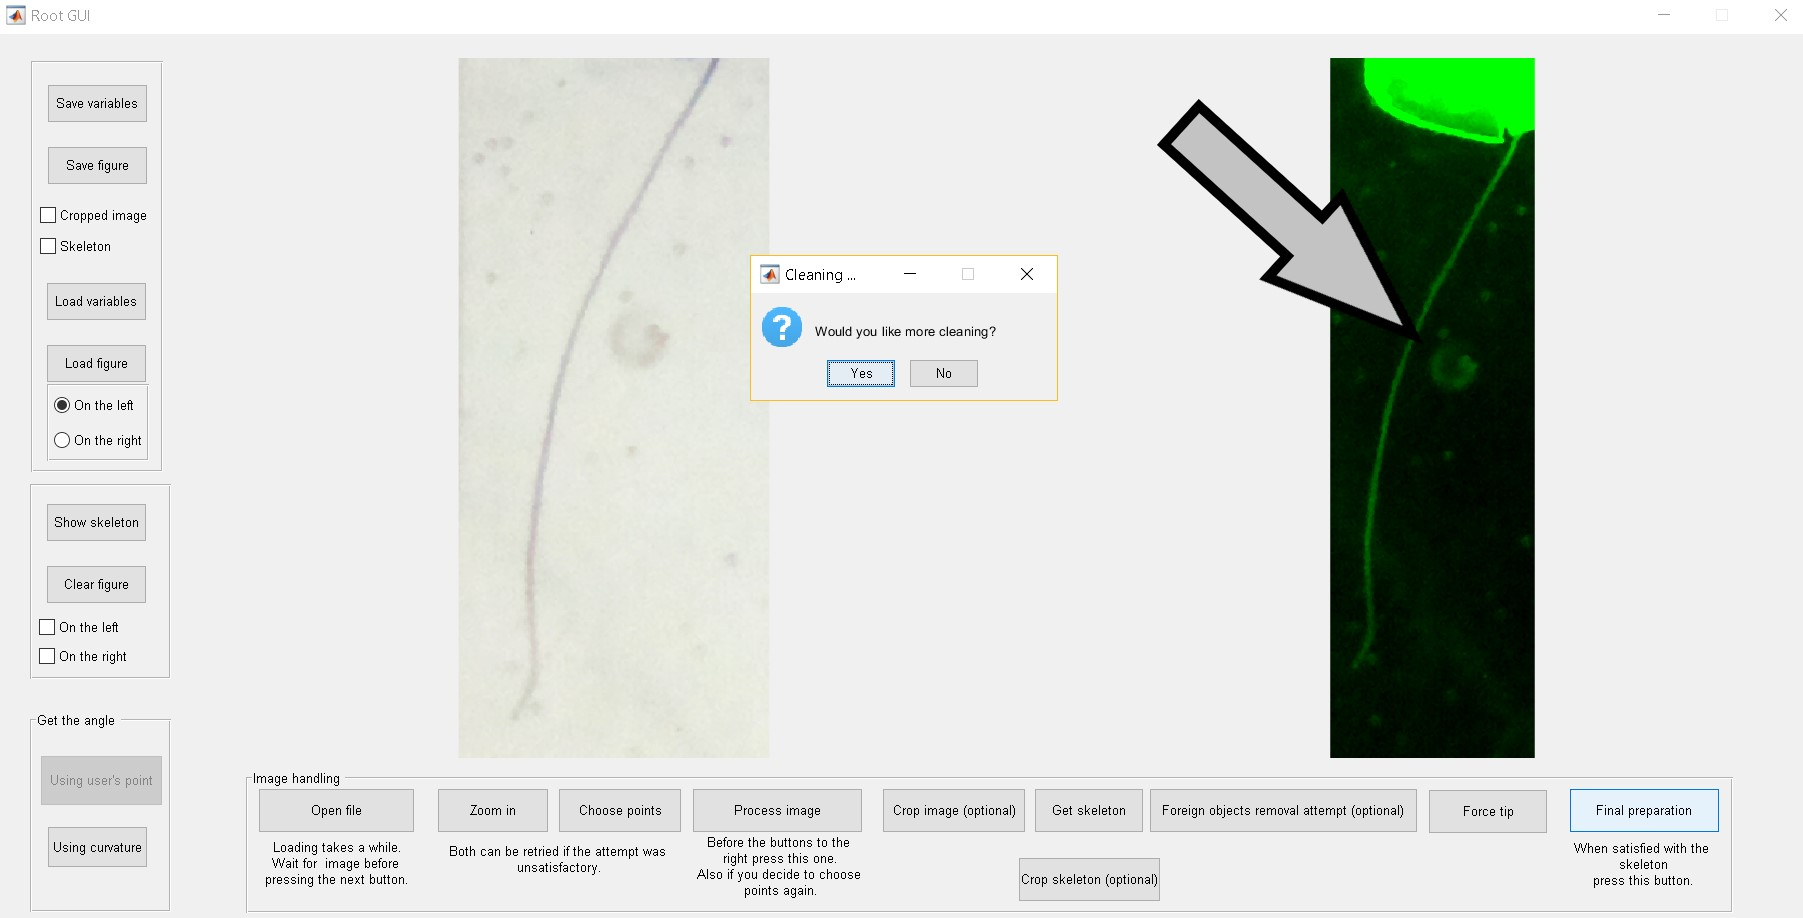
\includegraphics[width=\textwidth]{../Figures/manual/optionalA4.jpg}
	\caption{Prompt for futher cleaning when root is gone}
	\label{fig:img33}
\end{figure}

\begin{figure}[H]
	\centering
	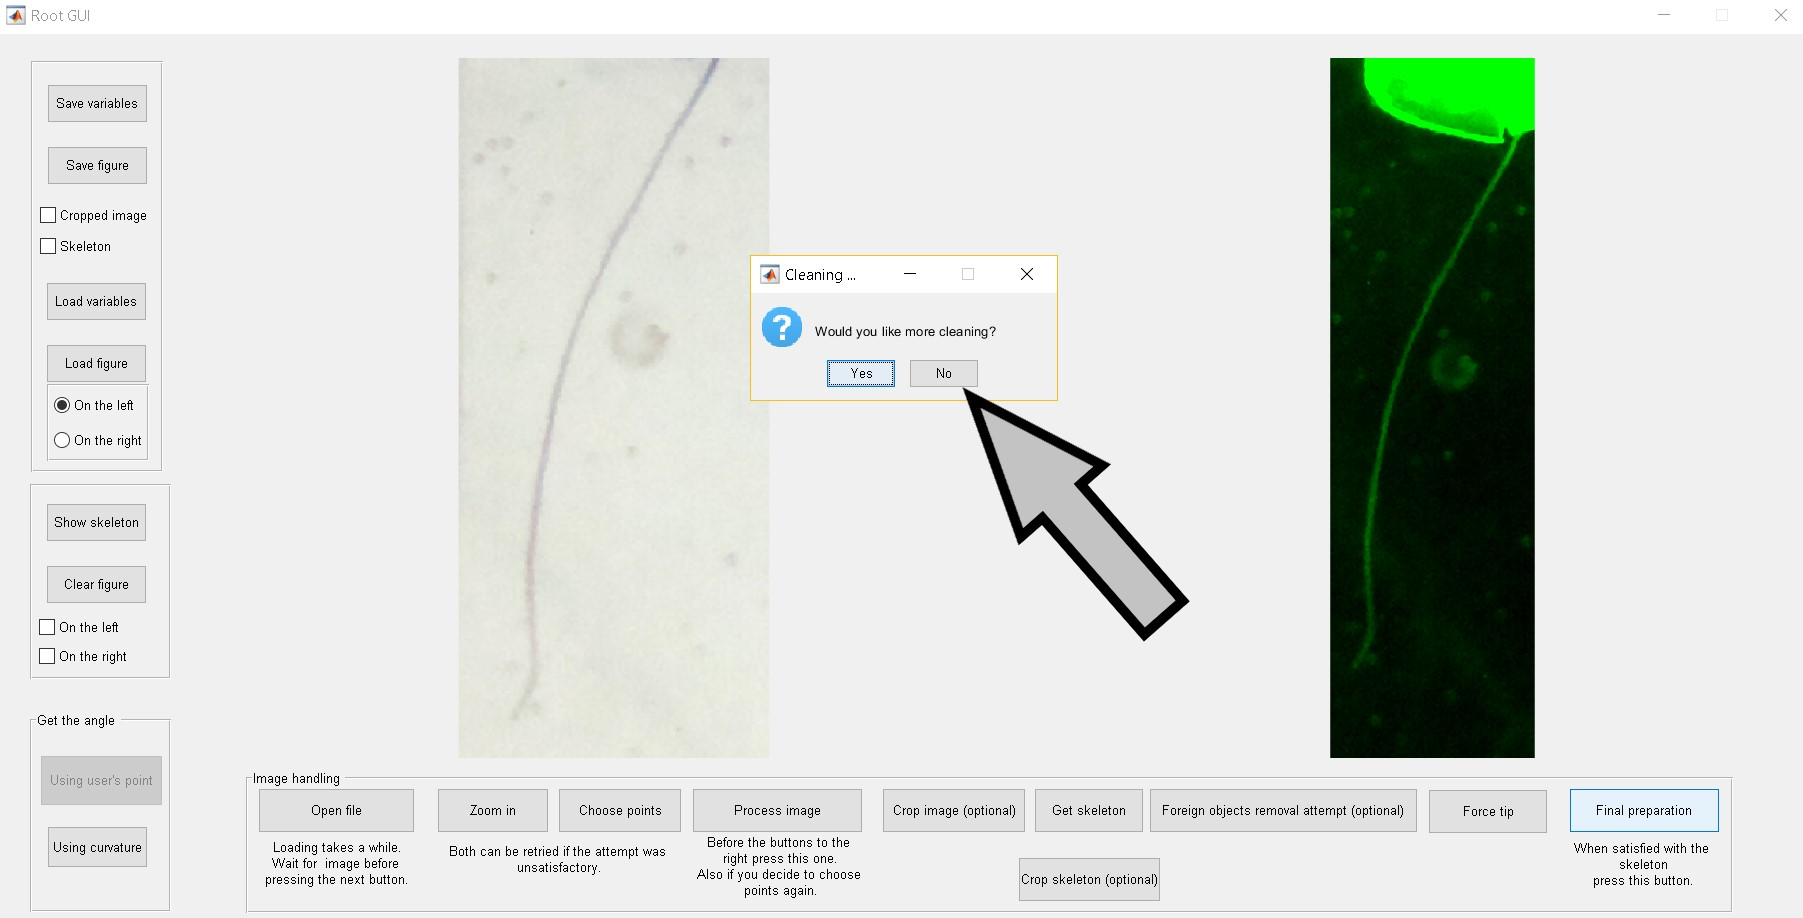
\includegraphics[width=\textwidth]{../Figures/manual/optionalA5.jpg}
	\caption{Clicking 'No' upon prompt for further cleaning}
	\label{fig:img34}
\end{figure}

\begin{figure}[H]
	\centering
	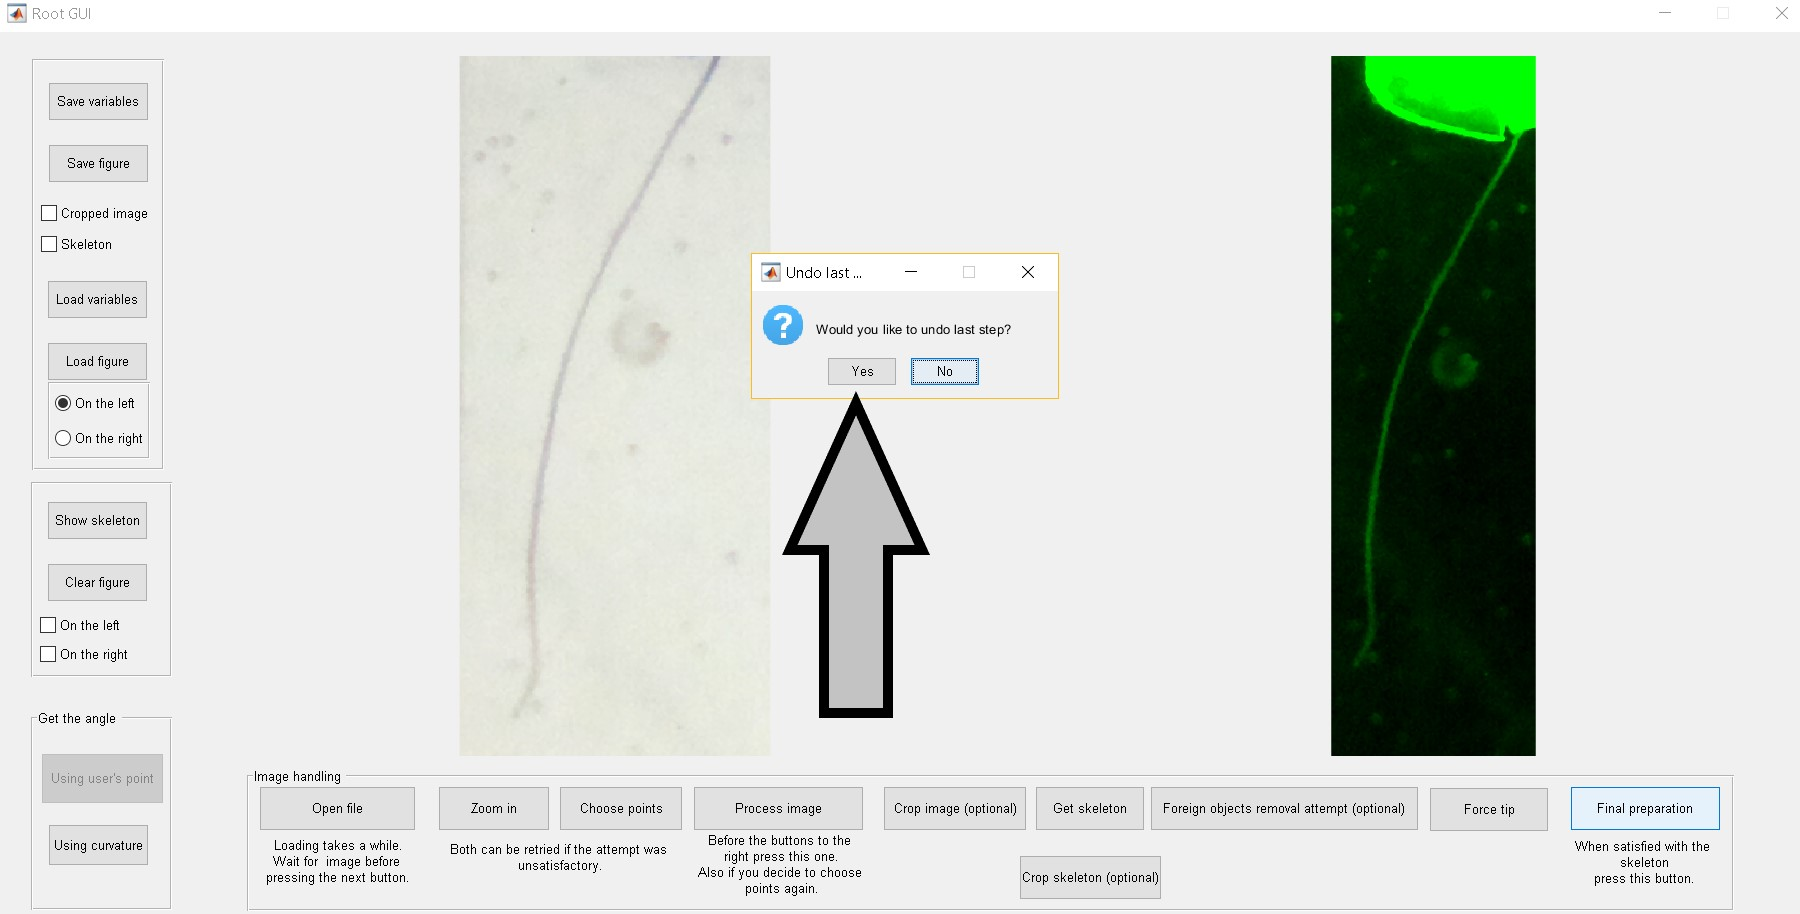
\includegraphics[width=\textwidth]{../Figures/manual/optionalA6.jpg}
	\caption{Clicking 'Yes' when asked to undo last step}
	\label{fig:img35}
\end{figure}

As you can see in figure \ref{fig:img36}, the skeleton "came back".

\begin{figure}[H]
	\centering
	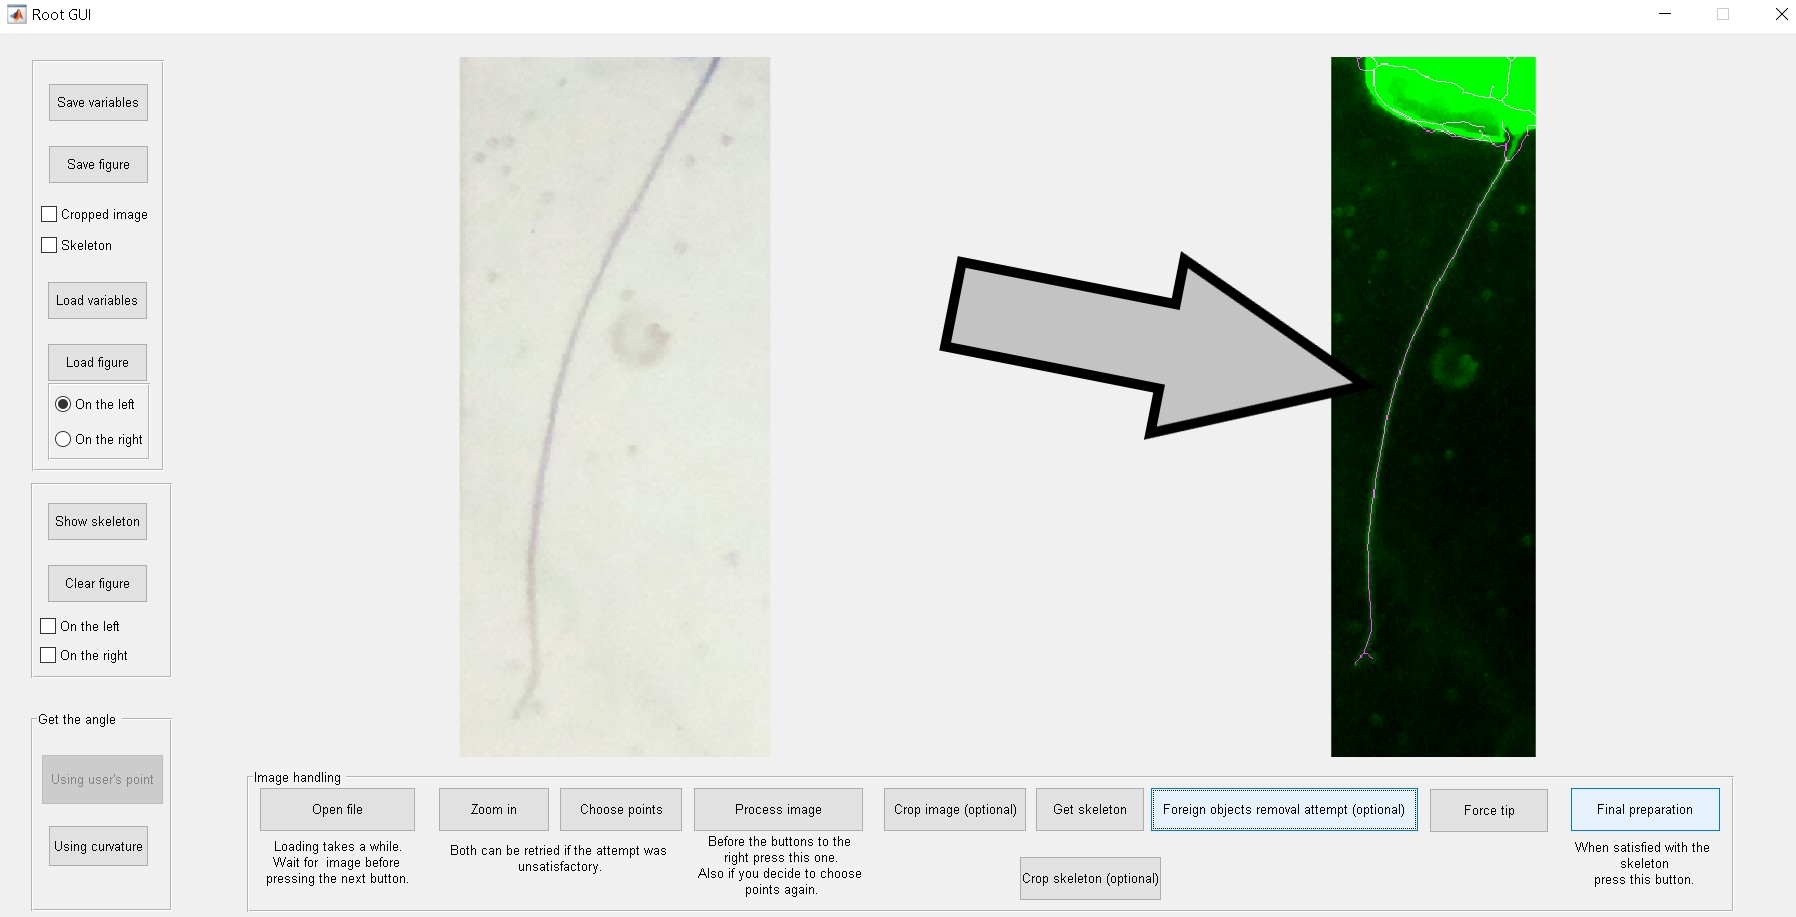
\includegraphics[width=\textwidth]{../Figures/manual/optionalA7.jpg}
	\caption{Upon undoing the last step the skeleton came back}
	\label{fig:img36}
\end{figure}


%----------------------------------------------------------------------------------------
\subsubsection{Force tip}

There are still various problems that can crop up but they can be solved.
For example, what if the skeleton you got doesnt't get all the way to the tip of the root? 
Well, that's a task for \textit{Force tip}, that enforces the tip of the root to be contained in the skeleton. 
So first you click the button \textit{Force tip} (see figure \ref{fig:img37}), then a message pops up asking you to drag a line from the end of the skeleton to the tip (see figure \ref{fig:img38}).
But we can actually do it in more than one step. For example, in the example given here it seems like a straight line from the skeleton to the tip won't follow the root. 
So let's first do the short line on figure \ref{fig:img39}, then to see how it looks, we can click on \textit{Show skeleton} (see figures \ref{fig:img40} -- \ref{fig:img41}),
and we'll see the skeleton alone on the left and overlaid on the root on the right. 
And then, we'll draw the final line (see figure \ref{fig:img42}).
We'll click on \textit{Show skeleton} again to see if we are pleased (see figure \ref{fig:img43}), then on \textit{Final preparation} and we'll see that we get a reasonable angle (see figures \ref{fig:img44} -- \ref{fig:img45}).


\begin{figure}[H]
	\centering
	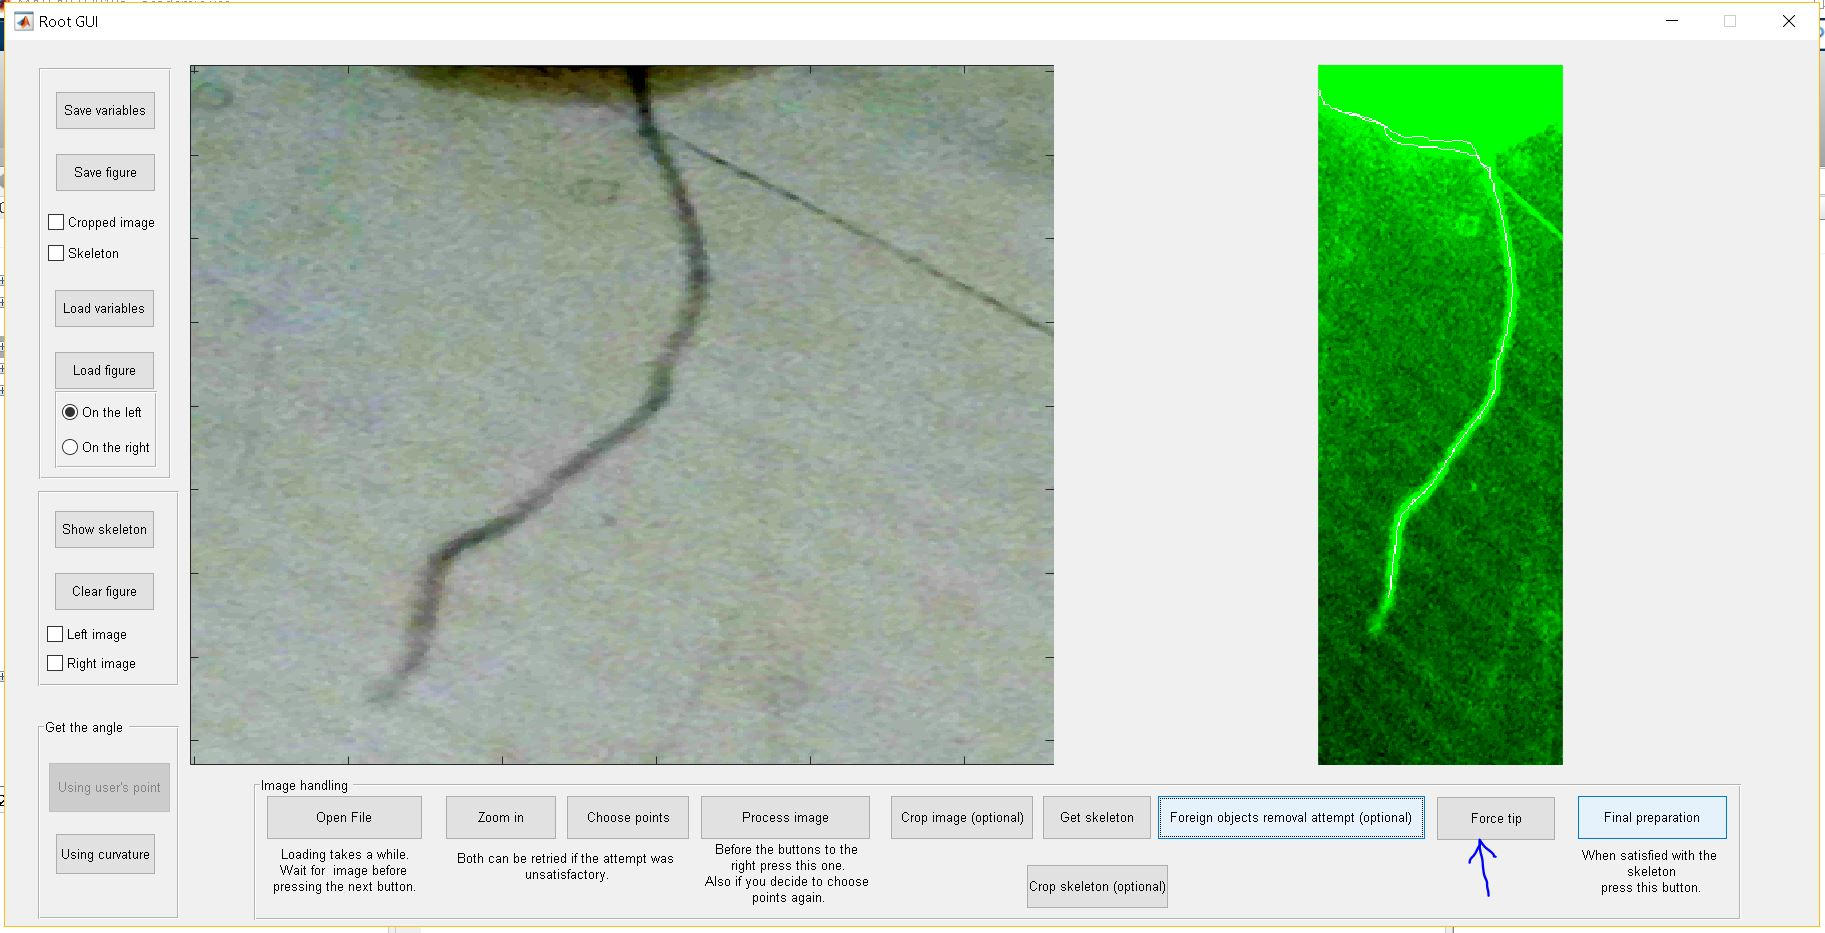
\includegraphics[width=\textwidth]{../Figures/manual/optionalB1.jpg}
	\caption{Optional step in the \textit{RootSkel} pipeline: Force tip}
	\label{fig:img37}
\end{figure}

\begin{figure}[H]
	\centering
	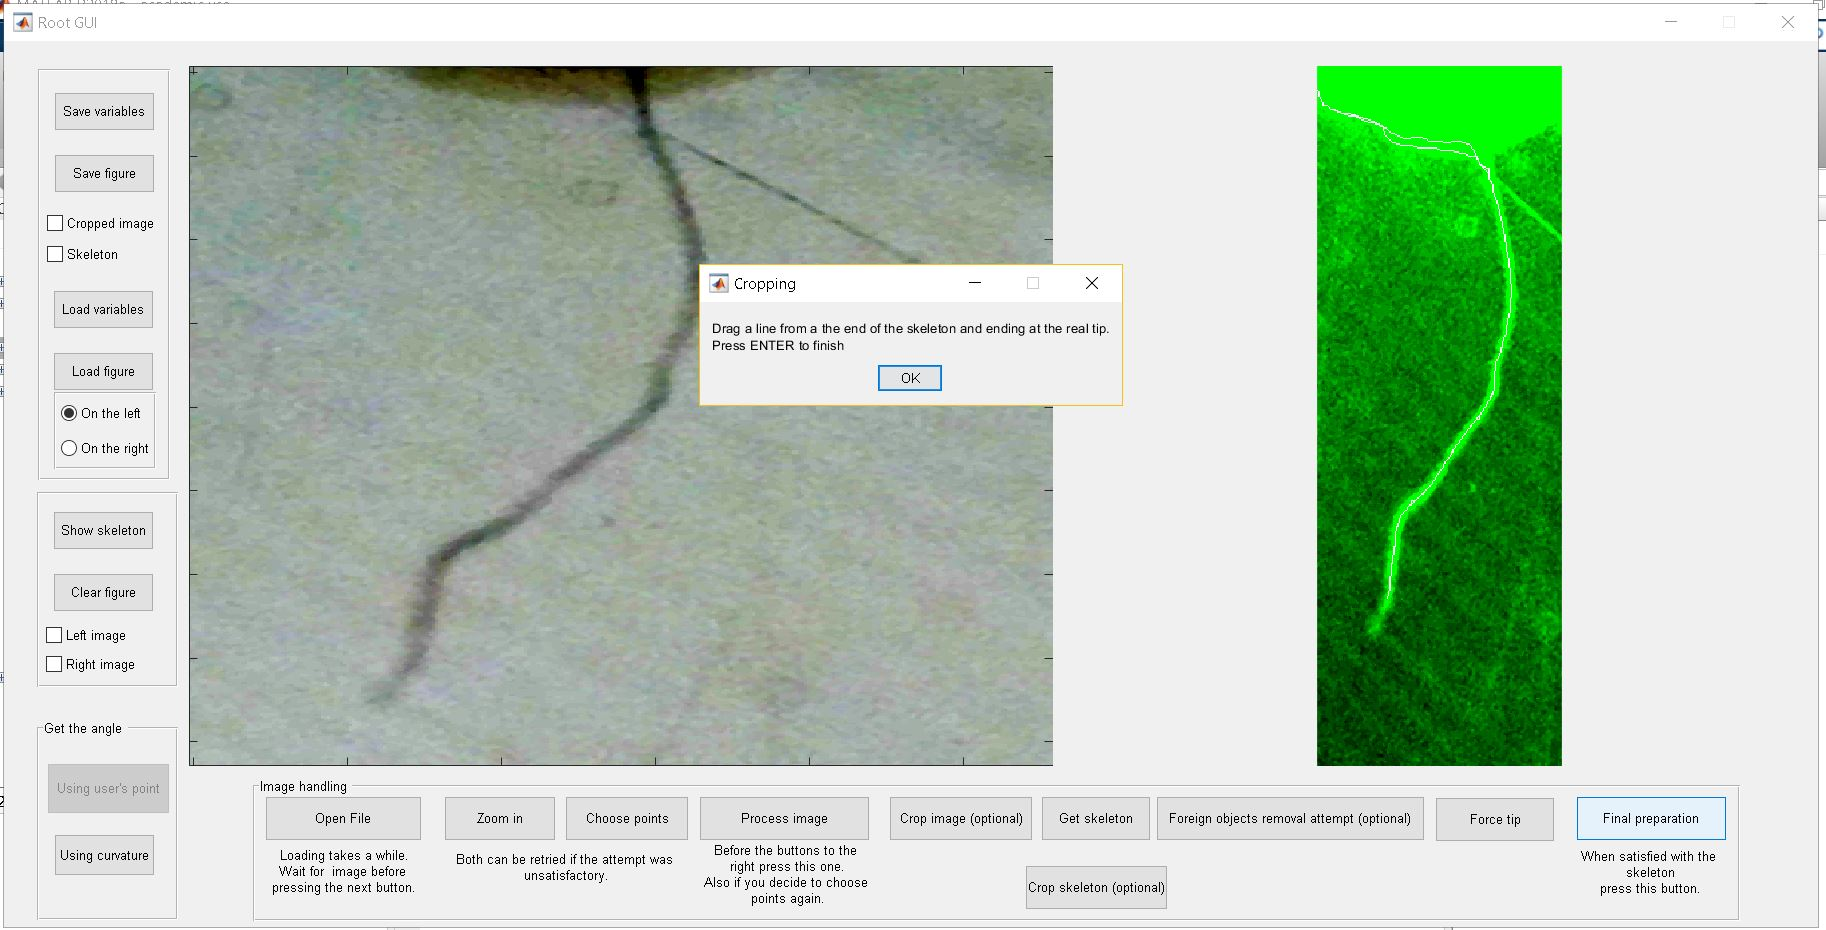
\includegraphics[width=\textwidth]{../Figures/manual/optionalB2.jpg}
	\caption{Instructions upon clicking on \textit{Force tip}}
	\label{fig:img38}
\end{figure}

\begin{figure}[H]
	\centering
	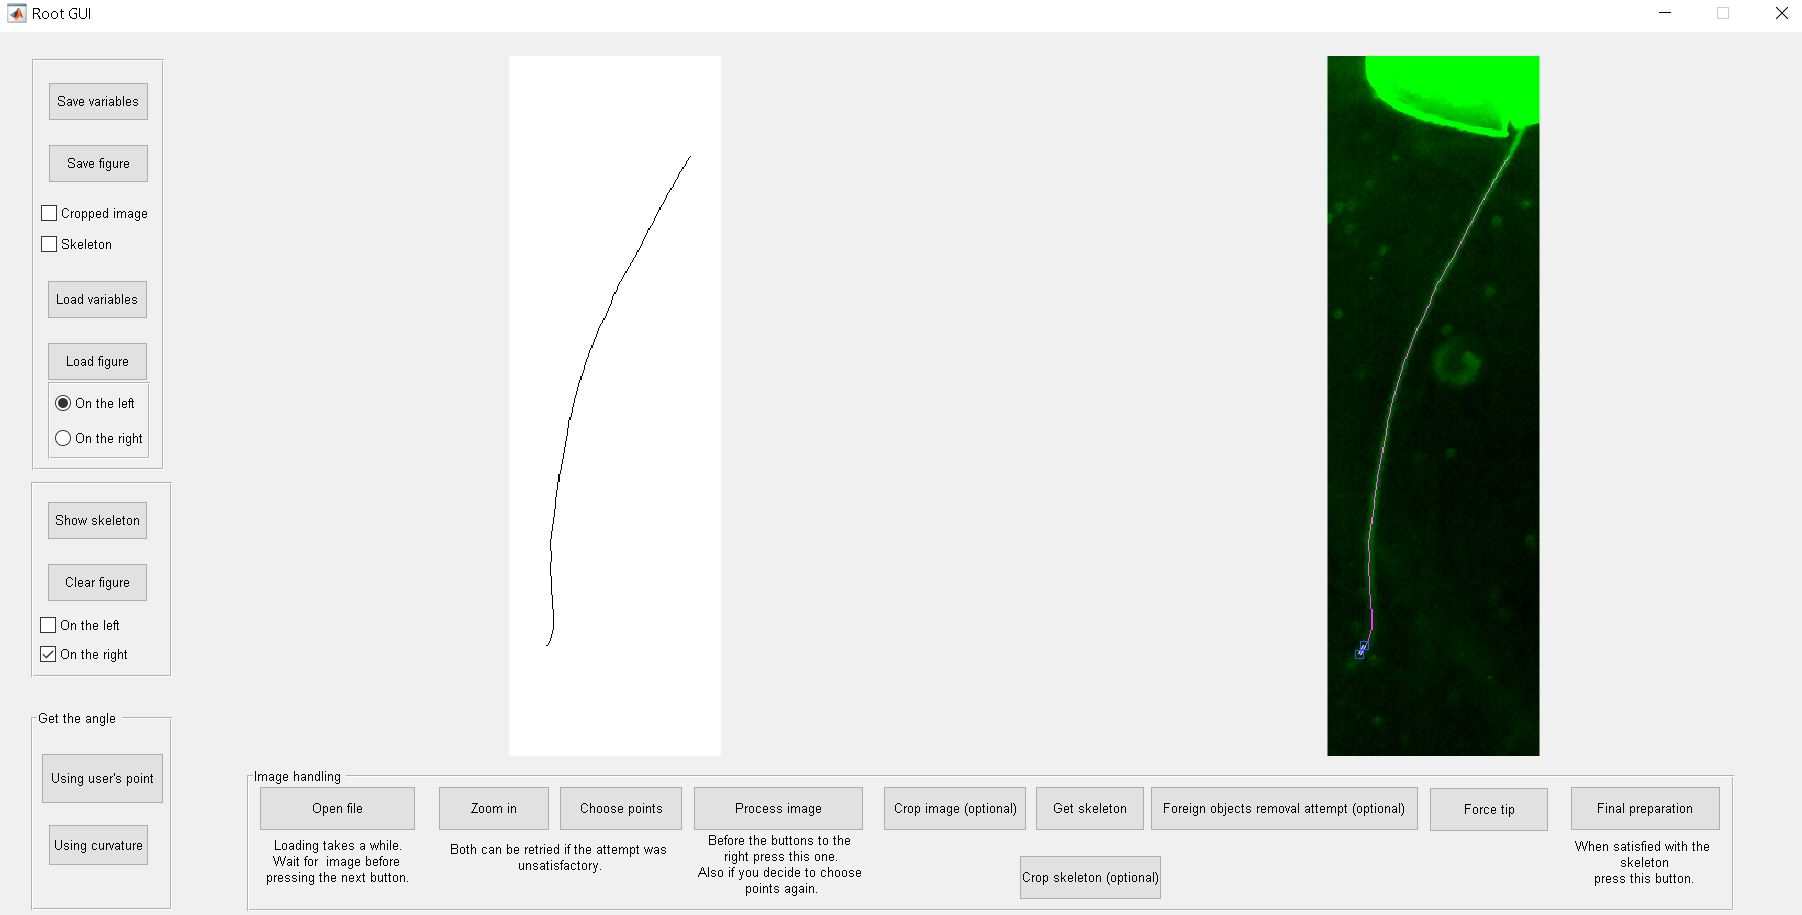
\includegraphics[width=\textwidth]{../Figures/manual/optionalB3.jpg}
%	\caption{Applying \textit{force tip}: Elongating the tip of the root skeleton}
	\caption{Applying \textit{force tip}: Trying to elongate the tip of the root with a line}
	\label{fig:img39}
\end{figure}

\begin{figure}[H]
	\centering
	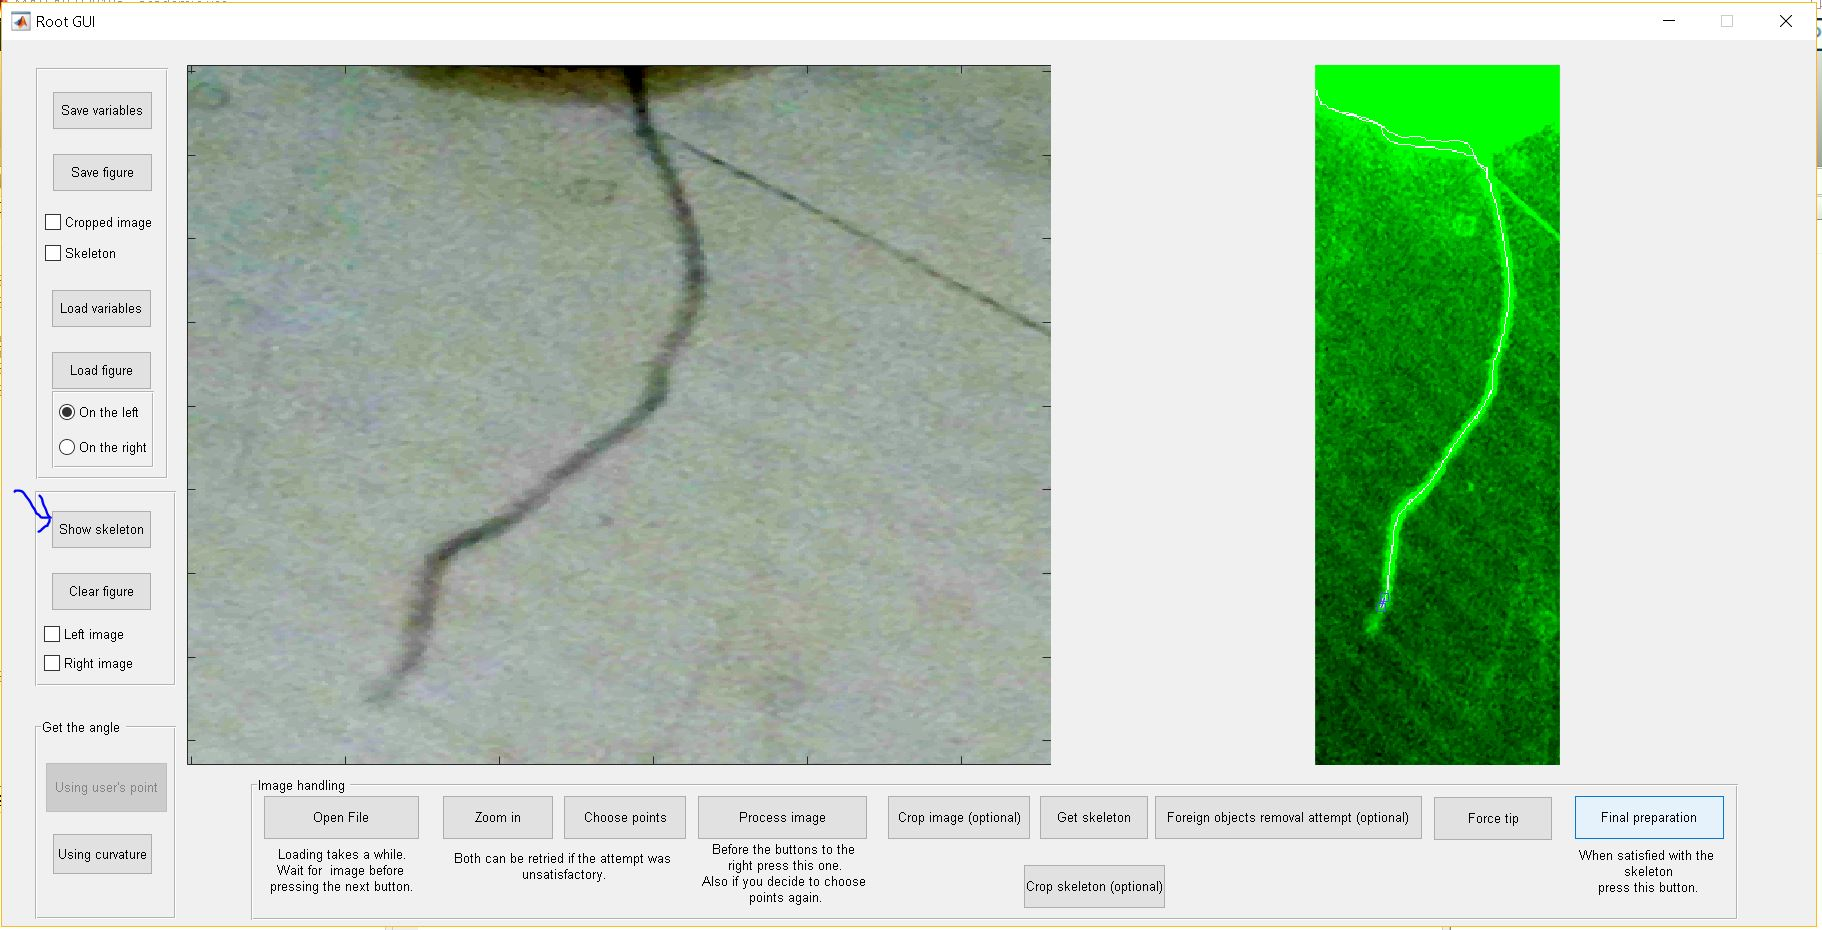
\includegraphics[width=\textwidth]{../Figures/manual/optionalB4.jpg}
	\caption{Clicking on \textit{Show skeleton} to show the new skeleton}
	\label{fig:img40}
\end{figure}

\begin{figure}[H]
	\centering
	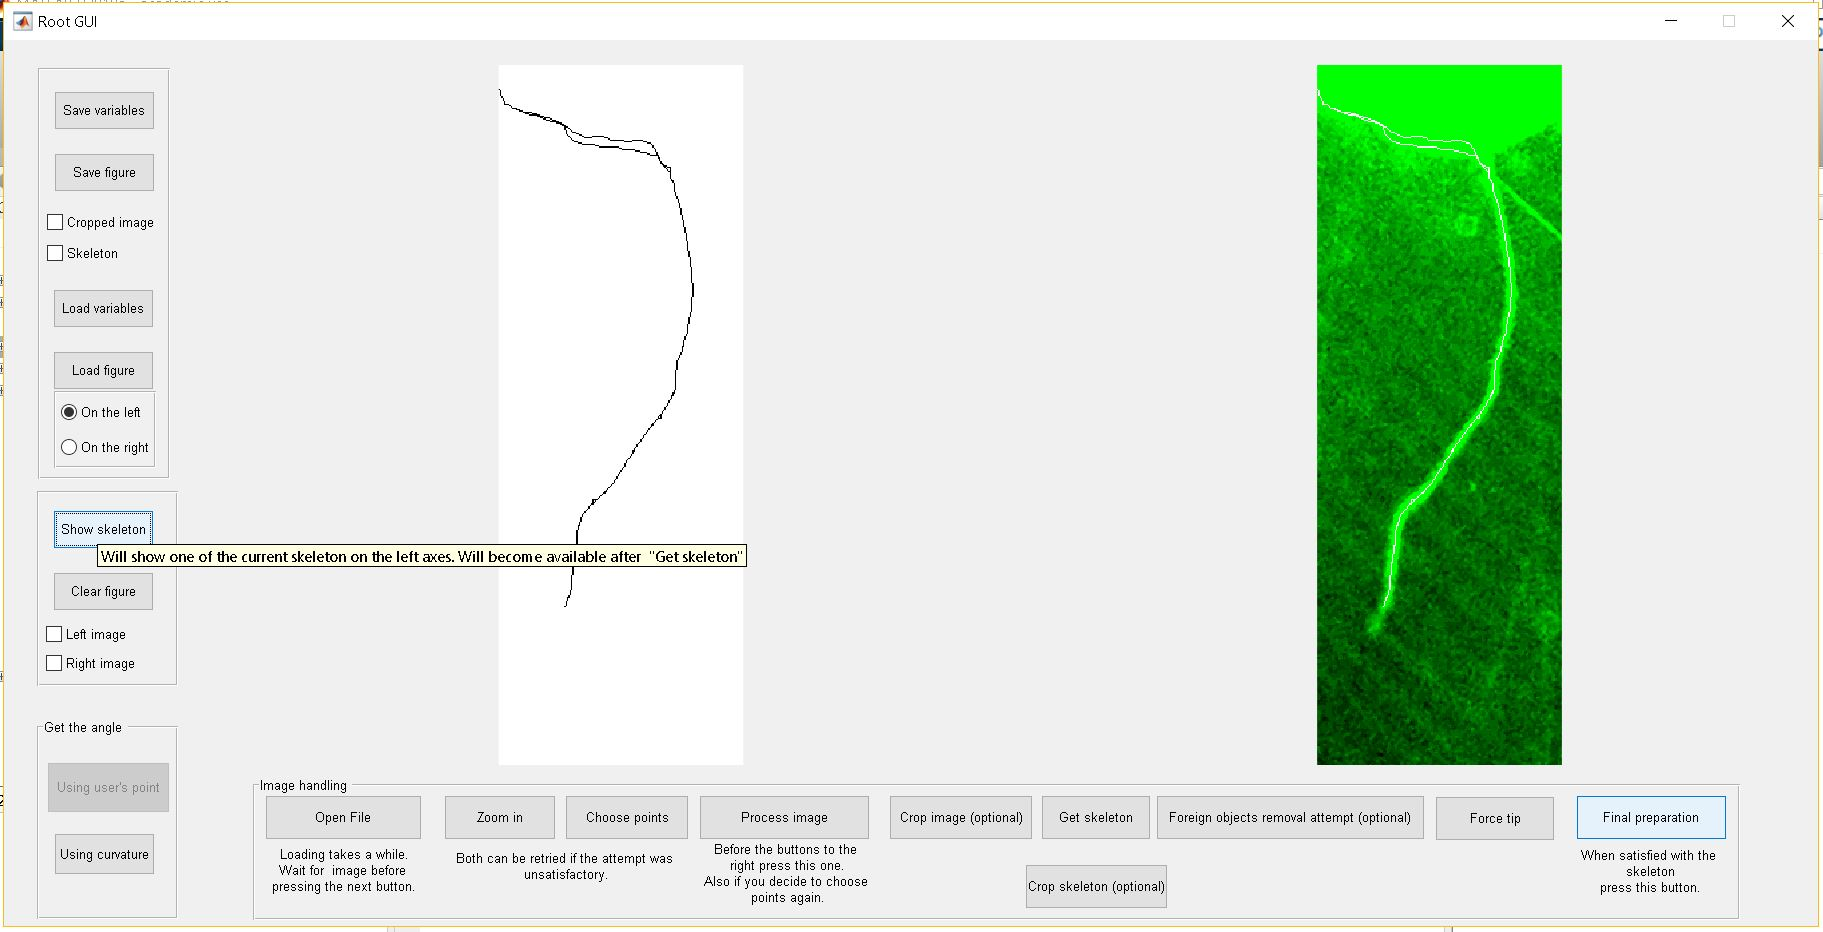
\includegraphics[width=\textwidth]{../Figures/manual/optionalB5.jpg}
	\caption{Message upon hovering over the \textit{Show skeleton} button}
	\label{fig:img41}
\end{figure}

\begin{figure}[H]
	\centering
	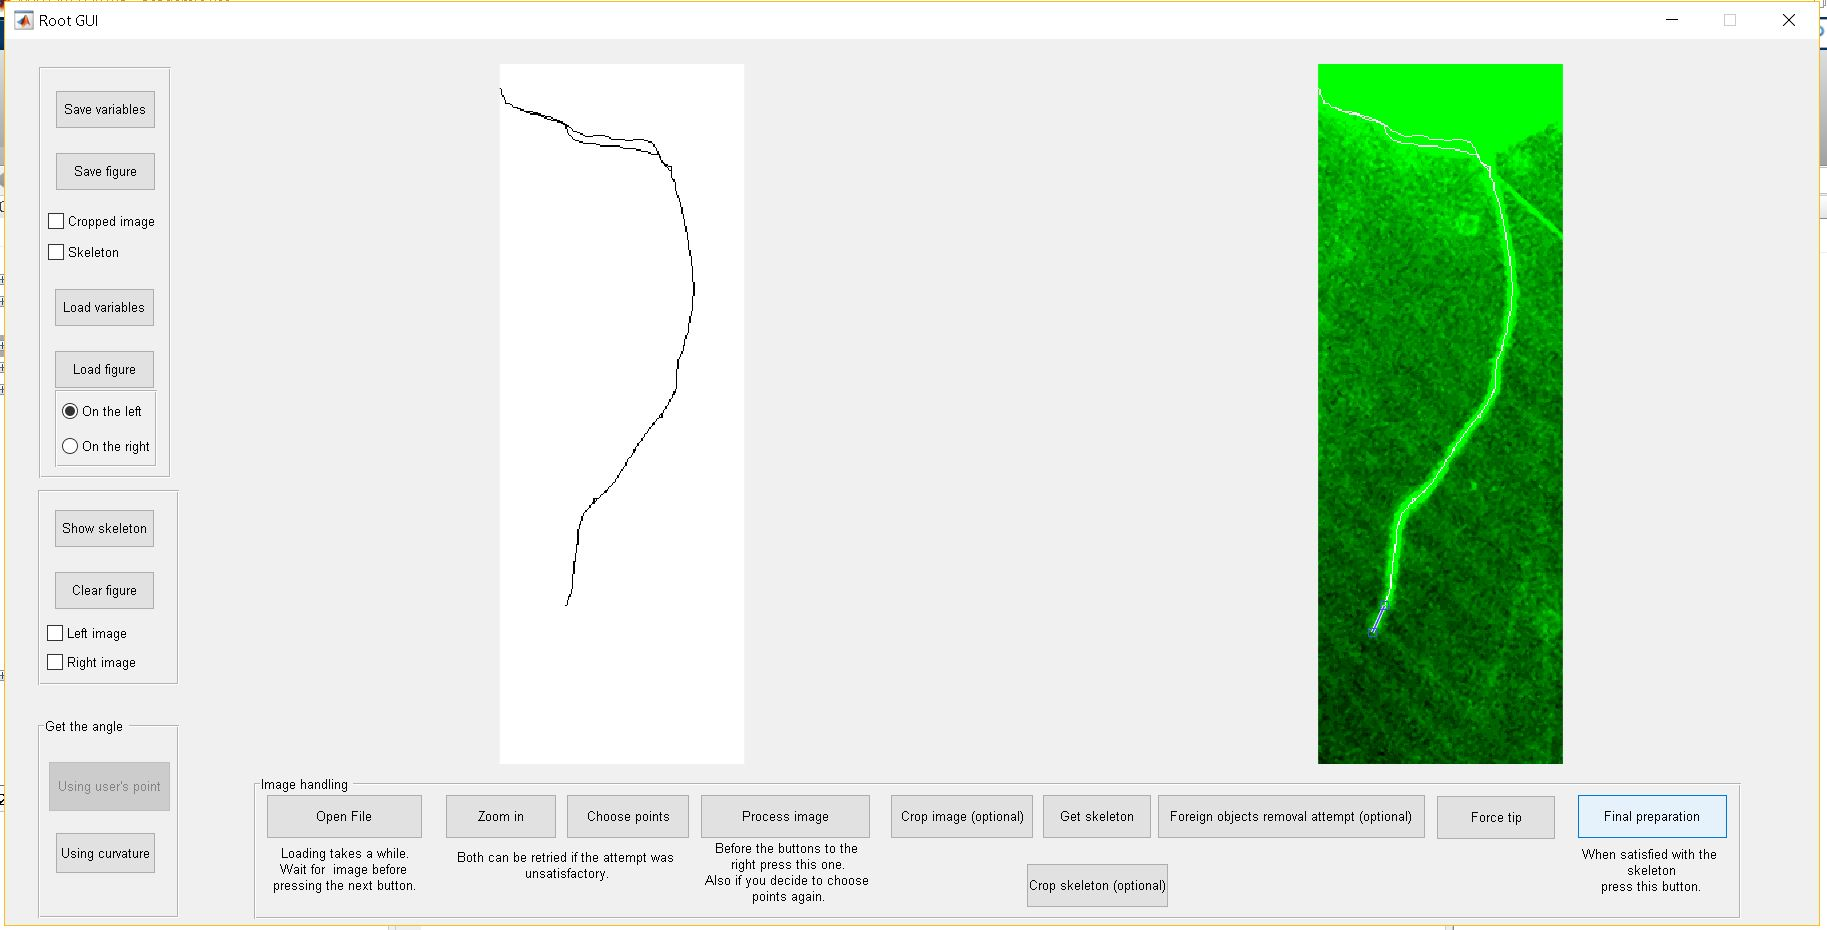
\includegraphics[width=\textwidth]{../Figures/manual/optionalB6.jpg}
	\caption{The current skeleton}
	\label{fig:img42}
\end{figure}

\begin{figure}[H]
	\centering
	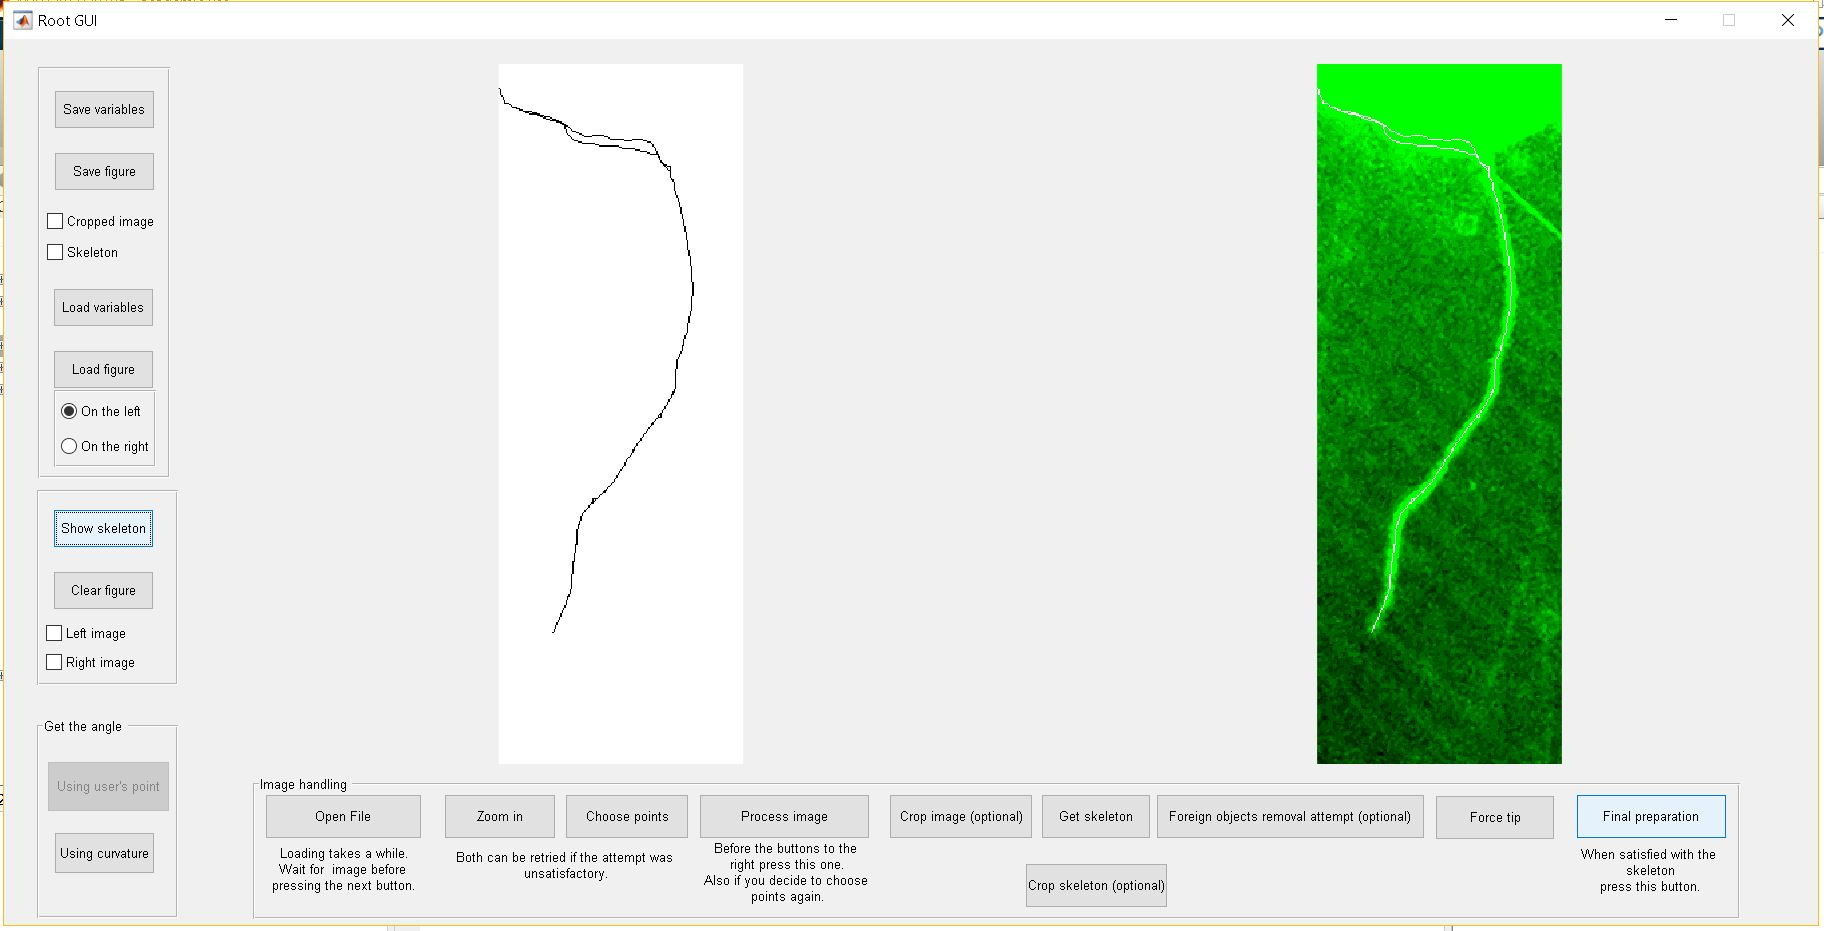
\includegraphics[width=\textwidth]{../Figures/manual/optionalB7.jpg}
%    \caption{Applying \textit{force tip}: Trying to elongate the tip of the root with a line}
	\caption{Upon clicking \textit{Show skeleton}: The elongated tip skeleton}
	\label{fig:img43}
\end{figure}

\begin{figure}[H]
	\centering
	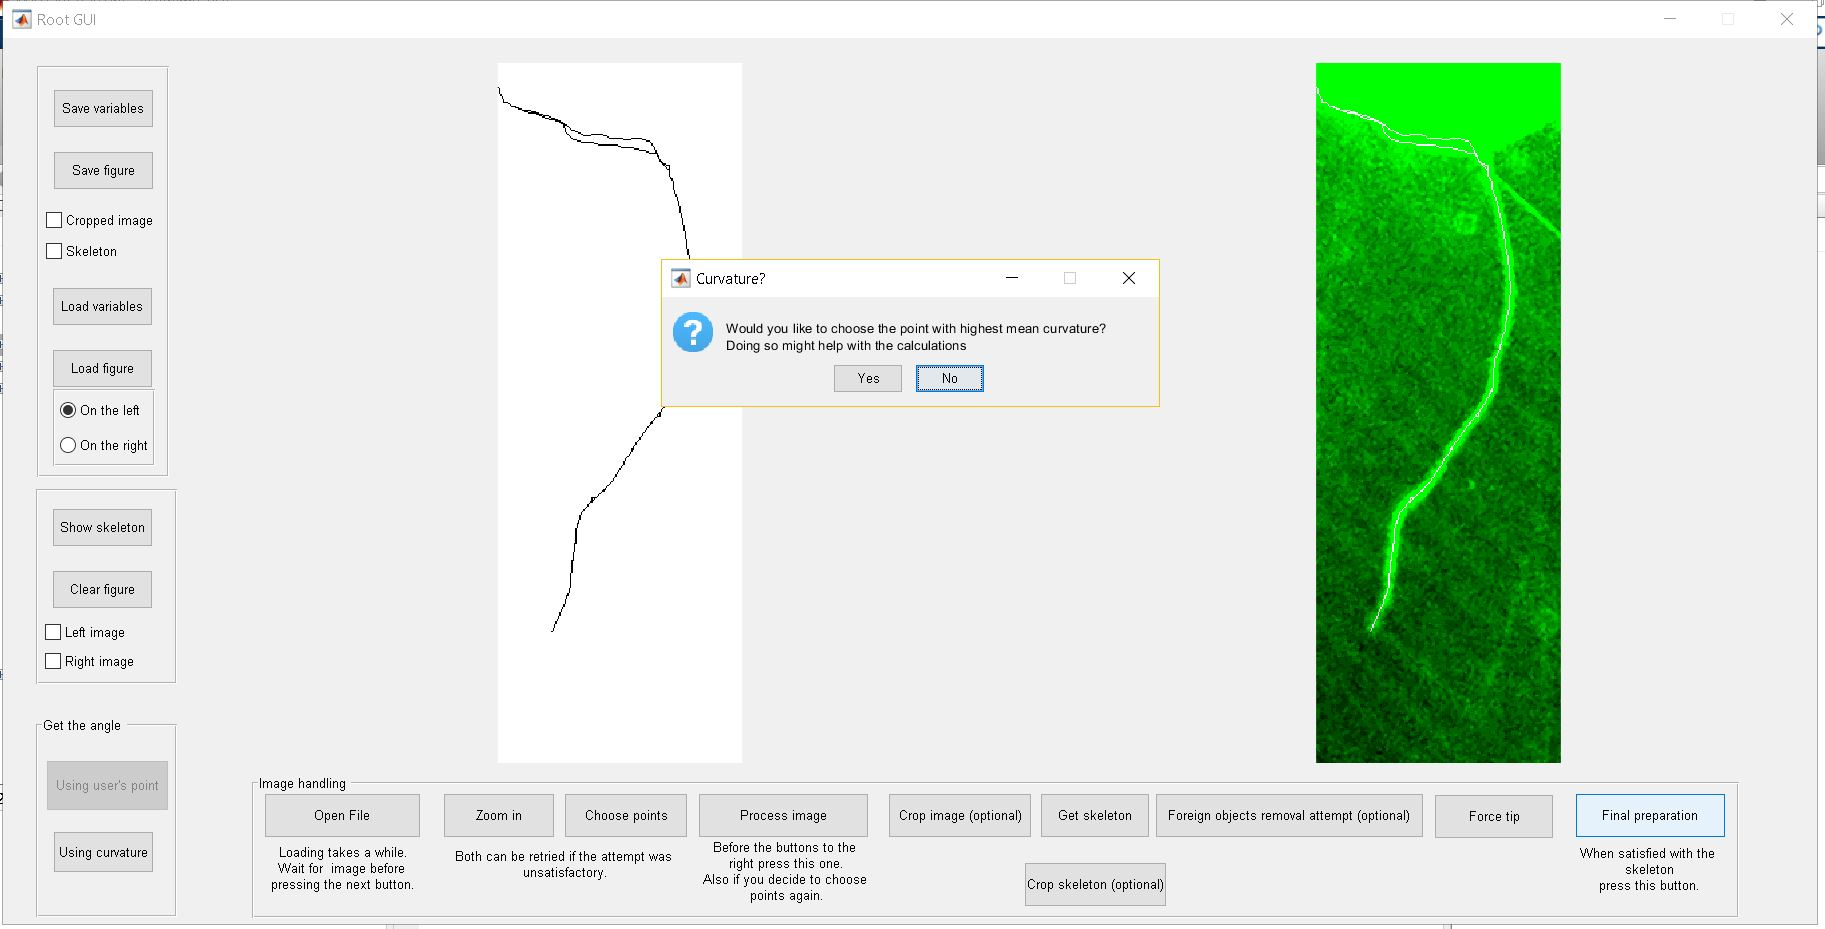
\includegraphics[width=\textwidth]{../Figures/manual/optionalB8.jpg}
	\caption{Clicking 'No' when asked to optionally choose a point of highest local (mean) curvature}
	\label{fig:img44}
\end{figure}

\begin{figure}[H]
	\centering
	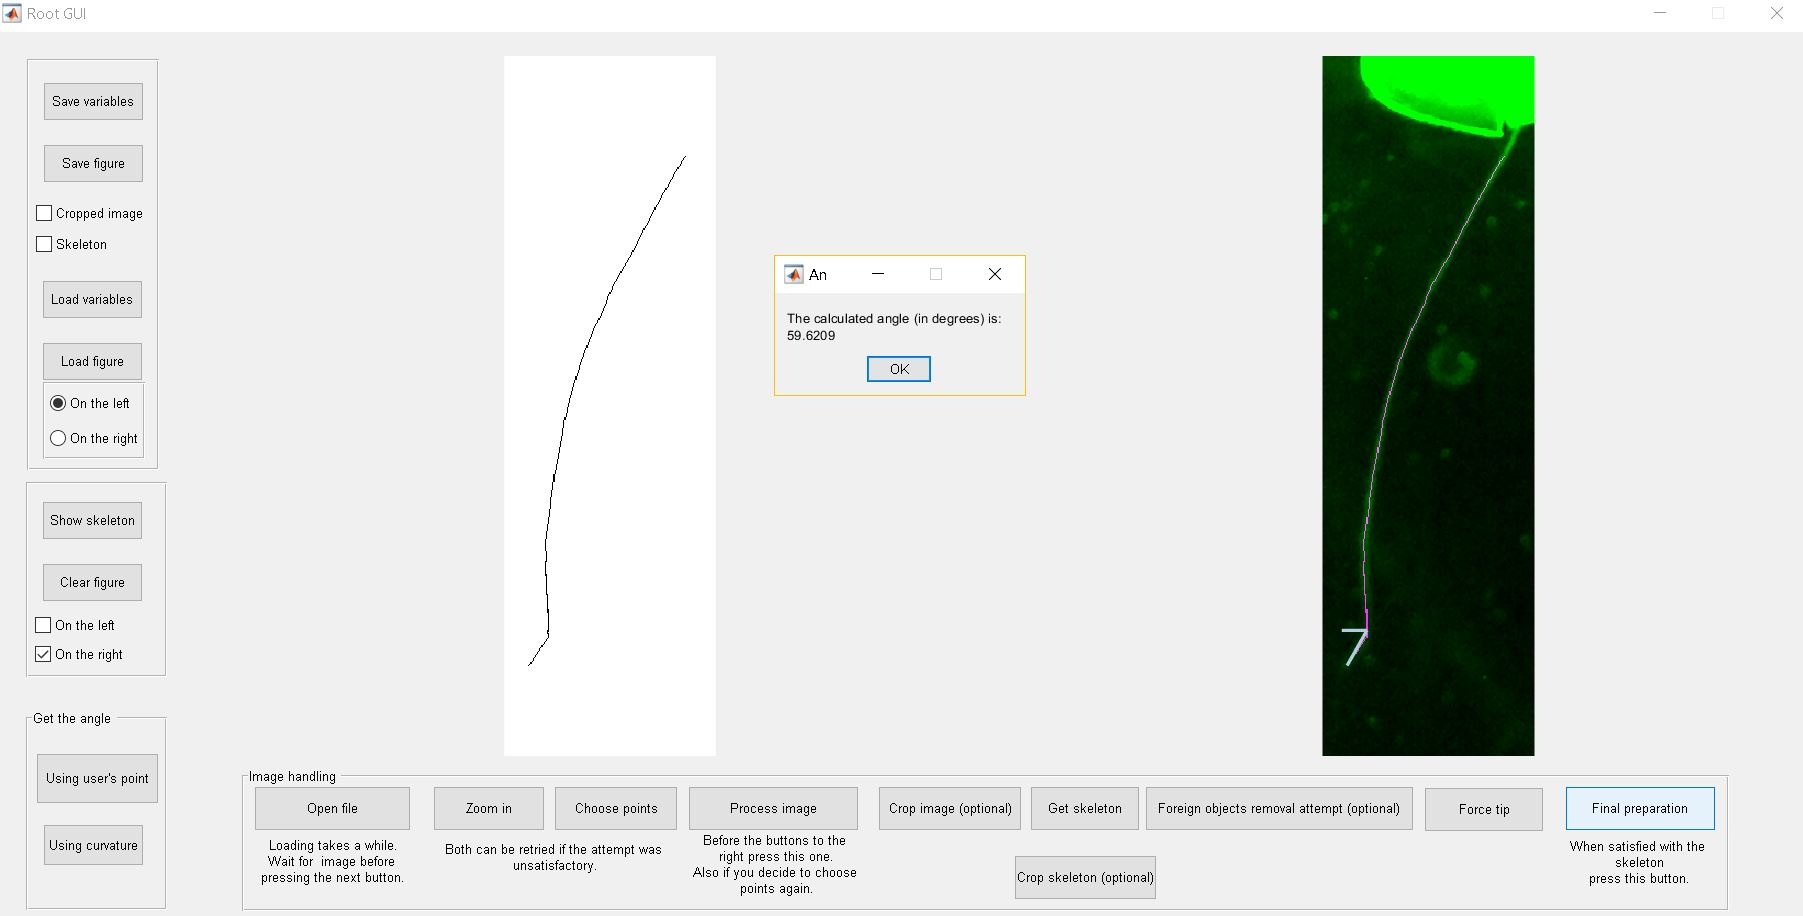
\includegraphics[width=\textwidth]{../Figures/manual/optionalB9.jpg}
	\caption{The calculated angle in a pop up window}
	\label{fig:img45}
\end{figure}


%----------------------------------------------------------------------------------------
\subsubsection{Crop image}

Let's say we have a problem like the one in figure \ref{fig:img46}.

\begin{figure}[H]
	\centering
	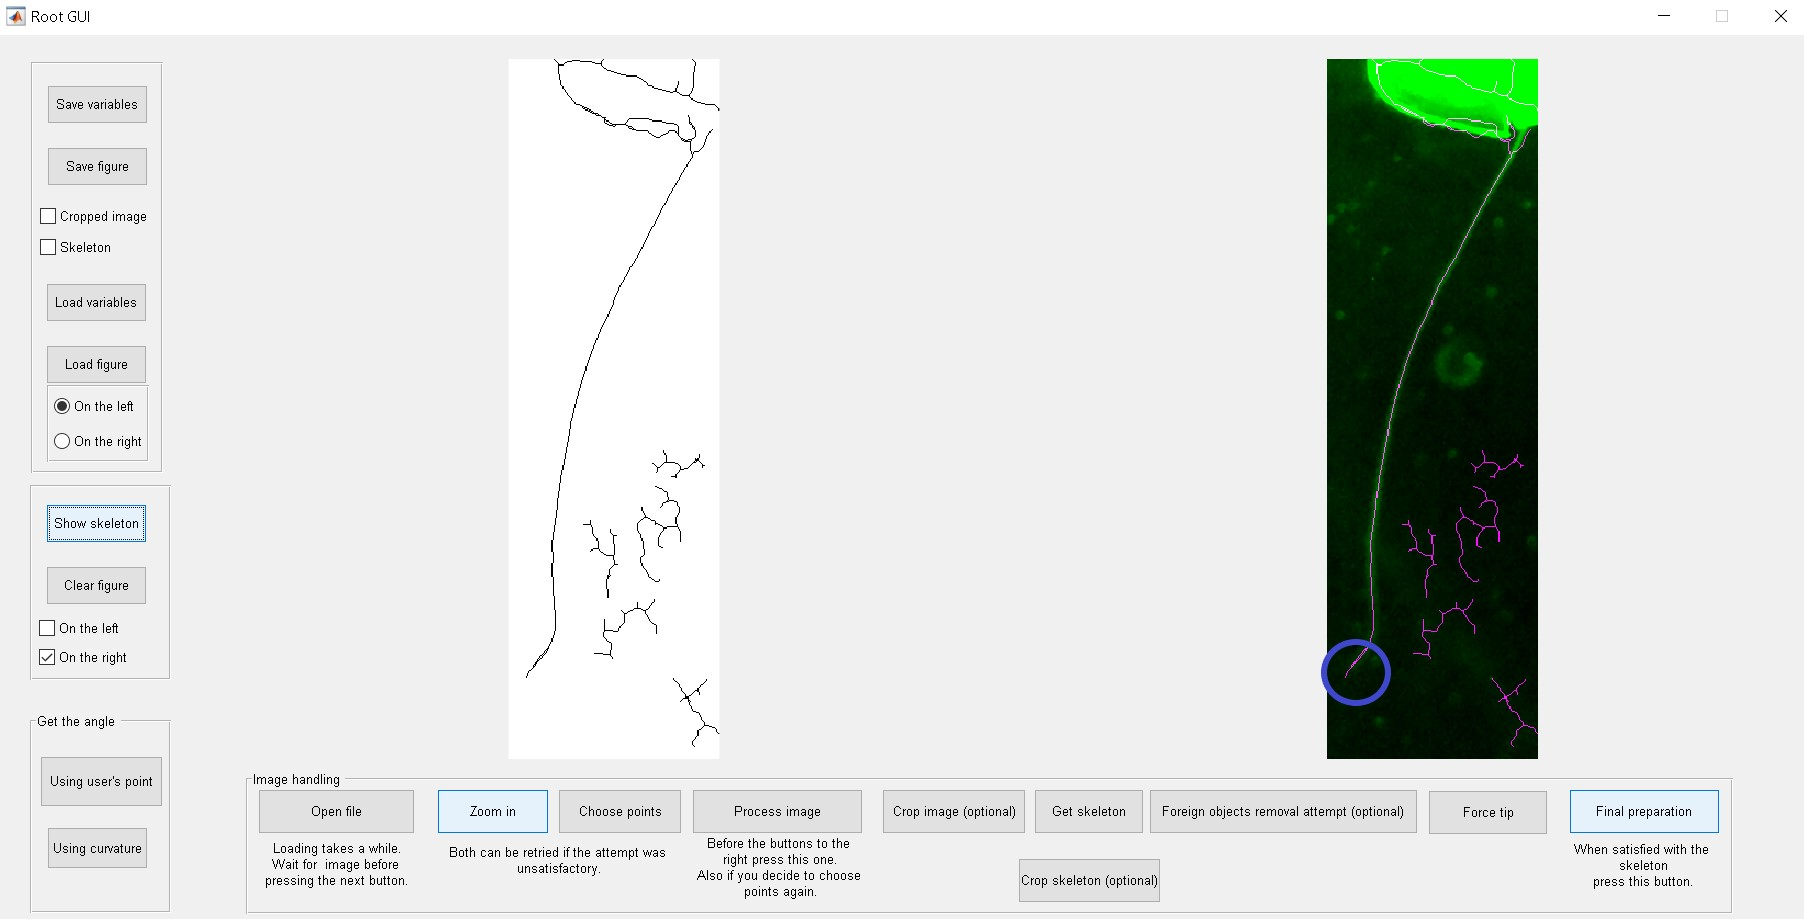
\includegraphics[width=\textwidth]{../Figures/manual/optionalC1.jpg}
	\caption{Unwanted branches in the root skeleton}
	\label{fig:img46}
\end{figure}

\begin{figure}[H]
	\centering
	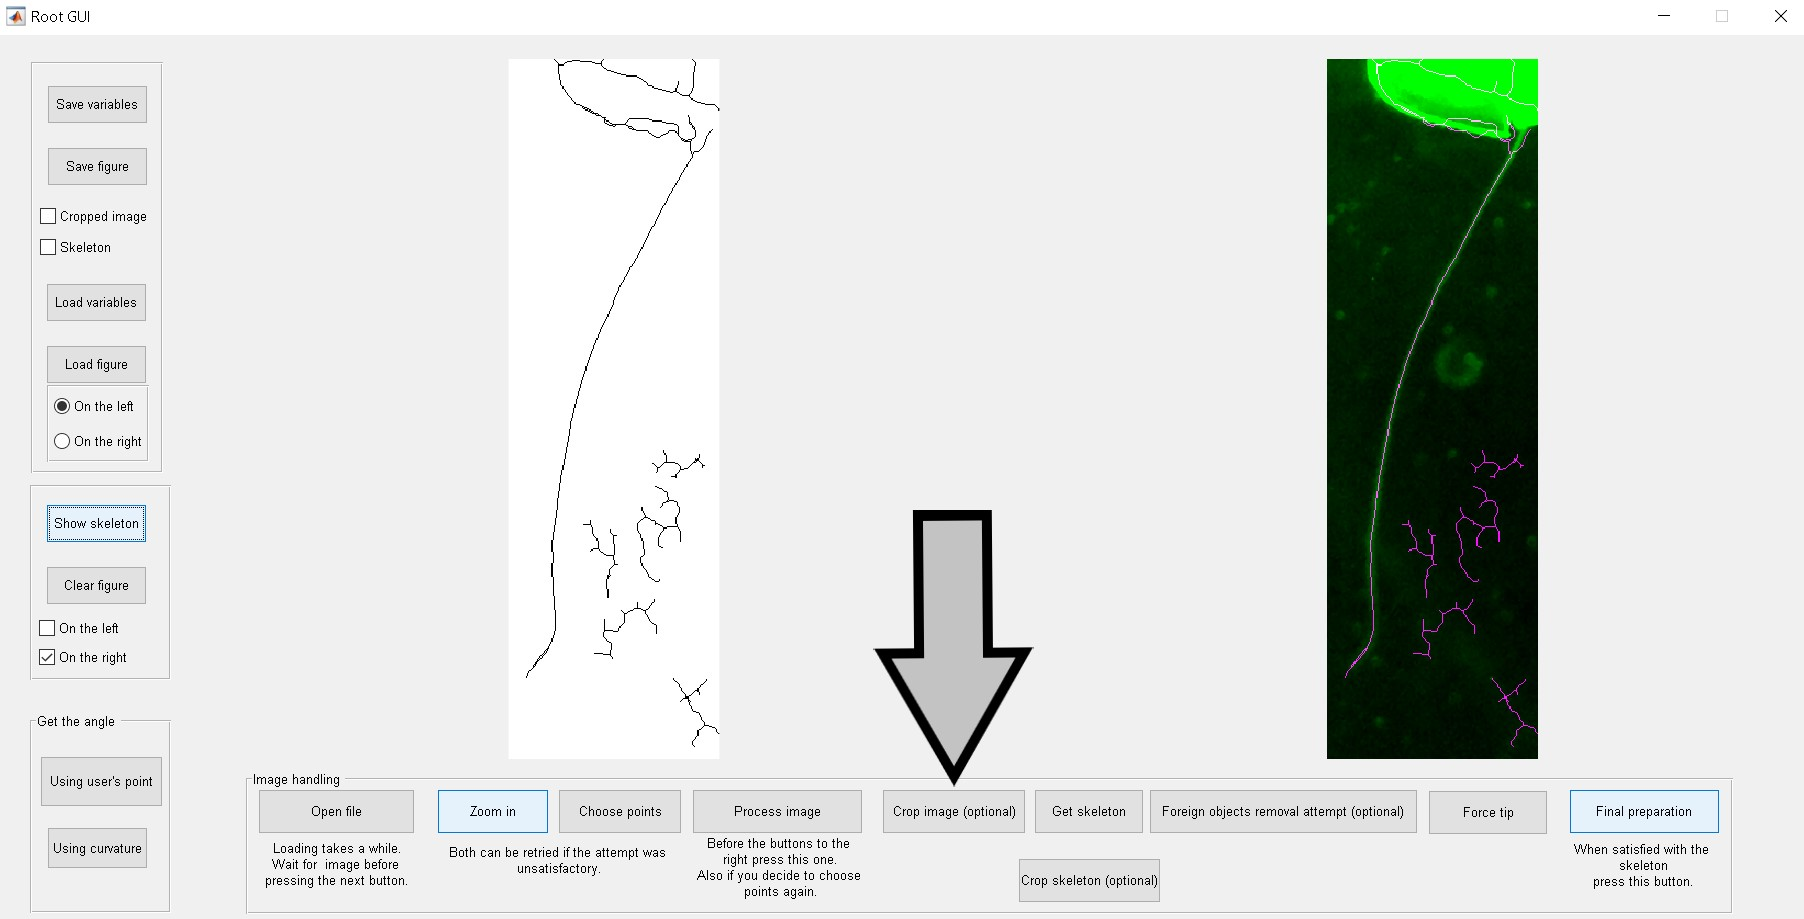
\includegraphics[width=\textwidth]{../Figures/manual/optionalC2.jpg}
	\caption{Optional step in the \textit{RootSkel} pipeline: Crop image}
	\label{fig:img47}
\end{figure}

\begin{figure}[H]
	\centering
	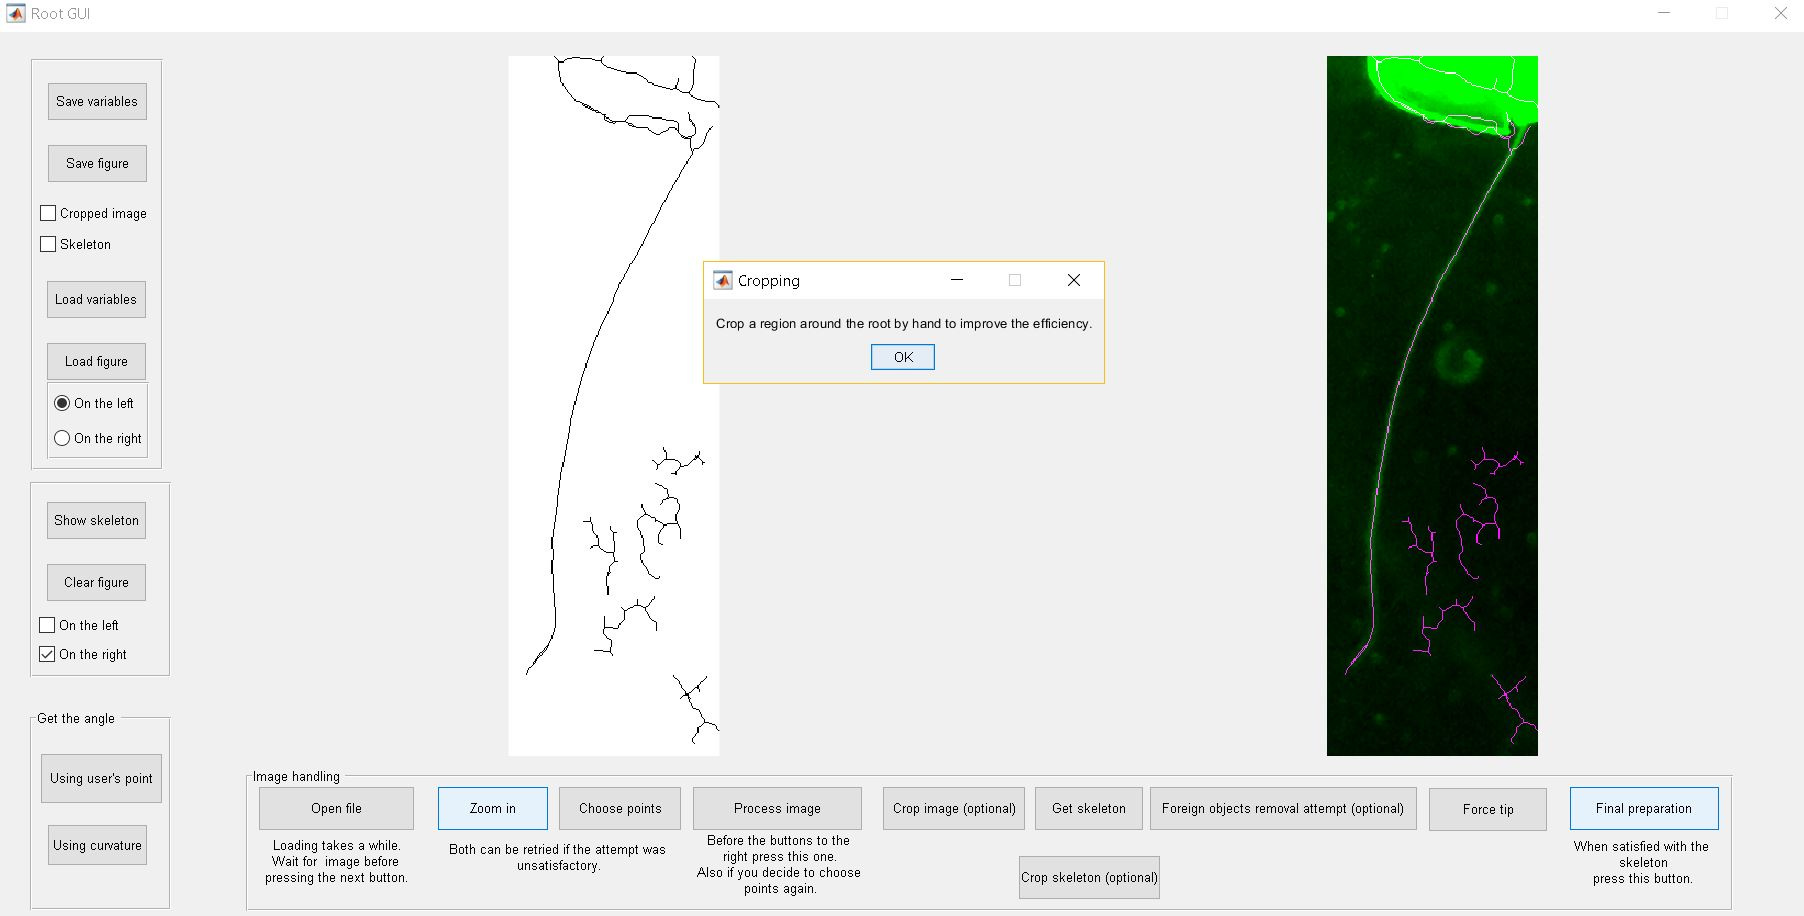
\includegraphics[width=\textwidth]{../Figures/manual/optionalC3.jpg}
	\caption{Prompt upon clicking on \textit{Crop image}}
	\label{fig:img48}
\end{figure}

\begin{figure}[H]
	\centering
	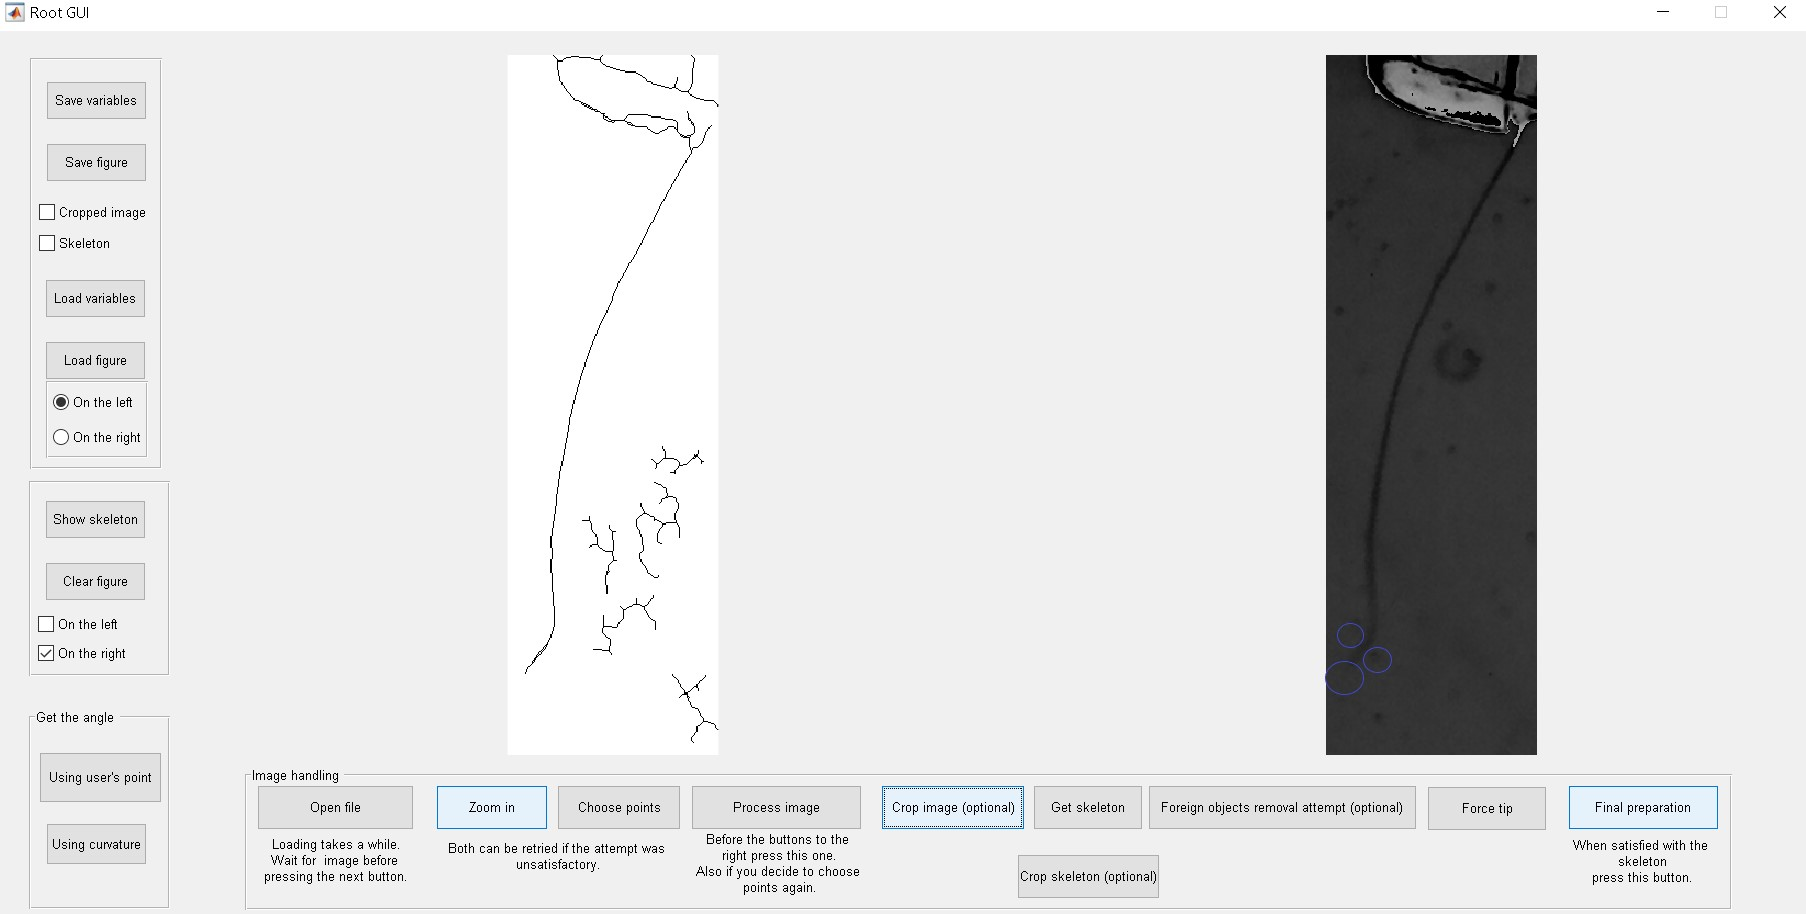
\includegraphics[width=\textwidth]{../Figures/manual/optionalC4.jpg}
	\caption{Highlighted problematic regions that need cropping}
	\label{fig:img49}
\end{figure}

\begin{figure}[H]
	\centering
	\includegraphics[width=\textwidth]{../Figures/manual/optionalC5.jpg}
	\caption{Prompt to redo the cropping}
	\label{fig:img50}
\end{figure}

\begin{figure}[H]
	\centering
	\includegraphics[width=\textwidth]{../Figures/manual/optionalC6.jpg}
	\caption{New problems in the skeleton that requires another round of cropping}
	\label{fig:img51}
\end{figure}

\begin{figure}[H]
	\centering
	\includegraphics[width=\textwidth]{../Figures/manual/optionalC7.jpg}
	\caption{Clicking on the optional step \textit{Crop image} for more cropping}
	\label{fig:img52}
\end{figure}

\begin{figure}[H]
	\centering
	\includegraphics[width=\textwidth]{../Figures/manual/optionalC8.jpg}
	\caption{Prompt to redo the cropping after the second attempt}
	\label{fig:img53}
\end{figure}

\begin{figure}[H]
	\centering
	\includegraphics[width=\textwidth]{../Figures/manual/optionalC9.jpg}
	\caption{No problems close to the root tip, only further up}
	\label{fig:img54}
\end{figure}

We still have these weird branches. But since they are not any close to the root and it seems like the skeleton near the tip is following the root, I think it's time we switch tactics.

%----------------------------------------------------------------------------------------
\subsubsection{Crop skeleton}

So now, the main problem we have is only the existence of these branches, and less the effect on the shape of the skeleton near the tip. For such problems, the \textit{Crop skeleton} step was developed. 

Let's trim some branches! Click on the \textit{Crop skeleton} button and you will see our trusty instruction pop up (see figures \ref{fig:img55} -- \ref{fig:img56}).
Now, there is no rush, we can trim the branches one by one. So first, we'll trim the left branch (see figure \ref{fig:img57}), and then we will click 'No' followed by another click on \textit{Crop skeleton}, after which we trim the second branch which leaves us with a nice and clean skeleton (see figures \ref{fig:img58} -- \ref{fig:img59}).
To see the result, we will click \textit{Final preparation} followed by \textit{Using curvature} and we see that we are getting a reasonable result (see figures \ref{fig:img60} -- \ref{fig:img61}). Success!


\begin{figure}[H]
	\centering
	\includegraphics[width=\textwidth]{../Figures/manual/optionalD1.jpg}
	\caption{Optional step in the \textit{RootSkel} pipeline: Crop skeleton}
	\label{fig:img55}
\end{figure}

\begin{figure}[H]
	\centering
	\includegraphics[width=\textwidth]{../Figures/manual/optionalD2.jpg}
	\caption{Instructions upon clicking on \textit{Crop skeleton}}
	\label{fig:img56}
\end{figure}

\begin{figure}[H]
	\centering
	\includegraphics[width=\textwidth]{../Figures/manual/optionalD3.jpg}
	\caption{Prompt to redo the cropping}
	\label{fig:img57}
\end{figure}

\begin{figure}[H]
	\centering
	\includegraphics[width=\textwidth]{../Figures/manual/optionalD4.jpg}
	\caption{A perfectly cropped root}
	\label{fig:img58}
\end{figure}

\begin{figure}[H]
	\centering
	\includegraphics[width=\textwidth]{../Figures/manual/optionalD5.jpg}
	\caption{Another nice and clean skeleton}
	\label{fig:img59}
\end{figure}

\begin{figure}[H]
	\centering
	\includegraphics[width=\textwidth]{../Figures/manual/optionalD6.jpg}
	\caption{Clicking \textit{Final preparation} and \textit{Using curvature} to compute the angle on the new skeleton}
	\label{fig:img60}
\end{figure}

\begin{figure}[H]
	\centering
	\includegraphics[width=\textwidth]{../Figures/manual/optionalD7.jpg}
	\caption{Message box displaying the computed angle}
	\label{fig:img61}
\end{figure}


%----------------------------------------------------------------------------------------
\subsubsection{Giving the problem a turning point}

For our last optional step, remember that pop up window when we click \textit{Final preparation}? The one I said we will come back to?
Well it's about time we do! So we go back to \textit{Final preparation}, only this time we will click 'Yes' when prompted (see figures \ref{fig:img62} -- \ref{fig:img63}).
Now the instructions will pop up asking us to choose the point of maximum local curvature near the tip, so we will do just that and press ENTER (see figures \ref{fig:img64} -- \ref{fig:img65}). Now a new button is enabled (see figure \ref{fig:img66}).

So we will click \textit{Using user's point} and then a message will pop up (see figure \ref{fig:img67}) with the angle and a new file will be created (see figure \ref{fig:img68}).
And that's it! We are done here! Hope you've enjoyed this friendly manual, and see you next time. 

\begin{figure}[H]
	\centering
	\includegraphics[width=\textwidth]{../Figures/manual/optionalE1.jpg}
	\caption{Last step in the \textit{RootSkel} pipeline: Final preparation}
	\label{fig:img62}
\end{figure}

\begin{figure}[H]
	\centering
	\includegraphics[width=\textwidth]{../Figures/manual/optionalE2.jpg}
	\caption{Prompt to choose the point of highest local curvature (optional)}
	\label{fig:img63}
\end{figure}

\begin{figure}[H]
	\centering
	\includegraphics[width=\textwidth]{../Figures/manual/optionalE3.jpg}
	\caption{Instructions to choose the point of highest local curvature}
	\label{fig:img64}
\end{figure}

\begin{figure}[H]
	\centering
	\includegraphics[width=\textwidth]{../Figures/manual/optionalE4.jpg}
	\caption{Choosing the point of highest local curvature}
	\label{fig:img65}
\end{figure}

\begin{figure}[H]
	\centering
	\includegraphics[width=\textwidth]{../Figures/manual/optionalE5.jpg}
	\caption{Clicking on \textit{Using users input} upon clicking on the point of highest local curvature}
	\label{fig:img66}
\end{figure}

\begin{figure}[H]
	\centering
	\includegraphics[width=\textwidth]{../Figures/manual/optionalE6.jpg}
	\caption{Message box displaying the computed angle}
	\label{fig:img67}
\end{figure}

\begin{figure}[H]
	\centering
	\includegraphics[width=0.6\textwidth]{../Figures/manual/optionalE7.jpg}
	\caption{The created .csv files with the computed angles showing up on the LHS of the MATLAB GUI}
	\label{fig:img68}
\end{figure}


%----------------------------------------------------------------------------------------
%----------------------------------------------------------------------------------------
%----------------------------------------------------------------------------------------
\chapter{On the data set}

The data set used can be found on \url{https://imperialcollegelondon.app.box.com/folder/50485327378}.

%----------------------------------------------------------------------------------------
%----------------------------------------------------------------------------------------
\section{Challenging images}\label{subsec:challengingImages}

%There is a very low contrast between the background and the roots, so that one could hardly recognise the roots on some images [INSERT EXAMPLE IMAGE HERE].
As mentioned in the report, the data set we were working on contained highly challenging images (see figure \ref{fig:challenginRoots}), this was due to
\begin{itemize}
	\item Low contrast between roots and background; the roots were almost not discernible for the human eye without previous treatment of the image (see subfigure \ref{figsub:lowContrast})
	\item Lots of noise or objects that we classified as noise as there was no apparent structure to it (see subfigure \ref{figsub:noisy})
	\item Different noise patterns, i.e. inconsistency, across the images; the noise was subtle or hiding and could only made visible on filtered images (see subfigure \ref{figsub:noisy})
	\item Numerous objects that were of no interest, especially the ones interfering with our object of interest (see subfigure \ref{figsub:stickyObject})
	\item Low resolution of the images or object of interest itself taking up only a small fraction of the whole image. 
\end{itemize}
Highly pixeled images made not only the preprocessing but especially the curvature computing part challenging; also various MATLAB functions do not work well on sparse data.
In section \ref{futuredataAquis} we make suggestions for future data collection.

\begin{figure}[H] 
	\begin{subfigure}[b]{0.5\linewidth}
		\centering
		\includegraphics[width=0.75\linewidth]{2018-03-08_1000.jpg} 
		\caption{Changing light reflection (root on the LHS\\ is lost), low contrast} 
		\label{figsub:reflection} 
		\vspace{4ex}
	\end{subfigure}%% 
	\begin{subfigure}[b]{0.5\linewidth}
		\centering
		\includegraphics[width=0.75\linewidth]{2018-02-28_2030.jpg} 
		\caption{Foreign object sticking to root, \\blurry regions, other objects} 
		\label{figsub:stickyObject} 
		\vspace{4ex}
	\end{subfigure} 
	\begin{subfigure}[b]{0.5\linewidth}
		\centering
		\includegraphics[width=0.75\linewidth]{2018-04-24_1840.jpg} 
		\caption{Noisy image, many objects of same colour} 
		\label{figsub:noisy} 
	\end{subfigure}%%
	\begin{subfigure}[b]{0.5\linewidth}
		\centering
		\includegraphics[width=0.75\linewidth]{2018-03-06_2000.jpg} 
		\caption{Low contrast, roots touching each other} 
		\label{figsub:lowContrast} 
	\end{subfigure} 
	\caption{Problems of images; images taken from our data set: (A) 2018-03-08\_1000.jpg, (B) 2018-02-28\_2030.jpg, (C) 2018-04-24\_1840.jpg, (D) 2018-03-06\_2000.jpg}
	\label{fig:challenginRoots} 
\end{figure}


%----------------------------------------------------------------------------------------
%----------------------------------------------------------------------------------------
\section{Suggestions for future data acquisition}\label{futuredataAquis}

We will give some suggestions on how to improve the quality of the images in the future. More advice on things that should be considered when capturing the images can be found in PlantCV \cite{plantCV}. It should be emphasised that it is always best to try to reduce potential image processing problems up front, instead of trying to work on bad and inconsistent images \cite{plantCV}. With this goal in mind, it might be useful to capture a test image beforehand and process it using PlantCV \cite{plantCV} or any other similar software before acquiring a full data set \cite{plantCV}.   

In the following we will point out some common pitfalls that should be avoided in the future in order for \textit{RootSkel} to produce more accurate and robust results.


%----------------------------------------------------------------------------------------
\subsection{Consistent images}

In general, one should ensure to keep the conditions over one experiment stable as far as possible. We understand that this is far harder to achieve in a dynamic system as the one to capture electrotropism compared to a gravitropism setup; the latter usually being done in a stabilising agar gel. 
This includes a constant number of tubes and roots, constant water level or surface and no external movement to the roots or the tubes to keep the noise distribution as constant as possible. One should make sure that the camera is set at exactly the same vantage point in each image, if necessary, by using a size marker \cite{plantCV}. 
Roots that are affected by change in reflections or lightning (e.g. by people walking into the growth room) have been proven to be very hard to handle and are often lost in the preprocessing step. If lightning is changing one might want to use a colour card or a white balance card to "normalise" the lightning across images \cite{plantCV}. 
Keeping the medium clean of dirt and bubbles as far as possible is likely to make the preprocessing step easier and faster as well.
%also improve the preprocessing step. 


%----------------------------------------------------------------------------------------
\subsection{Increase of the contrast}

In the current image data set there is not enough contrast between the target object (the root) and the background. This makes it difficult to distinguish the two of them, even by eye. It is advisable to work towards achieving a good level of contrast between the roots and the background, e.g. by adding black background behind the roots or materials like blue material \cite{plantCV}. 
%It is advisable to work towards achieving a higher contrast in the images, so roots can be clearly distinguished from the background, also by eye.


%----------------------------------------------------------------------------------------
\subsection{No objects interfering with the object of interest}

The experimentalist should make sure to avoid crossovers, i.e. that there are no objects interfering with the object of interest. This could be a neighbouring root (see subfigure \ref{figsub:lowContrast}) or any other similar looking objects (see subfigure \ref{figsub:stickyObject}) that are difficult to discern even by eye, throughout the experiment or at least as long as we want to analyse this root's angle. 

%llumination different — challenge to get background right
%local thresholds maybe?


%%----------------------------------------------------------------------------------------
%\subsection{More focus on images}


%----------------------------------------------------------------------------------------
\subsection{Higher resolution}

As the highly pixeled nature of the images did cause problems also in the angle computation, it is recommendable to try to increase the resolution of the images (e.g. to 10 Mexapixels, in the current images we use 5-8 Megapixels, that is dimensions between 3280\(\times\)2464 and 2592\(\times\)1944). One could also try to zoom into the roots or even one single root so our actual object(s) of interest take up a bigger fraction in the images instead of spending resolution on things that are of no interest. 

Applying a non-reversible compression, such as converting the images to JPEG file format can be unsuitable for data processing \cite{french2009high} as it creates coarser images and removes details in regions that we as humans perceive least well \cite{french2009high}. It usually significantly affects spatial resolution of colour \cite{french2009high}. In any case, JPEG images should always be saved with the highest quality settings to prevent the quality to be reduced too much. 
%
%A risk might be the lossy (i.e. non-reversible) compression step to JPG file format after taking the photos which creates coarser images and details to be removed.
%that might cause or contribute to the low resolution of the images. 
One could attempt to use other formats to save the images, including lossless formats such as PNG or TIFF file format.

As a last suggestion, different cameras could be compared to see if it does have an effect on the quality of the images. 

%Better camera, less waste of resolution
%improve spatial resolution, other format? no compression?


%----------------------------------------------------------------------------------------
%----------------------------------------------------------------------------------------
%----------------------------------------------------------------------------------------
\chapter{Literature review}\label{litreview}

The following 6 pages gives an overview of different software image processing tools for plants from the last 10 years. All have their strengths and weaknesses; popular ones are highlighted by a read margin. An overview of tools developed before the tool \textit{RootTrace} can be found in \cite{french2009high}.

%\begin{figure}[H]
%	\centering
%	\includegraphics[width=\textwidth]{../Figures/literature_final.pdf}
%	\caption{Software image processing tools for plants in the last 10 years: All have their strengths and weaknesses; popular ones are highlighted by a read margin. An overview of tools developed before \textit{RootTrace} can be found in \cite{french2009high}.}
%	\label{fig:lit}
%\end{figure}

\includepdf[pages=-, angle=90]{../Figures/literature_final.pdf}


There are a number of web-based software tools to visualise and analyse root system architecture available; the ones that are still being supported include:
\begin{itemize}
	\item \textit{ObjectJ} [\url{http://www.plant-image-analysis.org/software/objectj}]
	\item \textit{Rhizo-II Root Biometrics Suite} \url{[https://www.psrg.org.uk/plant-biometrics.html]}
	\item \textit{Rootfly} [\url{http://www.plant-image-analysis.org/software/rootfly}].
\end{itemize}

In recent years, a number of Machine Learning and Deep Learning plant tools have been developed \cite{pound2017deep,lee2018automated,navarro2016machine}; however, they often require substantial hardware systems including a GPU (Grahics Processing Unit) to train the complex networks in a feasible time.
